\documentclass{article}
%
\newtheorem{theorem}{Theorem}
\newtheorem{definition}{Definition}
\newtheorem{proof}{Proof}
\renewcommand{\thetheorem}{\arabic{section}.\arabic{theorem}}
\renewcommand{\thedefinition}{\arabic{section}.\arabic{definition}}
\renewcommand{\theproof}{\arabic{section}.\arabic{proof}}

%
\usepackage[utf8]{inputenc}
\usepackage{amsmath}
\usepackage{amssymb}
\usepackage{graphicx}
\usepackage{amsfonts}
\usepackage{ mathrsfs }
%
\DeclareMathOperator\erf{erf}
%
\textwidth = 6.1in
\oddsidemargin=0.2in %add 1in for left margin
\evensidemargin=0.2in %add 1in for right margin

\topmargin=-.3in
\textheight=8.5in


%\title{Module Course: ODEs, PDEs, and Linear Algebra}
%\author{\\ Nicholas A. Battista}
%\date{Modified: July 31, 2015 \\
%Created: June 3, 2015}



\begin{document}

%\maketitle
\begin{center}
$ $\\
\vspace{0.5in}
\huge Module Course: ODEs, PDEs, and Linear Algebra
\end{center}
$ $\\
\vspace{0.25in}
%
\pagestyle{plain}
\setcounter{page}{1}
\pagenumbering{Roman}
%
% COVER PICTURE
\begin{figure}[hb] 
\centering 

\includegraphics[width=5.5in]{cover.png} 
\caption[Close up of \textit{Hemidactylus} sp.] {\emph{Numerical Microscopy: The Trabeculated Ventricle of an 84hpf  Zebrafish Embryonic Heart} Mathematical model and simulation of an embryonic zebrafish heart at 84 hours post fertilization. Blood cells can be seen flowing into the ventricle during the diastole phase. Blood flow plays a critical role in heart development, as hemodynamic forces act as signaling mechanisms to regulate a wide host of developmental processes at the cellular and genetic level.} 
\end{figure}
%
$ $\\
\vspace{0.25in}
%
\setcounter{page}{1}
\pagenumbering{arabic}
%
\begin{center}
\Large Nicholas A. Battista\\
\Large Modified: August 14, 2015\\
\Large Created: June 3, 2015\\
\end{center}

\newpage
\graphicspath{{./Intro/}}

\section{Introduction}

Welcome! In this short 5 day course, we will cover a variety of topics pertaining to analytical methods in applied mathematics. Most of these topics have been chosen in part because this material that seems to have a way of falling through the cracks of most undergraduate curriculums in mathematics and because they are traditionally not covered during the first year sequence in methods of applied mathematics. 

The tentative list of topics we will cover is below: 
\begin{enumerate}
%
\item A review of undergraduate ODEs
\begin{itemize}
\item Separable Equations
\item First-Order: Integrating Factor
\item Homogeneous vs. Nonhomogeneous Equations
\item Solving for Complementary Solutions
\begin{itemize}
\item Linear constant coefficient ODEs
\end{itemize}
\item Solving for Particular Solution:
\begin{itemize}
\item Undetermined Coefficients
\item Variation of Parameters
\end{itemize}
\item Bonus Methods:
\begin{itemize}
\item Transform Methods (i.e., ``Euler" type, Ricatti type, etc)
\item Laplace Transforms
\item Non-dimensionalization
\item Introduction to Dynamical Systems, e.g., systems of ODEs
\end{itemize}
\end{itemize} 
%
\item General Sturm-Liouville Theory
\begin{itemize}
\item Orthogonal Functions
\item Fourier Series
\item Orthogonal Polynomials as a Complete Basis
\end{itemize}
%
\item Greens Functions
%
\item Linear PDEs
\begin{itemize}
\item Classification of PDEs
\item Derivations of classical linear PDEs
\item Method of Characteristics
\item Separation of Variables
\item Fourier Transforms / Laplace Transforms
\item Similarity Solutions
\item Method of Images
\end{itemize}
%
\item Physics!
\begin{itemize}
\item Newton's Laws of Motion
\item Conservation Laws
\item Lagrangian Formulation of Mechanics
\item Hamiltonian Formulation of Mechanics
\end{itemize}
%
\item Big Picture Numerical Linear Algebra
\begin{itemize}
\item Linear systems, the bread and butter.
\item Nonlinear systems, root-finding, and iterative methods - oh my!
\item Eigen-fun: a story of eigenvalues, eigenvectors, and love.
\end{itemize}
%
\end{enumerate}

Please note that these notes may not be complete at this time. Please check back periodically as more sections will be added...\emph{when my code is compiling.} 
\newpage
\graphicspath{{./Undergrad_ODEs/}}

\section{Review of Undergrad. ODEs}

Undergraduate Ordinary Differential Equations, or Calculus 4, is mostly a blitz of various analytical methods for solving initial value problems for linear (and some special case non-linear) differential equations. 

In this section we will review the following methods:

\begin{enumerate}
\item Separable Equations
\item First-Order: Integrating Factor
\item Homogeneous vs. Nonhomogeneous Equations
\item Solving for Complementary Solutions
\begin{itemize}
\item Linear constant coefficient ODEs
\end{itemize}
\item Solving for Particular Solution:
\begin{itemize}
\item Undetermined Coefficients
\item Variation of Parameters
\end{itemize}
\item Bonus Methods and Conceptual Fun:
\begin{itemize}
\item Transform Methods (i.e., ``Euler" type, Ricatti type, etc)
\item Laplace Transforms
\item Non-Dimensionalization
\item Introduction to Dynamical Systems, e.g., systems of ODEs
\begin{itemize}
\item Eigenvalues and Systems of Linear Homogeneous ODE
\item The Matrix Exponential
\item Non-homogeneous Linear Systems
\item Non-linear Systems of ODEs
\end{itemize}
\end{itemize}
\end{enumerate}

Since undergraduate ODEs does not have much theory, we will try to motivate each method, when possible, otherwise sit back and enjoy the following stampede of methods!


%%%%%%%%%%%%%%%%%%%%%%%%%%%%%%%%
%
% SEPARABLE EQUATIONS
%
%%%%%%%%%%%%%%%%%%%%%%%%%%%%%%%%

\subsection{Separable Equations}

Perhaps the most natural method to solve ODEs comes from ideas of calculus, where we simply want to integrate anything and everything possible. The differential equations we are able to solve via pure integration are of the form, where you can \emph{separate} the dependent variable and indepedent variables entirely, i.e., if we have the following ODE to solve,
$$\frac{dy}{dx} = f(x,y) = g(x) h(y),$$ with $y(a) = y_a$ as initial data. 

We can then separate the equation, 

$$\frac{dy}{h(y)} = g(x) dx.$$

Now integrating  both sides we can get a functional relationship between $y$ and $x$. Unfortunately, sometimes this relationship is nonlinear or transcendental, making it difficult to write a solution like $y=y(x)$; however, we can still use the initial data to solve for the integration constant. 

For example consider, $$\frac{dy}{dt} = -y(1-y),$$ with $y(0)=2$. We can then go through the separation method to find,

\begin{align*}
\frac{dy}{y(1-y)} &= -dt \\
\int \frac{1}{y(1-y)} dy &= \int -dt \\
\log(y) - \log(1-y) &= -t + C \\
\frac{y}{1-y} =&= Ae^{-t} 
\end{align*}

and hence doing a little algebra we find that $$y(t) = \frac{Ae^{-t}}{1+Ae^{-t}}.$$

Now using the initial value information we can get $A$, 

$$y(0)=2 \Rightarrow 2 = \frac{A}{1+A} \Rightarrow A = -2.$$

Therefore our solution is $y(t) = \frac{-2e^{-t}}{1-2e^{-t}}.$ Note that this solution will blow up for finite time, namely when $e^{-t} = \frac{1}{2}$ or $t=\ln\left(\frac{1}{2}\right)$.




%%%%%%%%%%%%%%%%%%%%%%%%%%%%%%%%
%
% First-Order Integrating Factor
%
%%%%%%%%%%%%%%%%%%%%%%%%%%%%%%%%

\subsection{First-Order Integrating Factor}

The world would be very nice, but boring, if all first-order differential equations were separable. Note: Not all separable equations are useless $\rightarrow$ some describe many processes in population biology or black hole thermodynamics! \\

To simply make an equation not separable, we just need to tack on one extra term; however, we will restrict ourselves to linear first-order equations now of the form,

\begin{equation}
\label{1st_order_ode} \frac{dy}{dx} + p(x) y(x) = q(x),
\end{equation}

where we assume $p(x)$ and $q(x)$ are continuous. To solve the above equation we consider the left hand side of (\ref{1st_order_ode}) to be the result of a product rule. However, to make it such we need to multiply all the terms by fudge factor given in exponential form, also known as the \emph{integrating factor},

$$e^{\mu(x)}  = e^{\int p(x) dx},$$

thereby giving $\frac{d}{dx} e^{\mu(x)} = p(x) e^{\mu(x)}$ since $\frac{dv}{dx} = p(x).$ Doing so we see the product rule gives, 

$$\frac{d}{dx} \left[ e^{\int p(x) dx } y(x) \right] = e^{\int p(x) dx} \left[ \frac{dy}{dx} + p(x) y(x) \right] = e^{\int p(x) dx} q(x).$$

Hence to solve (\ref{1st_order_ode}), we need to integrate both sides and then easily solve for $y(x)$, e.g.,

\begin{align*}
\frac{d}{dx} \left[ e^{\int p(x) dx } y(x) \right] &= e^{\int p(x) dx} q(x) \\
\int \frac{d}{dx} \left[ e^{\int p(x) dx } y(x) \right] dx &= \int e^{\int p(x) dx} q(x) dx \\
e^{\mu(x) } y(x) &= \int e^{\mu(x) } q(x) dx
\end{align*}

and therefore we find that $$y(x) = e^{-\mu(x)}  \int e^{\mu(x)} q(x) .$$

\subsubsection{Example: Integrating Factor}

Let's do an example! Consider $$\frac{dy}{dt} +  \frac{1}{3} t^2 y(t) = t^2.$$

Using the integrating factor approach we first identity $e^{\mu(t)}$ as $$e^{\mu(t)} = e^{\int \frac{1}{3} t^2 dt } = e^{t^3}.$$

Then using the methodology developed above, we see $$y(t) = e^{-t^3} \int  e^{t^3} t^2 dt,$$

and hence $$y(t) = \frac{1}{3} + C e^{-t^3},$$ 

where $C$ can be solved using initial data.



%%%%%%%%%%%%%%%%%%%%%%%%%%%%%%%%
%
% Honogeneous vs. Non-homogeneous Equations
%
%%%%%%%%%%%%%%%%%%%%%%%%%%%%%%%%

\subsection{Homogeneous vs. Non-homogeneous Equations}

Before we begin our trajectory into higher order linear differential equations, we are going to set a clear discrepancy between homogeneous and non-homogeneous equations. In two words, a homogeneous equation is when we have a bunch of dependent variable stuff equal to zero, i.e., 

$$\hat{L}y(x) =  c_n(x) \frac{d^n y}{dx^n} + c_{n-1}(x) \frac{d^{n-1} y}{dx^{n-1}} + \ldots + c_2(x) \frac{d^2 y}{dx^2} + c_1(x) \frac{dy}{dx} + c_0(x) y = 0.$$

On the other hand a non-homogeneous equation looks like the above, except with non-zero right hand side, e.g., 

$$\hat{L}y(x) = c_n(x) \frac{d^n y}{dx^n} + c_{n-1}(x) \frac{d^{n-1} y}{dx^{n-1}} + \ldots + c_2(x) \frac{d^2 y}{dx^2} + c_1(x) \frac{dy}{dx} + c_0(x) y = q(x).$$

The reason we make clear the distinction is because if we consider a solution to the \emph{non-homogeneous} problem, call it $y_P(x)$, we have 

$$\hat{L} y_P(x) = q(x),$$ while a solution for the homogenous problem, call it $y_C(x)$, looks like $$\hat{L} y_C(x) = 0.$$

Therefore if we consider a combined solution, $$y(x) = y_C(x) + y_P(x),$$ we have

$$\hat{L} y(x) = \hat{L} y_C(x) + \hat{L} y_P(x)  = q(x).$$

Hence if we are trying to solve a non-homogeneous problem, we see it is \emph{necessary} to solve the homogeneous problem as well. We call the solution to the homogeneous problem the \emph{complementary} solution, while the solution to the non-homogeneous problem is called the \emph{particular} solution. \\

Furthermore we note that any scaling multiple of the complementary solution is also a problem to the homogeneous problem, i.e., $$\hat{L}[ \alpha y_C(x) ] = 0,$$

where $\alpha\in\mathbb{C}.$




%%%%%%%%%%%%%%%%%%%%%%%%%%%%%%%%
%
% Linear Constant Coefficient ODEs (2nd Order)
%
%%%%%%%%%%%%%%%%%%%%%%%%%%%%%%%%

\subsection{Linear Constant Coefficient ODEs}

We will discuss equations of the form, 

$$\hat{L}y(x) =  c_n \frac{d^n y}{dx^n} + c_{n-1} \frac{d^{n-1} y}{dx^{n-1}} + \ldots + c_2 \frac{d^2 y}{dx^2} + c_1 \frac{dy}{dx} + c_0y = 0,$$

where $\{ c_j \}_{j=0}^{n} \in \mathbb{R}.$ For equations of this form we will show that our solution technique assumes an ansatz for a solution and by doing so terms this differential problem into more an algebraic polynomial root-finding issue. We also note that since this is an $n^{th}$ order homogeneous equation, we need to find $n$ linearly independent solutions for our complementary solution.

To illuminate this idea better further, we will show the possibilities for second-order linear constant coefficient ODEs. 

We now consider the following ODE,
\begin{equation}
\label{2nd_order_cc_ode} a \frac{d^2 y}{dx^2} + b \frac{dy}{dx} + c y = 0,
\end{equation}

with initial data of the form $y(0) = y0$ and $y'(0) = y_0^P.$ We assume solutions of the following form $$y = e^{rt},$$ where $r\in\mathbb{C}$. Continuing with this path we see

\begin{align*}
a \frac{d^2 y}{dx^2} + b \frac{dy}{dx} + c y &= a \frac{d^2}{dx^2}\left[e^{rt}\right] + b \frac{d}{dx}\left[e^{rt}\right] + c \left[e^{rt}\right]\\
& = a r^2 e^{rt} + b r e^{rt} + c e^{rt} \\
& = e^{rt} \Big[ a r^2 + b r + c \Big] = 0
\end{align*}

and hence we now need to solve $$a r^2 + b r + c = 0,$$ and then will have the numeric values or $r$ to build our complementary solution. We call this polynomial the \emph{characteristic equation}. 

Moreover we note at this junction that we need $n$ linearly independent solutions for our complementary solution, and in the above we had a second-order linear ODE and obtained a second-order polynomial to find the roots of. In this second-order example, we will have three possible cases that the roots can fall into. Naturally this goes back to properties of quadratic equations and when there are real, complex, or double roots. 

We will highlight each case with an example. 

\begin{itemize}

%
% CASE 1
%
\item[Case 1]: $b^2 - 4ac > 0$ (real roots)

Consider the following example $$y'' -  y' - 2y = 0.$$

Substituting our ansatz, $y= e^{rt}$ we find we get the following algebraic equation to solve $$r^2 - r - 2=0.$$

Solving this equation we find that $r = \{ -1,2\}$ and hence we get two linearly independent solutions that solve the homogeneous problem above, $$\{ e^{-x}, e^{2x}\},$$

and so our complementary solution is $$y_C(x) = \alpha_1 e^{-x} + \alpha_2 e^{2x}.$$

%
% CASE 2
%
\item[Case 2]: $b^2 - 4ac < 0$ (complex roots)

Consider the following example $$y''+2y' + 2y = 0.$$

Again, substituting our ansatz, $y=e^{rt}$, we get the following characteristic equation $$r^2+2r+2=0.$$

Solving this equation we find $r = \{ 1-i,1+i\}$ and so our linearly independent solutions are $\{ e^{(1-i)x}, e^{(1+i)x}\}$. We can easily write the complementary solution as $$y_C(x) = \alpha_1 e^{(1-i)x} + \alpha_2 e^{(1+i)x},$$

but we will massage our solutions to a more friendly form! After much algebra, we find we can write the above as:

$$y_C(x) = e^{x} \Big[ \alpha_1 \cos(x) + \alpha_2 \sin(x) \Big.$$

In general if we find our complex roots to be $\{ a-bi, a+bi \},$ we can write our complementary solution as

$$y_C(x) = e^{ax} \Big[ \alpha_1 \cos(bx) + \alpha_2 \sin(bx) \Big].$$


%
% CASE 3
%
\item[Case 3]: $b^2-4ac = 0$ (root with multiplicity $> 1$.)

Consider the following example $$y'' - 6y' + 9y = 0.$$

Using our ansatz, $y=e^{rt}$, we obtain the following characteristic equation $$(r-3)^2 = 0.$$

Hence solving this equation we find that $r=3$ is a double root, i.e., a root with multiplicity $> 1$. Therefore if we tried to write our complementary solution is a similar way to \emph{Case 1}, we would have $$y_C(x) = \alpha_1 e^{3x} + \alpha_2 e^{3x} = \alpha ^{3x},$$

and thereby only have \emph{ONE} linearly independent solution, when we need two! The method we will employ to find this second solution is a special (easy) case of \emph{Reduction of Order}. We assume the second linearly independent solution $y_2(x)$ has the form $$y_2(x) = v(x)y_1(x) = v(x) e^{3x},$$ where $y_1(x) = e^{3x}$ is the linearly independent solution we do have!

Plugging this into the ODE we get,
\begin{align*}
y_2'' - 6y_2' + 9y_2 &= [v'' y_1 + 2v'y' + vy_1''] - 6[v'y_1 + vy_1'] + 9vy_1 \\
&= [v''y_1 +2v'y_1' - 6v'y_1] + v(x) [ y_1'' - 6y_1' + 9y_1] \\
&= v''e^{3x} + (3)2v'e^{3x} - 6v'e^{3x} \\
&= e^{3x} \Big[ v'' \Big] = 0 \\
\end{align*}

and therefore we need to solve $v'' = 0$ and find $v(x) = \beta x + \gamma.$ Hence our second linearly independent solution is $$y_2(x) = ( \beta x+\gamma)e^{3x},$$

and our complementary solution is

$$y_C(x) = \alpha e^{3x} + ( \beta x+\gamma)e^{3x} = ( \tilde{\alpha} + \beta x )e^{3x},$$

where $\tilde{\alpha} = \alpha+\gamma$, but is just another constant to be found using the initial data afterall, so it's nothing too fancy!

\end{itemize}



%%%%%%%%%%%%%%%%%%%%%%%%%%%%%%%%
%
% Solving for the particular solutions!
%
%%%%%%%%%%%%%%%%%%%%%%%%%%%%%%%%

\subsubsection{Solving for the Particular Solution}

In this section we are concerned with finding the particular solution, $y_P(x)$, for non-homogeneous equations. We will assume that we already found the complementary solution, i.e., the solution to the homogeneous equation, $y_C(x)$. We are concerned with the particular solutions of linear constant-coefficient equations, i.e., 

\begin{equation}
\label{nonhomogeneous_eq} c_n(x) \frac{d^n y}{dx^n} + c_{n-1}(x) \frac{d^{n-1} y}{dx^{n-1}} + \ldots + c_2(x) \frac{d^2 y}{dx^2} + c_1(x) \frac{dy}{dx} + c_0(x) y = q(x).
\end{equation}

Like in the previous section, we illustrate this concept with $2^{nd}$ order linear constant coefficient equations, $$c_2 y'' + c_1 y' + c_0 y = q(x).$$

We will describe two methods for finding the \emph{particular} solution,
\begin{enumerate}
\item Undetermined Coefficients
\item Variation of Parameters
\end{enumerate}

\begin{itemize}
%
% Undetermined Coefficients
%
\item {\bf{Undetermined Coefficients:}}

This method of finding a particular solution is similar to that of ``guess and check!". This method will only work for special cases of $q(x)$, namely if $q(x)$ belongs to the following families of functions $\{ a_n x^n +\ldots a_1 x+a_0, e^{ax}, \sin(ax),\cos(ax)\}$, or any products of those. 

\begin{itemize}
\item \emph{Example 1:} Consider the following example, $$y'' - y' - 2y = 6x^2.$$

Recall we found the complementary solution to be $y_C(x) = \alpha_1 e^{-x} + \alpha_2 e^{2x}.$ Now since $q(x)$ is a polynomial, we will assume a polynomial form for $y_P(x)$, i.e., we will let $y_P(x) = c_1 x^2 + c_2 x + c_3.$

Substituting our particular solution into the ODE gives
\begin{align*}
y''-y'-2y= 6x^2 &= \frac{d^2}{dx^2}(c_1 x^2 + c_2 x + c_3) - \frac{d}{dx} ( c_1 x^2 + c_2 x + c_3) - 2(c_1 x^2 + c_2 x + c_3) \\
&= (2c_1) - (2 c_1 x + c_2) - 2(c_1 x^2 + c_2 x + c_3) \\
&= [-2 c_1] x^2 - 2[ c_1 + c_2 ]x + [2c_1 - c_2 -2c_3] 
\end{align*}

Hence we see that we have the following system of equations to solve
\begin{align*}
-2 c_1 &= 6 \\
-2c_1 - 2 c_2 &= 0 \\
2c_1 - c_2 - 2c_3 &= 0\\
\end{align*}

Solving this system we find that $c_1 = -3$, $c_2 = 3$, and $c_3 = -\frac{9}{2}.$ Thereby making our particular solution $y_P(x) = -3x^2+3x-\frac{9}{2}.$ Hence our full solution to this non-homogeneous equation is
$$y(x) = y_C(x) + y_P(x) =  \alpha_1 e^{-x} + \alpha_2 e^{2x} + \Big[-3x^2+3x-\frac{9}{2}\Big],$$

up to using the initial data to solve for $\{\alpha_1,\alpha_2\}.$ \emph{Note} that even though $q(x)$ did not have a linear term of constant term, the particular solution did have those components. Hence we have to make sure to include all the polynomial terms at the same order and below as $q(x)$.
\end{itemize}

We can do a similar process if $q(x)$ takes on the other functional forms. Below is a table for what particular solution to ``guess" for each $q(x)$.

$$\begin{array}{|c|c|}
\hline 
{\bf{q(x)}}   & {\bf{y_P(x)}} \\
\hline
e^{ax}   & c_1 e^{ax}\\
\hline
\sin(bx) & c_1 \sin(bx) + c_2\cos(bx) \\
\hline
\cos(bx) & c_1 \sin(bx) + c_2\cos(bx) \\
\hline
\beta \sin(bx)+ \gamma \cos(bx) & \sin(bx) + c_2\cos(bx) \\
\hline
a_n x^n \ldots a_2x^2 + a_1 x + a_0 & c_n x^n \ldots c_2x^2 + c_1 x + c_0 \\
\hline
\end{array}$$

\begin{itemize}
\item \emph{Example:} Resonance

One other subtle point to make is in the case when $q(x) = e^{ax}$. If our complementary solutions are exponential functions, it is possible that our complementary solutions may already include a term of $e^{ax}$, i.e., $y_C(x) = \alpha_1 e^{ax} + \alpha_2 e^{bx}.$ In this case, we will have \emph{resonant} solutions. 

Our particular solution will then take on a term like $y_P(x) = c_1 x e^{ax},$ analogous to what we did in the case of multiple roots using Reduction of Order.

\end{itemize}


%
% Variation of Parameters
%
\item {\bf{Variation of Parameters:}}

The next method for finding particular solutions assumes we already know what the complementary solutions are. Like the last case, we will assume we are trying to solve a $2^{nd}$ order linear ODE. \emph{Note} this method does not only work for linear constant coefficient ODEs, unlike undetermined coefficients.  This method will work for higher order equations analogously (the algebra just gets a \emph{bit} more undesirable).

Called, \emph{variation of parameters}, it is a method that exploits a more general \emph{reduction of order} technique. We begin with the set of fundamental solutions $\{ y_1(x), y_2(x) \}$, i.e., where $y_C(x) = \alpha_1 y_1(x) + \alpha_2 y_2(x).$ We now assume the particular solution takes a reduction-of-order-form,
\begin{equation}
\label{vop_form} y_P(x) = u_1(x) y_1(x) + u_2(x) y_2(x),
\end{equation}

where $\{ u_1(x), u_2(x) \}$ are unknown functions that we now set out to find! To motivate this concept, we will try to find the particular solution to $$y''+ p(x)y' + r(x) y = q(x),$$ with already found fundamental solutions $y_1(x)$ and $y_2(x)$.

We begin with the following constraint $$u_1' y_1 + u_2' y_2 = 0.$$ The reasons for this choice on constraint are not immediately obvious, but upon doing so we see that the above constraint makes the derivative of $y_P(x)$ take a more manageable form,

$$y_P'(x) = u_1' y_1+ u_1 y_1'  + u_2' y_2 + u_2 y_2'= u_1 y_1' + u_2 y_2'.$$

Hence since, as you've probably suspected, we're going to substitute our ansatz for $y_P(x)$ into the ODE, this constraint makes a lot of terms drop out. 

\begin{align*}
y_P''+ p(x)y_P' + r(x) y_P &= \Big[u_1' y_1'+ u_1 y_1''  + u_2' y_2' + u_2 y_2'' \Big] + p(x)\Big[u_1 y_1' + u_2 y_2' \Big] + r(x) \Big[u_1(x) y_1(x) + u_2(x) y_2(x)\big] \\
&= \Big[u_1'y_1' + u_2' y_2' \Big] + u_1 \Big[ y_1'' + p(x) y_1' + r(x) y_1(x)\Big] + u_2\Big[ y_2'' + p(x)y_2' + r(x)y_2(x)\Big] \\
&=  \Big[u_1'y_1' + u_2' y_2' \Big] = q(x) \\
\end{align*}

since $y_1(x)$ and $y_2(x)$ are solutions to the homogeneous equation. Therefore we have the following systems of two equations, 
%
\begin{align*}
u_1' y_1 + u_2' y_2 &= 0 \\
u_1'y_1' + u_2' y_2'  &= q(x) 
\end{align*}

and two unknowns $u_1'(x)$ and $u_2'(x).$ Recall that we already know $y_1(x)$ and $y_2(x)$, and we assume they are at least $C^2$ since they are solutions of a $2^{nd}$ order ODE afterall! 

Solving this system we find $$u_1'(x) = \frac{-y_2(x) g(x) }{y_1(x) y_2'(x) - y_1'(x) y_2(x)} \ \ \ \mbox{ and } \ \ \ u_2'(x) = \frac{y_1(x) g(x) }{y_1(x) y_2'(x) - y_1'(x) y_2(x)}.$$

Hence we can now integrate the above two formulas for $u_1'(x)$ and $u_2'(x)$ to find our particular solution,

\begin{align*}y_P(x) &= u_1(x) y_1(x) + u_2(x) y_2(x) \\
&= -y_1(x) \int \left[ \frac{y_2(x) g(x) }{y_1(x) y_2'(x) - y_1'(x) y_2(x)} \right] dx + y_2(x)  \int \left[ \frac{y_1(x) g(x) }{y_1(x) y_2'(x) - y_1'(x) y_2(x)} \right] dx.\\
\end{align*}

\begin{itemize}
\item {\bf{Example:}}
 
 We will show variation of parameters is indeed a true method for finding the particular solution by performing the same example as in the undetermined coefficients section. Recall we wish to solve
 
 $$y'' - y' - 2y = 6x^2.$$

Recall we found the complementary solution to be $y_C(x) = \alpha_1 e^{-x} + \alpha_2 e^{2x},$  and thereby our fundamental solutions are $y_1(x) = e^{-x}$ and $y_2(x) = e^{2x}.$

Using our formulation above we have 

\begin{align*}
y_P(x) &= -y_1(x) \int \left[ \frac{y_2(x) g(x) }{y_1(x) y_2'(x) - y_1'(x) y_2(x)} \right] dx + y_2(x)  \int \left[ \frac{y_1(x) g(x) }{y_1(x) y_2'(x) - y_1'(x) y_2(x)} \right] dx.\\
&= -e^{-x} \int \left[ \frac{e^{2x} (6x^2) }{e^{-x} \left(2e^{2x}\right) + e^{-x}e^{2x}} \right] dx + e^{2x}  \int \left[ \frac{e^{-x}(6x^2) }{e^{-x} \left(2e^{2x}\right) + e^{-x}e^{2x}}  \right] dx \\
&= -6e^{-x} \int \left[  \frac{e^{2x} x^2}{3e^x} \right] dx + 6e^{2x} \int \left[ \frac{e^{-x}x^2}{3e^{x}} \right] dx \\
&=-2e^{-x} \int e^{x}x^2 dx + 2e^{2x} \int e^{-2x}x^2 dx \\
&=-2e^{-x} \Big[(x^2-2x+2)e^x\Big] + 2e^{2x} \Big[ \left(-\frac{x^2}{2} - \frac{x}{2} - \frac{1}{4}\right)e^{-2x} \Big]\\
&= (-2x^2+4x-4)+\left(-x^2-x-\frac{1}{2}\right) \\
&= -3x^2 + 3x -\frac{9}{2}.
\end{align*}
 
 Therefore we see that our variation of parameters methodology is consistent with what undetermined coefficients gave us (not that we are surprised; they should).
 
\end{itemize}

\end{itemize}


%%%%%%%%%%%%%%%%%%%%%%%%%
%
% BONUS: Nonlinear Methods for Special Eqns
%
%%%%%%%%%%%%%%%%%%%%%%%%%

\subsection{Substitution Methods for *some* Nonlinear ODEs}

In this section we will discuss a solution technique for *some* first-order non-linear ODEs, namely the \emph{Bernoulli}, \emph{Ricatti}, and \emph{Clairaut} equation. We begin with Bernoulli

%
% BERNOULLI EQN
%
\subsubsection{Bernoulli Equation}

The Bernoulli equation is given by
\begin{equation}
\label{bernoulli} \frac{dy}{dx} + P(x)y = g(x) y^n,
\end{equation}

and hence is a non-linear first-order ODE for $n>1,$ assuming $n\in\mathbb{R}.$ If $y\neq0$ on our interval on interest, we can rewrite this as 
$$y^{-n}\frac{dy}{dx} + P(x) y^{1-n} = g(x).$$

The substitution we use for Bernoulli is
\begin{equation}
\label{bernoulli_sub} \phi = y^{1-n},
\end{equation}
for $n\in\mathbb{Z}\backslash \{0,1\}$. We then obtaining the following differential relationship,
$$\frac{d\phi}{dx} = (1-n)y^{-n} \frac{dy}{dx}.$$

Substituting this into the ODE gives
$$\frac{d\phi}{dx} + (1-n)P(x)\phi(x) = (1-n) g(x).$$

The above equation is now simply a first-order linear equation that can solved with integrating factor!

\begin{itemize}
\item {\bf{Example}}: $\frac{dy}{dx} = y(xy^3 - 1)$

We make the substitution $\phi = y^{3} \Rightarrow \frac{d\phi}{dx} = (-3) y^{-3} \frac{dy}{dx}.$ Therefore we now have the following first-order linear ODE to solve after making the substitution,
$$\frac{d\phi}{dx} - 3\phi = -3x.$$

We now can simply hit this with integrating factor to pop-out a solution! Proceeding with integrating factor, we define our integrating factor to be $v = e^{\int -3 dx} = e^{-3x}.$ Doing the integrating factor dance, we multiply all terms in the equation by $v=e^{-3x}$ and then notice the left hand side is indeed just the result of a product rule between $\phi$ and $e^{-3x}$, i.e.,

$$\frac{d}{dx} \left[ e^{-3x} \phi(x) \right] =-3x e^{-3x}.$$

Integrating both sides gives

$$e^{-3x}\phi(x) = (x + \frac{1}{3})e^{-3x} + C,$$

where $C$ is the integration constant. Now we simply solve for $\phi(x)$ and substitute our Bernoulli transformation (\ref{bernoulli_sub}), to get

$$\phi(x) = y^{-3} = x + \frac{1}{3} + Ce^{3x}.$$

\end{itemize}


%
% RICATTI
% 
\subsubsection{Ricatti Equations}

The \emph{Ricatti Equation} takes the following non-linear form,
\begin{equation}
\label{Ricatti} \frac{dy}{dx} = Q(x) + P(x)y + R(x)y^2.
\end{equation}

The Ricatti Equation may look innocent enough, i.e., similar to a Bernoulli equation but with one addition term, namely $Q(x)$; however, it turns out there is no way to find an analytical solution unless the particular solution is known. For our considerations, we will assume we already know $y_P(x)$ (somehow), and then define the new function
\begin{equation}
\label{ricattio_sub} \phi = \frac{1}{y - y_P(x)}.
\end{equation}

Hence we see that $$y(x) = y_P + \frac{1}{z} \Rightarrow \frac{dy}{dx} = y_P' - \frac{1}{\phi^2} \frac{d\phi}{dx}.$$

Substituting these into (\ref{Ricatii}), gives

$$\left( y_P' - \frac{1}{\phi^2} \frac{d\phi}{dx} \right) = Q(x) + P(x) \left( y_P + \frac{1}{\phi} \right)+ R(x) \left(y_P^2 + \frac{2y_P}{\phi} + \frac{1}{\phi^2} \right).$$

Simplifying the above, we obtain

$$-\frac{1}{\phi^2} \frac{d\phi}{dx} = P(x) \frac{1}{\phi} + 2R(x)\frac{y_P}{\phi} + \frac{R(x)}){\phi^2},$$

since $y_P(x)$ is a solution to (\ref{Ricatti}), i.e., $y_P' = Q(x) + P(x)y_P + R(x) y_P^2.$

We can simplify further to get

$$\frac{d\phi}{dx} = -\left[ P(x) + 2R(x) y_P(x) \right] - R(x).$$

This equation is now a first-order linear equation ODE for $\phi$ and can be solved using integrating factor!

\begin{itemize}
\item {\bf{Example}}: $y' = e^{2x} + (1+2e^{x})y + y^2$ with *already known* particular solution $y_P(x) = -e^{-x}.$ (We do not know how we know that, nor is that our concern at this junction.)

First we identify all the pieces,
\begin{align*}
P(x) &= 1+2e^x \\
Q(x) &= e^{2x} \\
R(x) &= 1 
\end{align*}

Next we use the transformation (\ref{ricatti_sub}) to give us

\begin{align*}
\frac{d\phi}{dx} &= -\left[ P(x) + 2R(x) y_P(x) \right] - R(x) \\
&= -\left[ (1+2e^x) - 2(1)e^{x} \right] \phi - 1
&= -\left[ 1+5e^x \right ]\phi - 1
\end{align*}

Hence we have the following linear first-order ODE to solve, to which we can use integrating factor, $$\frac{d\phi}{dx} + \phi = -1.$$

Identifying the integrating factor as $v(x) = e^{\int 1 dx} = e^{x},$ gives

$$\frac{d}{dx} \left[ e^{x} \phi(x) \right] = -e^{x},$$

and thereupon integrating we obtain

$$ e^{x} \phi(x) = -e^{x} + C,$$

and hence $$\phi(x) = -1 + Ce^{-x}.$$

Now we need to substitute for $phi(x)$ to get our solution $y(x)$, 

$$y(x) = y_P(x) + \frac{1}{\phi} = -e^{-x} + \frac{1}{Ce^{-x} - 1}.$$


\end{itemize}



%
% CLAIRAUT'S EQUATION
% 
\subsubsection{Clauraut's Equation}

Clairaut's Equation is a non-linear ODE, where the non-linearity is in the derivative, $\frac{dy}{dx}$. The equation takes the form 
\begin{equation}
\label{clairauts_eq} y(x) = x\frac{dy}{dx} + f\left( \frac{dy}{dx} \right).
\end{equation}

Differentiating this equation once with respect to x, yields
$$\frac{dy}{dx} = \frac{dy}{dx} + x\frac{d^2y}{dx^2} + f'\left( \frac{dy}{dx} \right) \frac{d^2y}{dx^2},$$

and therefore we are left either $$\frac{d^2y}{dx^2} = 0 \ \ \ \ \mbox{ or } \ \ \ \ x + f'\left( \frac{dy}{dx} \right) = 0.$$

\begin{itemize}
\item {\bf{Case 1:}} $\frac{d^2y}{dx^2} = 0$

In this case we find that this implies $\frac{dy}{dx} = C$, where $C\in\mathbb{R}.$ Therefore (\ref{clairauts_eq}) becomes, $$y(x) = Cx + f(C).$$

This gives a family of straight lines as a solution, based on the value of $C$. This is known as the general solution of Clairaut's solution. 

\item {\bf{Case 2:}} $x + f'\left( \frac{dy}{dx} \right) = 0.$

We see this implies that $f\left( \frac{dy}{dx} \right) = -x$ This leads to singular solutions. We will illustrate this via an example. Consider $f(y') = y'^2,$ then we have the case where

$$f'(\left( y' \right) = 2y' = -x \Rightarrow y' = -\frac{x}{2},$$

and hence we get $$y_s(x) = (\frac{x}{2})x + \left(-\frac{x}{2}\right)^2 = -\frac{1}{4} x^2.$$

The general solution is $y_G(x) = Cx + C^2$.

From uniqueness theory, we know that no two solutions made intersect at the same point or else uniqueness is violated. We see in this trivial case for Clairaut's Equation that $y_G(x) = y_s(x)$ when $(x,y) = (-2C,-C^2).$

Furthermore we can even see that the two curves are tangent to each other at this point, i.e., $$y_G'(-2C) = C = y'_s(-2C).$$ Therefore the singular solution, $y_s(x)$ is tangent to \emph{every} member of the family of curves, $y_G(x),$ for any value of $C\in\mathbb{R}.$

\end{itemize}


%%%%%%%%%%%%%%%%%%%%%%%%%%%
%
% LAPLACE TRANSFORM
%
%%%%%%%%%%%%%%%%%%%%%%%%%%%

\subsection{Laplace Transforms}

We will now discuss how to solve ODE initial value problems using Laplace Transforms. This methodology is completely different from methods previously described. In essence, we will transform our ODE from a differential equation to an algebraic one using integral transforms. The transform itself will take functions of time, that is functions definite on $t\in[0,\infty)$ and transform them into functions of complex frequency. \emph{Note:} when using Laplace Transforms we will require all initial data to be at $t=0$, if it is not, you will have to transform the ODE appropriately into $t\in[0,\infty]$ before attempting to use Laplace Transforms.\\

We define the Laplace Transform to be
\begin{equation}
\label{laplace_transform} \mathscr{L}\{ f(t) \} = F(s) = \int_0^{\infty} e^{-st } f(t) dt
\end{equation}

Hence if you are able to integrate, you will be able to find the Laplace Transform of many functions. A table of some of them is listed below

$$\begin{array}{c|c}
\hline
f(t) & \mathscr{L} \{ f(t) \} \\ 
\hline 
c \ \ (c\in\mathbb{C}) & \frac{1}{s} \\
t^n & \frac{n!}{s^{n+1}}, n\in\mathbb{N} \\
e^{at} & \frac{1}{s-a} \\
\sin(at) & \frac{a}{s^2+a^2} \\
\cos(at) & \frac{s}{s^2+a^2} \\
\sinh(at) & \frac{a}{s^2-a^2} \\
\cosh(at) & \frac{s}{s^2-a^2} \\
\hline
\end{array}$$

Likewise, we can ``undo" the Laplace Transform by taking its inverse. The \emph{Inverse Laplace Transform} is defined by a line integral,
\begin{equation}
\label{inverse_laplace_transform} \mathscr{L}^{-1}\{F(s)\} = f(t) = \frac{1}{2\pi i} \int_{\gamma-iT}^{\gamma+iT} e^{st} F(s) ds
\end{equation}

This integral gets a bit hairy to do, but it can be found using some beautiful complex analysis.

%
%
% PROPERTIES OF LAPLACE TRANSFORMS
%
%
\subsubsection{Some Properties of Laplace Transforms}


%
% Linearity of Laplace Transform
%
\begin{enumerate}
\item \emph{Linearity}:\\
 
Furthermore we note that both $\mathscr{L}$ and $\mathscr{L}^{-1}$ are linear, i.e., 

$$\mathscr{L}\{ \alpha f(t) + \beta g(t) \} = \alpha \mathscr{L}\{ f(t)\} + \beta \mathscr{L}\{ g(t) \},$$

and similarly for $\mathscr{L}^{-1}.$\\

%
% Laplace Transform converges
%
\item \emph{Convergence}:\\

Moreover, we know that the Laplace Transform of a function $f(t)$ will exist if $f(t)$ is piecewise continuous on $[0,\infty)$ and has at most exponential order for $t>T$. If these are satisfied then $$\lim_{s\rightarrow\infty} \mathscr{L}\{ f(t) \} = 0.$$

We will sketch a quick proof below. Since $f(t)$ is piecewise continuous of $[0,T]$, we know that is bounded on the such interval, which implies $|f(t)| \leq M_1 e^{0t}.$ Note for $t>T$ we have $|f(t)| \leq M_2 e^{\alpha t}$. \\

Therefore let $M=\max\{M_1,M_2\}$ and $a=\max\{0,\alpha\}.$ Then we have for this function $f(t)$, 

\begin{align*}
\mathscr{L}\{ f(t) \}  &= \int_0^\infty e^{-st} f(t) dt \\
&\leq \int_0^\infty e^{-st} |f(t)| dt \\
&\leq M \int_0^\infty e^{-st} e^{at} dt \\
&= M\left. \frac{e^{-(s-a)t} }{s-a} \right|_0^{\infty} \\
&=\frac{M}{s-a} \\
\end{align*}

for $s>a$ and hence $\lim_{s\rightarrow\infty} \mathscr{L}\{ f(t) \} = 0.$

%
% Translational property
%
\item \emph{Translational Property}:\\

If $a\in\mathbb{R}$, then $$\mathscr{L}\{ e^{at} f(t) \} = F(s-a).$$

The proof is clear by the definition of the Laplace Transform, i.e.,

$$\mathscr{L}\{ e^{at} f(t) \} = \int_0^\infty e^{-st} e^{at} f(t) dt = \int_0^\infty e^{-(s-a)t} f(t) dt = F(s-a).$$

%
% Translation property
%
\item \emph{Translation Property with Heaviside Function}: \\

If $a\in\mathbb{R}^{+}$, then $$\mathscr{L}\{ f(t-a) H(t-a) \} = e^{-as} F(s),$$

where $H(t-a)$ is the \emph{Heaviside function} and is defined as 

$$H(t-a) = \left\{ \begin{array}{c} 0, \ \ \ 0\leq t < a \\ 
1, \ \ \ t\geq a. 
\end{array} \right. $$

%
% Derivatives of Transforms
%
\item \emph{Derivatives of Transforms}: \\

For $n\in\mathbb{N}$, we have $$\mathscr{L}\{ t^n f(t) \} = (-1)^n \frac{d^n}{ds^n} F(s).$$


%
% Convolution
%
\item \emph{Convolutions}: \\

Let $f(t)$ and $g(t)$ be piecewise continuous functions on $[0,\infty)$ and with order at most exponential, then $$\mathscr{L}\{ f(t)\ast g(t) \} = \mathscr{L}\{ f(t) \} \mathscr{L}\{ g(t) \} = F(s)G(s).$$

Likewise, we in the inverse Laplace transform, we have

$$\mathscr{L}^{-1}\{ F(s) G(s) \} = f\ast g.$$

\emph{Note:} be careful of which way you are transforming products!!


%
% Laplace Transform of Delta Function
% 
\item \emph{Laplace Transform of Delta Function}:\\

The Dirac-delta function is defined by $$\delta(x-a) = \left\{ \begin{array}{c} 0, \ \ \ x\neq a\\ 1. \ \ \ x=a \end{array} \right. $$

The Laplace Transform of $\delta(t-a)$ is:

$$\mathscr{L}\{ \delta(t-a) \} = e^{-sa}.$$

\end{enumerate}


%
%
% LAPLACE TRANSFORMS FOR SOLVING ODEs
%
%
\subsubsection{Laplace Transforms for Solving ODEs}

Before we dive right into solving ODEs using Laplace Transforms, we will make a few remarks. Laplace Transforms are ideally suited for initial value problems for linear ODEs with constant coefficients. They also assume that your initial value begins at $t=0$, if not, you will have to translate your equation accordingly into the interval $[0,\infty)$. Furthermore, we will see that taking the Laplace Transform of our ODE will ``transform" our problem from a differential one to a more algebraically flavored one.  \\

The only real piece we are missing is how to take Laplace Transforms of Derivatives. We proceed immediately to remedy this. 

\begin{itemize}
\item[] {\bf{Laplace Transforms of Derivatives}}: \\

We first will state the result. If $y(t)\in C^{n}$ on $[0,\infty)$ and order is at most exponential, then 

$$\mathscr{L}\left\{ \frac{d^n y}{dt^n } \right\} = s^n F(s) - \sum_{k=0}^{n-1} s^k f^{(n-1-k)} = s^n F(s) - s^{n-1}f(0) - s^{n-2} f'(0) -\ldots - f^{(n-1)}(0),$$

where $F(s) = \mathscr{L}\{ f(t) \}.$\\

We will show the proof for the first derivative. The others follow analogously...or by induction. Consider $\mathscr{L}\{ y'(t) \},$ and proceed to the integration,
\begin{align*}
\mathscr{L}\{ y'(t) \} &= \int_0^\infty e^{-st} y'(t) dt \\
&= e^{-st} y(t) \Big|_{0}^{\infty} + s\int_0^\infty e^{-st} y(t) dt \\
&= -y(0) + s\mathscr{L}\{ y(t) \} \\
&= sY(s) - y(0) \\
\end{align*} 

and hence $$\mathscr{L}\{ y'(t) \} = sY(s) - y(0).$$

Note that in calculating $\mathscr{L}\{ y'(t) \}$ (or any higher derivatives for that matter), we need to use the initial data! This is where the initial data will creep into using Laplace Transforms for solutions to linear ODEs!\\

Let's finally move onto using Laplace Transforms for ODEs!\\

\item[] {\bf{Using Laplace Transforms to Solve ODEs}}: \\

There are 4 steps in solving ODEs using Laplace Transforms. They are listed below:
\begin{enumerate}
\item Identify your ODE
\item Transform all the terms in the ODE using $\mathscr{L}$
\item Solve for $Y(s)$
\item Transform back using $\mathscr{L}^{-1}$ to get $y(t)$
\end{enumerate}

Let's do an example!

\begin{itemize}
\item[] {\bf{Example}}: Consider $$\frac{dy}{dt} - 3y = e^{2t}, \ \ \ \mbox{with} \ \ y(0)=1.$$

We begin by transforming all the terms using $\mathscr{L}$ and exploiting its linearity property,

$$\mathscr{L}\left\{ \frac{dy}{dt} - 3y \right\} = \mathscr{L}\left\{ \frac{dy}{dt} \right\} - 3\mathscr{L}\{ y \} = \mathscr{L}\left\{ e^{2t} \right\}$$

and obtain $$\Big[sY(s) - y(0) \Big] - 3Y(s) = \frac{1}{s-2},$$

or substituting the initial data,  $$\Big[sY(s) - 1 \Big] - 3Y(s) = \frac{1}{s-2},$$

At this point, our differential problem has been cast into a more algebraic problem, where we must solve for $Y(s)$, 

$$Y(s) = \frac{s-1}{ (s-2)(s-3) } = \frac{-1}{s-2} + \frac{2}{s-3}.$$

We have used the method of \emph{partial fractions} above. Hence we now have 

$$y(s) = \mathscr{L}^{-1}\left\{ Y(s) \right\} =  \mathscr{L}^{-1}\left\{  \frac{-1}{s-2} \right\}  +  \mathscr{L}^{-1}\left\{  \frac{2}{s-3} \right\}.$$

Transforming back (using tables), this yields our solution,

$$y(t) = -e^{2t} + 2e^{3t}.$$

\end{itemize}
\end{itemize} %Ends itemize for using LTs to solve ODEs subsubsection

One last remark- by using Laplace Transforms we solved for our complementary and particular solutions simultaneously! Furthermore, there are other transform methods, namely \emph{Fourier Transforms}, which can be used to solve ODEs (and PDEs) as well. Typically if you are trying to solve a differential equation (whether it is an ODE or PDE), you can use Laplace Transforms to transform the independent variables in $[0,\infty)$, and you can use Fourier Transforms to transform variables, which are in $(-\infty,\infty)$.









%%%%%%%%%%%%%%%%%%%%%%%%%%%
%
%
% NON-Dimensionalization
%
%
%%%%%%%%%%%%%%%%%%%%%%%%%%%

\subsection{Non-dimensionalization - now you see me, now you don't!}

Okay, maybe \emph{non-dimensionalization} is not technically a disappearing act, but there is a bit of magic that happens once one goes through the entire procedure and arrives at the same equation, but free of all units. This procedure is useful for simplifying equations, parameterizing problems, as well as setting up an equation for proper numerical simulation, i.e., if physical quantity's scale is too large or too small, non-dimensionalizing the equation before using numerical methods, will free the equation to work in any scaling that you wish. \\

Furthermore non-dimensionalization can also shed insight on proper characteristics of a system. Quantities like resonant frequencies, half-lives, or bifurcation points can usually be recovered through non-dimensionalization processes. Very popular scaling quantities in fluid dynamics, e.g., \emph{the Reynolds number, Prandt Number, Rayleigh Number}, are the results of non-dimensionalizing the Navier-Stokes equations with or without advective-diffusive coupled equations, and give clear regimes in which different physical fluid behavior can be observed. \\

Moreover, after performing this procedure your equation will usually take a bit more friendly form, seemingly free of as many parameters, since parameters will have been collected together into non-dimensional quantities. This will become more clear as we do examples. \\

We will now describe the steps in performing non-dimensionalization. The steps are as follows\\

\begin{enumerate}
\item First identify all the independent and dependent variables within the equation (or system of equations)
\item Replace each variable with a scaled quantity relative to a characteristic unit
\item Divide through by the coefficient of the highest order term, whether it be derivative or polynomial in nature
\item Choose the definition of characteristic units for each variable to make as many coefficients of as many terms one.
\item Rewrite the equation, or system of equations, using the new dimensionless quantities.
\end{enumerate}


Let's do an example!

%
%
% SPRING EXAMPLE
%
%
\subsection{Oscillating Spring}

Consider the following system describing a mechanically oscillating spring with a mass attached.\\

$$m \frac{d^2 x}{dt^2} + b\frac{dx}{dt} + kx = F_0(t),$$
%
where $x(t)$ is the displacement of the block of mass, $m$, at time, $t$, $b$ is the damping coefficient, $k$ is the spring stiffness, and $F_0(t)$ may be some periodic forcing term. We begin by making the dimensionless variables for displacement and time as follows, \\

$$\chi = \frac{x}{x_C}  \ \ \ \mbox{ and } \ \ \  \tau = \frac{t}{t_C},$$
%
where $\chi$ and $\tau$ are the non-dimensional displacement and time, respectively, and $x_C$ and $t_C$ are the characteristic displacement and time quantities (or scalings), respectively. Before we can do the substitutions, we need to first relate the differential operators $\frac{d}{dt}$ and $\frac{d^2}{dt^2}$ to the non-dimensionalization. \\

First we consider that $t = t_c \tau$ and hence see that $dt = t_C  d\tau$, since $t_C$ is the characteristic time, which is constant. Hence we get that \\

$$\frac{d\tau}{dt} = \frac{1}{t_C} \ \Rightarrow \frac{d}{dt} = \frac{d\tau}{dt} \frac{d}{d\tau} = \frac{1}{t_C} \frac{d}{d\tau},$$
%
by the chain rule. Similarly for higher order derivatives we find that\\

$$\frac{d^n}{dt^n}  = \left(\frac{1}{t_C}\right)^n \frac{d^n}{d\tau^n}.$$

Now let's begin the substitutions!

\begin{align*}
m \frac{d^2 x}{dt^2} &+ b\frac{dx}{dt} + kx = F_0(t) \\ \\
m \frac{x_C}{t_C^2} \frac{d^2 \chi}{d\tau^2} &+ b \frac{x_C}{t_C} \frac{d\chi}{d\tau} + kx_C \chi = F(t).\\
\end{align*}

Next divide through by the leading order coefficient, $m \frac{x_C}{t_C^2}$, and we obtain

$$ \frac{d^2 \chi}{d\tau^2} + \frac{b t_C}{m} \frac{d\chi}{d\tau} + \frac{kt_C^2}{m} \chi = \frac{t_C^2}{m x_C} F(t).$$

We are now at a crossroads, where we can decide what the characteristic displacement, $x_C$, and time, $t_C$, should be. Since we are trying to make overall coefficients equal to one, there are two obvious choices for $t_C$, as follows, 

$$t_C = \frac{m}{b} \ \ \mbox{(first-order normalization)} \ \ \ \mbox{OR} \ \ \ t_C = \sqrt{ \frac{m}{k} } \ \ \mbox{(zeroth order normalization)}.$$

We will choose the latter, as we will see this will lead to another non-dimensional quantity that is referred to as the \emph{damping ratio}. However, it does not matter which choice we make, but one does lead to a more traditionally studied problem. Now our governing system takes the form \\

$$ \frac{d^2 \chi}{d\tau^2} + \frac{b}{\sqrt{mk}} \frac{d\chi}{d\tau} + \chi = \frac{1}{k x_C} F(t).$$

Furthermore we can define new parameters to lump all the parameters together in front of the linear term and non-homogeneous term. We note that in the engineering community for these type of systems, folks define \\ 

$$2\zeta = \frac{b}{\sqrt{mk}}\ \ \ \mbox{ and } \ \ \  x_C = \frac{1}{k}.$$

The reason for the factor of $2$ is purely aesthetic and arbitrary; it will later allow us to parameterize solutions in terms of $\zeta$ solely. $\zeta$ is traditionally referred to as the damping ratio. The $x_C$ definition can be thought of the displacement per unit force. \\

Hence the non-dimensional form of the damped harmonic oscillator is, \\

$$ \frac{d^2 \chi}{d\tau^2} + \frac{b}{\sqrt{mk}} \frac{d\chi}{d\tau} + \chi = \frac{1}{k x_C} F(t),$$
%
where we have made the assumptions that $\zeta = \frac{b}{2\sqrt{mk}}$, $t_c  = \sqrt{ \frac{m}{k} },$ and $x_C = \frac{1}{k}.$

To solve the governing equation, we need to find both particular and complementary solutions. We will only concern ourselves with the complementary solutions for illustrating different regimes based on our parameters, specifically the damping ratio, $\zeta.$ For the complementary solutions, e.g., solutions to the homogeneous problem, we make the ansatz for solutions of the form $$\chi = e^{\lambda t},$$

since it is a second-order, linear, constant-coefficient ordinary differential equation. Substituting this ansatz into the governing equations, we find

$$e^{\lambda t} ( \lambda^2 + 2\zeta \lambda + 1 ) = 0,$$

and then solving for $\lambda$, we obtain 
\begin{equation}
\label{spring_lambda} \lambda = -\zeta \pm \sqrt{\zeta^2 - 1} 
\end{equation}

We now have the following three possible branches:
\begin{enumerate}
%
\item \emph{Overdamped}: $\zeta > 1$
We now have two distinct \emph{eigenvalues} of our differential operator, giving us the following transient solution, $$\chi(\tau) = c_1 e^{\tau \sqrt{\zeta^2 - 1} } + c_2 e^{- \tau \sqrt{\zeta^2 - 1} }.$$
%
\item \emph{Critically damped}: $\zeta = 1$
We now only have \emph{one} distinct eigenvalue of our differential operator. Hence at this stage, we have one transient solution, $\chi_1(\tau) = c_3 e^{-\tau}$. However, we will also have a resonant eigenfunction, $\chi_2(\tau) = c_4 \tau e^{-\tau}.$ Therefore our transient solution for this critically damped case is $$\chi(\tau) = (c_3 + \tau c_4) e^{-\tau}.$$
%
\item \emph{Under damped}: $\zeta < 1$
We have two distinct eigenvalues of our differential operator; however, they are both complex with nonzero imaginary part. This is not an issue as our transient solutions can be written as $$\chi(\tau) = \tilde{c}_5 e^{-(\tau+\sqrt{1-\zeta^2})} + \tilde{c}_6 e^{-(\tau-\sqrt{1-\zeta^2})},$$
or equivalently, using some algebraic sorcery,
$$\chi(\tau) = e^{-\tau} \left[ c_5 \cos(\tau \sqrt{1-\zeta^2} ) + c_6 \sin(\tau \sqrt{1-\zeta^2}  ) \right].$$
\end{enumerate}

Hence we found there are $three$ regimes for the damped harmonic oscillator system - overdamped, underdamped, and critically damped. Moreover, we were able to discern when such bifurcation would occur by using non-dimensionalization, giving rise to a natural non-dimensionalization quantity, $\zeta$, we can quantify the transient solution regimes by. Recall the quantity, $\zeta$ is sometimes referred to as the \emph{damping ratio}, which is heavily used by the engineering community to model decaying oscillations in a system after undergoing a perturbation.     \\  







%%%%%%%%%%%%%%%%%%%%%%%%%%%
%
%
% ODE SYSTEMS
%
%
%%%%%%%%%%%%%%%%%%%%%%%%%%%

\subsection{ODE Systems!}

In this section we will discuss the big picture treatment of systems of ODES, of both the linear and non-linear varieties. First we will begin with analogy between linear constant cofficient ODEs and systems of constant coefficient linear ODEs, in that we seek exponential type solutions in both cases.\\

Next we will exploit the relationship between high order ODEs and systems of first-order ODEs, to further solidfy this analogy. Through search for eigenvalues of these systems, we opt to build inutition behind matrix exponential solutions, and massage these solutions into a more useful and meaningful form. \\

We then turn the discussion to finding particular solutions to non-homogeneous linear systems of ODEs with constant coefficients. We will see that the methods we emplore for this are completely analogous to our approach in the sections above. Spoilers- we will discuss undetermined coefficients for these type of systems as well as everyone's favorite, variation of parameters.\\

Finally we will close the discussion of systems of ODEs we a brief big picture-esque story of non-linear systems, equilibiria and steady-states, the Jacobian matrix and its complementary eigenvalues. We then will chat about quantifying these equilibria as either sinks, sources, saddle-points, degenerate cases, centers, or stable/unstable foci, at least locally.\\


%
%
% EXPONENTIAL SOLUTIONS TO LINEAR CONSTANT-COEFFICIENT ODES
%
%
\subsubsection{Let's use exponentials, again?!}

We begin this story with our old first-order homogeneous constant coefficient friend, $$\frac{dx}{dt} = ax,$$ where $a\in\mathbb{R}$, with initial data, $x(0)=x_0.$ We note that the solution is (almost trivially) given by the exponential function, 
$$x(t) = e^{at} x_0.$$

Wouldnt it be nice if we could so easily write the solution to an analogous system of first-order constant-coefficient homogeneous ODEs? Well, we can! See, \emph{mathematics is beautiful} (*especially when it works out...). Consider the following system of $N$-ODEs, 
$$\frac{ d{\bf{x}} }{dt} = A {\bf{x}},$$ with initial value, ${\bf{x}}(0) = {\bf{x}}_0,$ and where $A\in\mathbb{R}^{N
\times N}. $\\

The solution to the above system can be given as $${\bf{x}}(t) = e^{At}\cdot {\bf{x}}_0.$$
%
...but what does this mean? How does the exponential function handle matrices? Are we just blowing smoke? Nah, not this time. When in doubt, let's turn to Taylor Series, even though this isn't numerical analysis. Shh, we won't tell. \\

Recall the Taylor Series for an exponential function of a single variable, $at$, with $at\in\mathbb{R}$  is
$$e^{at} = 1 + at + \frac{1}{2!} (at)^2 + \frac{1}{3!} (at)^3 + \ldots + \frac{1}{N!} (at)^N + \ldots .$$

Well, as it turns out we can use this idea to definte the exponential of  a matrix! Let's do some Taylor Series!

$$e^{At} = I + At+ \frac{1}{2!} (At)^2 + \frac{1}{3!} (At)^3 + \ldots + \frac{1}{N!} (At)^N + \ldots .$$\\

There we go - we know what the solution is! Is the above definition useful to us or really give us much intution about the behavior of the solutions of the linear ODE system? Unfortunately, in its current form it does not. However, this is where we put on our linear algebra tool belts and dive back into the world of matrix factorizations. \\

We note that if a matrix has an eigenvalue decomposition, i.e., each eigenvalue, $\lambda$, of a matrix, $A$, has geometric multiplicity equal to its algebraic multiplicity, then we can factorize $A$ as 

$$A = VDV^{-1},$$

where $D$ is a diagonal matrix containing the eigenvalues on the main diagonal and $V$ is a matrix of eigenvectors, all of which are linearly independent (and hence$V^{-1}$ exists). We can use this factorization to better understand what the matrix exponential does for us. Performing this substitution we obtain

\begin{align*}
e^{At} &= e^{VDV^{-1}t} \\
&= I + VDV^{-1}t + \frac{ (VDV^{-1}t)^2}{2!} +  \frac{ (VDV^{-1}t)^3}{3!} + \ldots \\
&= I + VDV^{-1}t + \frac{t^2}{2!} VDV^{-1}VDV^{-1} +  \frac{t^3}{3!}VDV^{-1}VDV^{-1} VDV^{-1} + \ldots \\
&= I + VDV^{-1}t + \frac{t^2}{2!} VD^2V^{-1} +  \frac{t^3}{3!}VD^3V^{-1} + \ldots\\
&= VV^{-1} +  VDV^{-1}t + \frac{t^2}{2!} VD^2V^{-1} +  \frac{t^3}{3!}VD^3V^{-1} + \ldots \\
&= V \Big[ I + Dt + \frac{(Dt)^2}{2!} + \frac{(Dt)^3}{3!} + \ldots  \Big] V^{-1} \\
&= V e^{Dt} V^{-1}. \\
\end{align*}

Hence by diagonalizing the matrix $A$ in its eigenvalue decomposition, we are able to see the influence that the eigenvalues will have on the evolving system, but moreover, see the role the matrix exponential takes in building a solution to a system of linear ODEs. Furthermore, we can massage the above relation further to see

\begin{equation*}V e^{Dt} V^{-1} = V \left[ \begin{array}{ccccc} 
e^{\lambda_1 t} & 0 &\dots  &  & 0 \\  
0 & e^{\lambda_2 t} & 0 & \ddots & \\
\vdots & \ddots & \ddots & \ddots & \\
 & &0  & e^{\lambda_{n-1}t} & 0 \\
0 &   & & 0& e^{\lambda_n t} \end{array} \right] V^{-1}
\end{equation*}

Morevoer, if $A$ is \emph{Hermitian} (or \emph{self-adjoint}), the eigendecomposition of $A$ will lead to an orthogonalized decomposition, e.g., 
$$A=QDQ^*$$, 
%
where $D$ is the diagonal matrix of eigenvalues and $Q$ is an orthogonal matrix composed of the eigenvectors all of which are orthogonal. This result stems from the fact that Hermitian matrices have \emph{real} eigenvalues and orthogonal eigenvectors. This then leads to the matrix exponential taking the form

$$e^{At} = Q \left[ \begin{array}{ccc} 
e^{\lambda_1 t} & & \\
& \ddots & \\
& & e^{\lambda_n t} \\
 \end{array} \right] Q^*.$$

We note that not every matrix will have an eigenvalue decomposition; however, if we can write $A$ in its \emph{Jordan form}, e.g.,

$$A = PJP^{-1},$$
%
where $P$ is a matrix of generalized eigenvectors since the algebraic multiplicity of an eigenvalue is greater than its geometric multiplicity. Moreover $J$ is the Jordan Normal Form, which can be written as a diagonal matrix of \emph{Jordan Blocks}, i.e., 

$$J = \left[\begin{array}{ccc} 
J_1 & & \\
        & \ddots &  \\
        &             & J_p 
        \end{array} \right],$$
%        
where each Jordan Block, $J_k$, is written

$$J_k = \left[\begin{array}{cccc} 
\lambda_k & 1 & & \\
        & \lambda_k &  \ddots &  \\
        &             &   \ddots   & 1 \\
        &             &                 & \lambda_k \\
        \end{array} \right],$$
%        
and the number of rows in each Jordan Block is equal to the algebraic multiplicity of such eigenvalue, $\lambda_k$. We can substitute the Jordan Decomposition into the matrix exponential and get a similar relation, i.e., 

$$e^{At} = P e^{Jt} P^{-1}.$$
%
However, $e^{Jt}$ is no longer a diagonal matrix, but will take some upper-triangular form. The diagonal elements will take the usual form $$J_kk = e^{\lambda_k t},$$ but the super-diagonal entries will be a linear combination of the generalized eigenvalues. \\

Also, if we do not consider eigenvalues at all, but instead have found the matrix $A$'s Schur Decomposition, which every square matrix has, we can rewrite $A$ as 

$$A = QTQ^*,$$  
%
where $T$ is upper-triangular (with the eigenvalues of $A$ along its main diagonal) and $Q$ is an orthogonal matrix. Hence upon substituting this into the matrix exponential we get

$$e^{At} = Q e^{Tt} Q^*.$$
%
In this case of substituting the Schur Decomposition, we see a similar behavior to that of the Jordan Decomposition, where the elements along the main diagonal of $e^{Tt}$ are simply the eigenvalues being exponentiated, while the super-diagonal elements are all linear combinations of the orthogonal vectors of $Q$.\\

Now that we have a more intuituve understanding of what the matrix exponential is, we set out to enourage understanding of why eigenvalues are the drivers behind systems' solution!


%
%
% MOTIVATION OF EIGENVALUES!
%
%
\subsubsection{\emph{Eigen}-connections between ODEs and Linear Algebra}

That's right, it's time for the marriage between two of your favorite subjects - linear algebra and differential equations. We've been, how do they say, beating around the bush for a while now, but it's time to make their relationship official and a part of pop-culture. After eigenvaues are sometimes referred to as the ``heart of an operator." We first begin by recognizing the standard eigenvalue equation from linear algebra, where we have some linear operator, $A\in\mathbb{R}^{n\times n}$, 

$$A{\{bf{x}} = \lambda {\bf{x}}.$$

The above relationship says that when our linear operator, $A$, acts on a certain vector, cleverly called the \emph{eigenvector}, it actually can be thought of as a scaling of such eigenvector. Anotherwards, even though most of the time when a square matrix acts upon a vector, the result is a vector aligned in a different direction than the original, when a square matrix acts upon an eigenvector, the direction does not changed, but instead can be seen as a scalar multiple of the original eigenvector. \\

Cute, but how does this tie back into differential equations? Well, for one thing all those times we were using the friendly exponential ansatz, $y=e^{\alpha t}$, to find a complementary solution for constant-coefficient ODEs, we were actually searching for an eigenvalue of the operator, in this case, $\alpha$. Let's take a closer look. \\

\begin{itemize}
\item {\bf{Example:}} \emph{Eigenvalues of the damped mass-spring system}\\ \\

Consider the following damped harmonic oscillatory system, $$m \ddot{x} + b \dot{x} + kx = 0,$$
%
with some initial conditions, $x(0)=x_0$ and $\dot{x}(0) = \dot{x}_0.$ Now like we hinted to above, if $m,b,k\in\mathbb{R}$, then we have a very nice constant cofficient ODE on our hands, which we can solve by assuming solutions of the form $x=e^{\alpha t}.$\\

Performing that ansatz, we get $$e^{\alpha t} \big( m\alpha^2 + b \alpha + k \big) = 0,$$
%
where to find $\alpha$ we simply need to solve the quadratic. However, rather than go into those gory details we will just expose the above quadratic equation for what it actually is - a \emph{characteristic equation} for our eigenvalues, $\alpha$! (Not $\alpha$-factorial, I just got a little excited.) Hence the characteristic equation of our differential operator in this case is $$m\alpha^2 + b \alpha + k  = 0.$$
%
The story does not end there. We will now view this problem through a more traditional linear operator feel in an effort to encourage more comfort and belief in this marriage of sorts. We also \emph{get} to explore a new technique in which we have not done yet - expressing a higher dimensional ODE as a system of first-order ODEs!\\

To do this for our damped mass-spring system, we will simply perform the change of variables of letting 

$$v = \dot{x} \ \ \ \mbox{ and } \ \ \  \dot{v} = \ddot{x} = -bv - kx$$
%
which is popular among the physics-y folk! I guess that whole, first derivative of a physical variable is velocity thing, anyways, I digress. Now we see that we can rewrite the ODE in terms of a linear system between $x$ and $v$, e.g.,

$$\frac{d}{dt} \left( \begin{array}{c} x \\ v   \\ \end{array} \right)=  \left( \begin{array}{c} \dot{x} \\ \dot{v}   \\ \end{array} \right) = \left[ \begin{array}{cc} 0 & 1 \\ -k & -b \\ \end{array} \right]  \left( \begin{array}{c} x \\ v   \\ \end{array} \right),$$

with complementary initial value vector, $${\bf{x}}_0 =  \left( \begin{array}{c} x_0 \\ \dot{x}_0   \\ \end{array} \right) .$$
%
By our claims about linear ODE systems, we know the solution should be $${\bf{x}}(t) = Ve^{Dt} V^{-1}\cdot {\bf{x}}_0  = V\left[ \begin{array}{cc} e^{\lambda_1 t} & 0 \\ 0 & e^{\lambda_2  t} \\ \end{array} \right] V^{-1} \cdot {\bf{x}}_0.$$
%
However, let's take a closer look at the eigenvalues, $\lambda_1$ and $\lambda_2$, e.g., let's actually find their characteristic equation. Spoiler- it's going to be the same as the characteristic equation we found above for the higher-dimensional damped mass-spring system. Doing the standard approach for eigenvalues, we obtain,

$$\Big|\lambda I - A\Big| = \left| \begin{array}{cc} \lambda & -1 \\ k &  \lambda+b \\ \end{array} \right| = 0,$$
%
and hence
$$\lambda(\lambda+b) + k = \lambda^2 + b\lambda + k = 0.$$
%
\end{itemize}
%
Therefore we see we get the same characteristic polynomial whether we approach the problem a higher-order ODE or a linear ODE system! We care about eigenvalues! Now that we've motivated how ODEs and Linear Algebra are so closely tied together via eigenvalues, we will shift gears and consider \emph{non-homogeneous} linear systems of ODEs.




%
%
% NON-HOMOGENEOUS SYS OF ODEs
%
%
\subsubsection{Non-homogeneous Systems of Linear ODEs}

So far in our trek into linear ODE systems, we only considered homogeneous systems, e.g., systems of the form $$\frac{d{\bf{x}}}{dt} = A{\bf{x}}.$$
%
However, we can very easily consider a system of the form $$\frac{d{\bf{x}}}{dt} = A{\bf{x}} + {\bf{f}}(t).$$
%
In solving these type of non-homogeneous equations, we have a few methods, which are analogous to methods we used previously to find particular solutions of a single ODE equation - namely \emph{undetermined coefficients} and \emph{variation of parameters} for systems of linear ODEs! On that note, in solving non-homogeneous systems, we need to find both a homogeneous (complementary) solution and particular solution to the system, i.e., 

$${\bf{x}} = {\bf{x}}_C + {\bf{x}}_P,$$
%
with ${\bf{x}}(0) = {\bf{x}}_0.$ We will now show how to find particular solutions using both undetermined coefficients and variation of parameters. We will consider the following example,
$$\frac{d{\bf{x}}}{dt} = \left[ \begin{array}{cc} 1 & 1 \\ 0 & 3  \\  \end{array}\right]{\bf{x}} + \left( \begin{array}{c}  t-2 \\  6\sin(2t)  \end{array} \right).$$
%
First we find the homogeneous solution. Of course, we can easily write it as ${\bf{x}}_C(t) = e^{At}\cdot{\bf{x}}_0,$ however, we will do the rightful thing and compute A's eigendecomposition. Finding the eigenvalues, i.e., $\big|\lambda I - A\big| = 0$, gives us $$\lambda = \{1,3\}.$$
%
Looking to find the associated eigenvectors, we look at the null-space of $$(\lambda I - A){\bf{v}} = \left[ \begin{array}{cc} \lambda-1 & -1 \\ 0 & \lambda-3   \end{array} \right]{\bf{v}}  = 0  \ \ \Rightarrow \ \ \ {\bf{v}} = \left\{  \left( \begin{array}{c} 1\\ 0 \\ \end{array} \right), \left(  \begin{array}{c} 1\\  2 \\ \end{array}  \right)     \right\},$$
%
for eigenvalues $\lambda=1$ and $\lambda=3$, respectively. Hence we an write the solution as

$${\bf{x}}_C(t) = e^{At}\cdot {\bf{x}}_0 = e^{VDV^{-1}t}\cdot {\bf{x}}_0 = \left[ \begin{array}{cc} 1 & 1\\ 0 & 2\\ \end{array} \right] \left[ \begin{array}{cc} e^{t} & 0 \\ 0 & e^{3t} \\ \end{array} \right] \left[ \begin{array}{cc} 1 & -\frac{1}{2} \\ 0 &  \frac{1}{2} \\ \end{array} \right] \cdot {\bf{x}}_0.$$
%
We now look to find the particular solution of this linear system ODEs using two different approaches - undetermined coefficients, which will work for special cases of the non-homogeneous term, and variation of parameters, which will work a bit more generally. \\


\begin{itemize}

%
% Undetermined coefficients
%
\item {\bf{Undetermined Coefficients for Linear Systems of ODEs}} \\ \\

To do this we will consider a non-homogeneous problem where ${\bf{f}}(t)$ takes the form of one of the functions (or products thereof) that were associated with the method of undetermined coefficients from one dimensional equations. In the exact same vein as we approached this situation before using undetermined coefficients, we will make an educated guess of what the particular should be, e.g., one that resembles the form the non-homogeneous term has taken, plug it into the linear ODE system, and see if we can match coefficients. \\

The only difference now is that we are guessing a particular solution in the form of a vector; however, this does not require anymore theory, possibly just more paper and pencil, as we will see. Each component of our educated-guess-of-particular-solution-vector, or EGOPSV, just kidding, that will not and should not catch on, will essentially be what the associated form of non-homogeneous term is. Let's take a closer look at our example, before I try any more attempts at hilarity.\\

Recall the non-homogeneous term in our equation is the vector, \\$$\left( \begin{array}{c}  t-2 \\  6\sin(2t)  \end{array} \right).$$\\
%
Whilst looking at each component, we will guess a solution of the form for the first and second components of our particular solution as $x_{P_{1}}(t) = a_1t+b_1 +c_1\sin(2t)+d_1\cos(2t),$ while the second component will take a similar form of $x_{P_{2}}(t) =  a_2t+b_2 + c_2\sin(2t) + d_2\cos(2t),$ where ${\bf{x}}_P = (x_{P_1}(t)\ \ x_{P_2}(t) )^T$. Even though each component of the non-homogeneous term has either a linear or sinuisoidal type form, we need to make a guess of the linear combination for each component of our particular solution. We are again left to simply figure out the \emph{undetermined} coefficients (heyyo!). Let's substitute this into our linear system of ODEs in attempt to find the unknows $\{a_1,b_1,c_1,d_1,a_2,b_2,c_2,d_2\}$. \\ 

First we calculate the derivative of our guess at the particular solution,\\
$$\frac{d{\bf{x}}_P}{dt} = \left( \begin{array}{c} a_1 + 2c_1\cos(2t) - 2d_1\sin(2t) \\ a_2 +  2c_2\cos(2t) - 2d_2\sin(2t)  \end{array}  \right).$$\\
%
Next we will do the substituting, in which we expect to extract a system of $8$ equations for our $8$ unknowns. Let's check it out!

\begin{align*}
\frac{d{\bf{x}}_P}{dt} &= A{\bf{x}}_P + {\bf{f}}(t) \\
&=  \left[ \begin{array}{cc} 1 & 1 \\ 0 & 3  \\  \end{array}\right] \left( \begin{array}{c} a_1t + b_1 + c_1\sin(2t) + d_1\cos(2t) \\ \\  a_2t + b_2 + c_2\sin(2t) + d_2\cos(2t)  \end{array}  \right) + \left(  \begin{array}{c} t-2\\ \\ 6\sin(2t)\\ \end{array} \right) \\ \\
&= \left( \begin{array}{c}  a_1t+b_1+c_1\sin(2t)+d_1\cos(2t)+a_2t+b_2+c_2\sin(2t)+d_2\cos(2t)\\ \\  3a_2t + 3b_2+ 3c_2\sin(2t)+3d_2\cos(2t)  \end{array} \right) + \left( \begin{array}{c}  t-2 \\  \\ 6\sin(2t)  \end{array} \right)  \\ \\
&= \left( \begin{array}{c} (a_1+a_2+1)\ t+(b_1+b_2-2)+(c_1+c_2)\sin(2t)+(d_1+d_2)\cos(2t) \\ \\   3a_2t + 3b_2+ (3c_2+6)\sin(2t)+3d_2\cos(2t)      \end{array} \right) \\
%&= \left( \begin{array}{c} ax+b+c\sin(2x) + d\cos(2x)  \\ 3c\sin(2x)+3d\cos(2x)   \end{array}   \right),
\end{align*} 
%
and hence we need to solve

$$\left( \begin{array}{c} a_1 + 2c_1\cos(2t) - 2d_1\sin(2t) \\ a_2 + 2c_2\cos(2t) - 2d_2\sin(2t)  \end{array}  \right) =   \left( \begin{array}{c} (a_1+a_2+1)\ t+(b_1+b_2-2)+(c_1+c_2)\sin(2t)+(d_1+d_2)\cos(2t) \\ \\   3a_2t + 3b_2+ (3c_2+6)\sin(2t)+3d_2\cos(2t)      \end{array} \right) .$$

Therefore we get the following system of equations,
\begin{align*}
a_1-b_1-b_2 &= -2 \\
a_1+a_2 &= -1 \\
2c_1-d_1-d_2 &= 0\\
c_1+c_2+2d_1 &= 0\\
a_2 - 3b_2 &= 0 \\
a_2 &= 0\\
3c_2+2d_2 &= -6 \\
2c_2 - 3d_2 &= 0.\\
\end{align*}

or written in beautiful matrix form
$$\left[ \begin{array}{cccccccc}     
1 & -1 & 0 & 0 & 0 & -1 & 0 & 0\\
1 &  0 & 0 & 0 & 1 &  0  & 0 & 0\\
0 &  0 & 2 & -1 & 0 & 0  & 0 & -1\\
0 &  0 & 1 & 2 & 0 &  0  & 1 & 0\\
0 & 0 & 0 & 0 & 1 & -3 & 0 & 0\\
0 & 0 & 0 & 0 & 1 &  0 & 0 & 0\\
0 &  0 & 0 & 0 & 0 & 0 & 3 & 2 \\
0 &  0 & 0 & 0 & 0 & 0 & 2 & -3 \\
\end{array}\right] \left( \begin{array}{c} a_1\\ b_1 \\ c_1 \\ d_1 \\ a_2 \\ b_2 \\ c_2 \\ d_2 \\ \end{array} \right)= \left( \begin{array}{c} -2\\ -1 \\ 0\\ 0 \\ 0 \\ 0 \\ -6 \\0  \\   \end{array}\right).$$
%%%%FOR MATLAB COMPUTATION
%A=[1  -1  0  0  0  -1  0  0;
%1   0  0  0  1   0   0  0;
%0   0  2  -1  0  0  0  -1;
%0   0  1  2  0   0   1  0;
%0  0  0  0  1  -3  0  0;
%0  0  0  0  1   0  0  0;
%0   0  0  0  0  0  3  2;
%0   0  0  0  0  0  2  -3]


With enough patience and peristence by analytic methods (or by a billionth of a second MATLAB computation) you can find the coefficients to be

$$\left( \begin{array}{c} a_1\\ b_1 \\ c_1 \\ d_1 \\ a_2 \\ b_2 \\ c_2 \\ d_2 \\ \end{array} \right) = \displaystyle\left( \begin{array}{c} -1\\1\\ -6/65 \\ 48/65 \\ 0 \\ 0 \\ -18/13 \\ -12/13 \\   \end{array}\right).$$

Hence our particular solution is found to be 

$${\bf{x}}_P(t) = \displaystyle\left( \begin{array}{c}  1-t-\frac{6}{5}\sin(2t)+\frac{48}{65}\cos(2t) \\  \\ -\frac{18}{13}\sin(2t) - \frac{12}{13} \cos(2t)          \end{array}\right).$$

Fun stuff. However, if our non-homogeneous term wasn't as \emph{friendly} (in the rigorous mathematical definition, aka ``undesirable to do by the above scheme"), we can use the analog of variation of parameters for systems! \emph{Hint}: it is virtually the same process!\\


%
% VARIATION OF PARAMETERs
%
\item {\bf{Variation of Parameters for Linear Systems of ODEs}} \\ \\

If you would recall when we developed the variation of parameters formalism in one dimension, we assumed a particular solution that was a combination of the \emph{fundamental} solutions, i.e., the linearly independent homogeneous solutions, with each being multiplied by some unknown function of the independent variable, e.g., 

$$y_P(t) = v_1(x) y_1(t) + v_2(t) y_2(t),$$\\
%
where $\{v_1(x), v_2(x)\}$ are unknown and $\{ y_1(t), y_2(t) \}$ are the fundamental solutions. This assumption is spawned from the reduction of order vein. Furthermore, we also made the assumption that $$v'_1(t) y_1(t) + v'_2(t) y_2(t) = 0,$$
%
so that along the avenue to the standard variation of parameters formulae, we had enough equations and unknowns. However, when deriving a formalism for variation of parameters for systems of linear ODEs, we experience a natural extension of this reduction of order idea to systems. \\

For linear systems of ODEs, we will make the assumption the particular solution takes a natural form of $${\bf{x}}_P(t) = X(t) {\bf{v}}(t),$$
%
where $X(t)$ is the matrix of fundamental solutions and ${\bf{v}}(t)$ is an unknown vector function of the indepedent variable, $t$. Next we do what feels right - plug it into the ODE to find conditions on the identity of ${\bf{v}}(t).$ Substituting this ansatz, we find

\begin{align*}
\frac{d{\bf{x}}_P}{dt} - Ax_P &= {\bf{f}}(t) \\ \\
\frac{dX}{dt} {\bf{v}} + X \frac{d{\bf{v}}}{dt} - AX{\bf{v}} &= {\bf{f}}. \\
\end{align*}

Now recall that if $X$ is the fundamental solution matrix, we have that $$\frac{dX}{dt} = AX \ \ \Rightarrow \ \  \left( \frac{dX}{dt} - AX \right) {\bf{v}}(t) = 0,$$ 
%
since ${\bf{v}} \neq 0.$ Therefore we now just have the relation 
$$X \frac{d{\bf{v}}}{dt} = {\bf{f}}(t).$$
%
We can easily (in principle) solve the above equation by inverting $X$, which we know to be non-singular since it is the matrix of fundamental solutions, i.e., 
$$\frac{d{\bf{v}}}{dt} = X^{-1}\  {\bf{f}}.$$
% 
Moreover, since ${\bf{v}}$ is only a function of the independent variable, $t$, we can integrate both sides of this equation to get
$${\bf{v}}(t) = \int X^{-1}(t)\ {\bf{f}}(t) dt.$$
%
Hence our particular solution will take the form, 
$${\bf{x}}_P(t) = X(t) \int X^{-1}(t)\ {\bf{f}}(t) dt.$$
%
Going back to our example from earlier, 
$$\frac{d{\bf{x}}}{dt} = A{\bf{x}} + \left(\begin{array}{c} t-2 \\ 6\sin(2t)  \end{array}\right),$$
%
we've found our fundamental matrix to be 
$$X(t) = \left[  \begin{array}{cc} e^{t} & e^{3t} \\ 0 & 2e^{3t} \\  \end{array}\right],$$
%
and hence 
$$X^{-1}(t) = \left[ \begin{array}{cc} e^{-t} & -\frac{1}{2}e^{-t} \\ 0 & \frac{1}{2} e^{-3t}  \end{array}\right].$$
%
Therefore using the variation of parameters formula we've just sketched, we find

\begin{align*}
{\bf{x}}_P(t) &= X(t) \int X^{-1}(t) \ {\bf{f}}(t) dt \\ \\
&=  \left[  \begin{array}{cc} e^{t} & e^{3t} \\ 0 & 2e^{3t} \\  \end{array}\right] \int \left[ \begin{array}{cc} e^{-t} & -\frac{1}{2}e^{-t} \\ 0 & \frac{1}{2} e^{-3t}  \end{array}\right] \left( \begin{array}{c}  t-2 \\ 6\sin(2t)   \end{array}\right) \\ \\
&=  \left[  \begin{array}{cc} e^{t} & e^{3t} \\ 0 & 2e^{3t} \\  \end{array}\right] \int \left( \begin{array}{c} (t-2)e^{-t} - 3e^{-t} \sin(2t) \\ 3e^{-3t} \sin(2t)   \end{array}\right) \\ \\
&=  \left[  \begin{array}{cc} e^{t} & e^{3t} \\ 0 & 2e^{3t} \\  \end{array}\right] \left( \begin{array}{c} \int (t-2)e^{-t} - 3e^{-t} \sin(2t) dt \\ \int 3e^{-3t} \sin(2t) dt   \end{array}\right) \\ \\
&=  \left[  \begin{array}{cc} e^{t} & e^{3t} \\ 0 & 2e^{3t} \\  \end{array}\right] \left( \begin{array}{c} \frac{1}{5} e^{-t} \Big( 5(1-t)+3\sin(2t)+6\cos(2t) \Big) \\ -\frac{3}{13} e^{-3t} \Big( 3\sin(2t)+2\cos(2t) \Big) \end{array} \right) \\ \\
&= \left(  \begin{array}{c}  1-t + \frac{3}{5}\sin(2t) + \frac{6}{5}\cos(2t) - \frac{9}{13}\sin(2t) - \frac{6}{13} \cos(2t) \\  \\ -\frac{18}{13} \sin(2t) - \frac{12}{13} \cos(2t)  \\  \end{array} \right)\\ \\
&= \left( \begin{array}{c}   1 -t - \frac{6}{65}\sin(2t) + \frac{48}{65} \cos(2t)  \\  \\  -\frac{18}{13} \sin(2t) - \frac{12}{13} \cos(2t)  \\   \end{array} \right). \\
\end{align*}

and hence we find that we arrive at the same solution using variation of parameters as we did using undetermined coefficients (duh!). 

\end{itemize}

Now that we've spent a lot of time building up the theory of linear systems of ODEs, we again will shift into higher gears and begin considering \emph{non-linear} systems of ODEs. For these systems, as in the one-dimensional case, we will not be able to solve them generally, but instead will discuss tools one can use to analyze these systems, to build intuition about how the underlying solutions should behave. Let's dance.\\




%
%
% NON-LINEAR SYS OF ODEs
%
%
\subsubsection{Dynamical Systems: Non-linear Systems of Equations}

We now will change direction and rather than consider linear ODEs, we will begin to analyze systems of non-linear ODEs. This is a rich area of mathematics, known more formally as \emph{dynamical systems}. We will do our best to shed light onto some of the beauty in this field, but don't have enough time (nor monetary compensation) to write an in depth text on it, which would require a full textbook. A dynamical system can be written in the following succinct form, 
$$\frac{d{\bf{x}}}{dt} = {\bf{F}}({\bf{x}},t),$$ 
%
with associated initial data ${\bf{x}}(0) = {\bf{x}}_0.$ As we have previously seen for non-linear ODEs, solutions to general non-linear equations is a difficult problem. The case of a system of non-linear ODEs is no different; however, we can at least set up a formalism to best categorize the different kinds of solutions the system will exhibit. Luckily, we have built up most of the machinery we need to do this - it's time to go back and revisit our good friends, eigenvalues. \\

``Eigenvalues, you say?" Yes. You may be wondering where eigenvalues come into the picture since we have a non-linear system. Welp, we need to make a priority phone call before putting on our eigen-analysis toolbelt; we have to go all the back to calculus 1 and remember linearization. Note if you don't have good memories of calculus 1 and would prefer reminiscing your calculus 2 days, just think of this as the first few terms of a Taylor Series, e.g., \\

$$f(x) = f(x_0) + (x-x_0) f'(x_0) + O\Big( (x-x_0)^2 \Big) \approx f(x_0) + (x-x_0) f'(x_0).$$

If we view the above linearization as a contraction mapping, the $f'(x)$ term will tell us whether or not our map converges or diverges. In a similar vein, we will again care about this term; however, we must first linearize our non-linear system. Before we get into that business, we must first talk about \emph{equilibria} of the system. An equilibrium is a point where the system does not change in time, e.g., where $\frac{d{\bf{x}}}{dt}= 0.$ Hence to find the equilibrium points of a system, we need to find all the roots of $$ \frac{d{\bf{x}}}{dt} = {\bf{F}}({\bf{x}},t) = 0.$$
%
Once we find all the equilibrium points, we next care to try to classify each equilibrium. This is where our eigenvalue analysis will come in, and in doing so give insight into what type of solutions the system will exhibit. Finding the equilibrium points is not always a trivial process; however, once we find the equilbirium points we can then jump onto the linearization bandwagon. In linearizing our non-linear system, we will center our linearizations about equilibria exclusively. Otherwise, we would be up a creek.  \\

It's time to linearize! In performing this analysis, we will assume $x_0$ is an equilibrium point of our dynamical system. We now proceed with computing the Taylor Series, mostly to show the general form before picking out the linear components,

\begin{align*}
{\bf{F}}({\bf{x}},t) &= {\bf{F}}({\bf{x}}_0,t) + \nabla{\bf{F}}\Big|_{{\bf{x}}={\bf{x}}_0} ({\bf{x}}-{\bf{x}}_0) + ({\bf{x}}-{\bf{x}}_0)^T \Delta{\bf{F}}\Big|_{{\bf{x}}={\bf{x}}_0} ({\bf{x}}-{\bf{x}}_0)  + O\Big( |{\bf{x}}-{\bf{x}}_0|^3 \Big).\\ \\
%
&= {\bf{F}}({\bf{x}}_0,t) + J({\bf{x}}_0) ({\bf{x}}-{\bf{x}}_0) + ({\bf{x}}-{\bf{x}}_0)^T H({\bf{x}}_0) ({\bf{x}}-{\bf{x}}_0)  + O\Big( |{\bf{x}}-{\bf{x}}_0|^3 \Big) \\ \\
%
&\approx {\bf{F}}({\bf{x}}_0,t) + J({\bf{x}}_0) ({\bf{x}}-{\bf{x}}_0).
\end{align*}

Note that the matrix, $J$, is sometimes referred to as the \emph{Jacobian} matrix, where it takes the form 

$$J({\bf{x}})=\nabla{\bf{F}}({\bf{x}})=\left[ \begin{array}{cccc} \frac{\partial F_1 }{\partial x_1} & \frac{\partial F_1 }{\partial x_2} & \cdots & \frac{\partial F_1 }{\partial x_N} \\ \\
\frac{\partial F_2 }{\partial x_1} & \frac{\partial F_2 }{\partial x_2} & & \\ \\
\vdots & & \ddots & \vdots  \\ \\
\frac{\partial F_N }{\partial x_1} & & \cdots & \frac{\partial F_N }{\partial x_N}    \end{array} \right].$$
%
The other term, $H$, is referred to as the Hessian matrix. It can be thought of as the Jacobian of a Jacobian matrix, e.g., $H(f)({\bf{x}}) = J(\nabla f)({\bf{x}}).$ More intuitively, it is the matrix of all second-order partial derivatives. Each component of the Hessian takes the form, 
$$H_{ij} = \frac{\partial^2 f}{\partial x_i \partial x_j}.$$
%
Moreover, the Hessian is symmetric by \emph{Clairaut's Theorem}, which states the order differentiation does not matter as long as the function is continuous and differentiable. In general, the Hessian is a scary and not-so-much-fun thing to compute. \\

Now that we have our linearization, it is time to discuss what it does for us. What we essentially have done is say near an equilibrium point, ${\bf{x}}_0$, our dynamical system takes the approximate form, 
$$\frac{d{\bf{x}}_0}{dt} \approx J({\bf{x}}_0) ({\bf{x}}-{\bf{x}}_0),$$
%
since ${\bf{F}}({\bf{x}}_0,t) =0$ by definition of an equilibria. Although this analysis will not work in a global sense, at least \emph{locally} near an equilibrium point we will be able to make claims on the types of solutions allowed. Again, this is where we have to pick up our eigenvalue hammers. We will state their importance now! \\

\emph{The eigenvalues of the Jacobian matrix will help us classify the equilibrium point, and moreover the solutions in a local neighborhood of it.}

We will now push onwards and attempt to classify the equilbria, and upon doing some shed insight on how solutions near-enough to the equilbria are behaving. We will discuss the following $6$ cases, 
\begin{enumerate}
\item Sink Equilibrium (Stable)
\item Source Equilibrium (Unstable)
\item "Saddle-Point" Equilibrium
\item Degenerate Cases I and II
\item Centers
\item Stable Focus and Unstable Foci.
\end{enumerate}

\noindent Each of these cases will be illustrated through the use of a dynamical system in $\mathbb{R}^2$, where we will assume the eigenvalues of the system's Jacobian matrix to be ${\lambda_1, \lambda_2}.$ \\

$ $\\

\begin{figure}[h!]
\centering
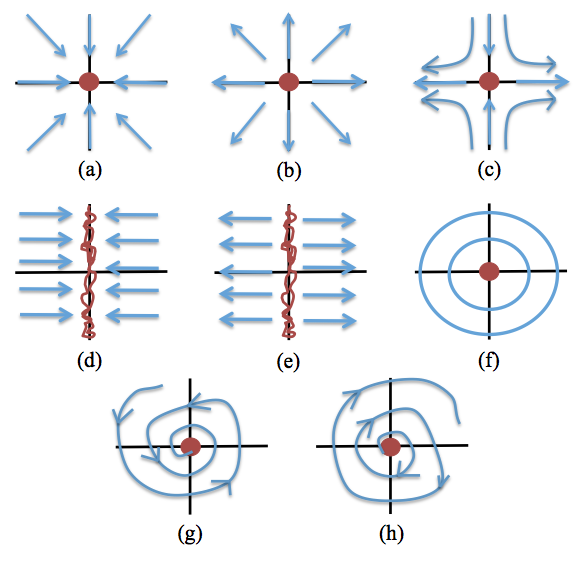
\includegraphics[width=5.0in]{EquilibriaClassification.png}
\caption{Various classifications of equilibrium based on eigenvalues of the Jacobian Matrix. (a) Sink (stable) Equilibrium (b) Source (unstable) Equilibrium (c) Saddle-Point Equilibrium (d) Degenerate Case 1 (e) Degenerate Case 2 (f) Center (g) Stable Foci (h) Unstable Foci}
\label{EquilibriaClassification}
\end{figure}

%
%
% Classifying Equilibria
%
% 
\begin{itemize}
%SINK
\item[ ] {\bf{Sink Equilibrium}}\\

In this case we assume two real eigenvalues, such that $\lambda_1,\lambda_2<0.$\\

 If we imagine finding a ``solution" to our linearized problem, e.g., $\frac{d {\bf{F}}({\bf{x}}_0}{dt} = J({\bf{x}}_0)({\bf{x-x}}_0).$, it is clear we will have the case of decaying exponentials in our diagonalization. Therefore we would assume any trajectory within a neighborhood of the equilibrium, ${\bf{x}}_0$, will head to the equilibria itself. Hence this case is known as a \emph{sink}. It is also stable. \\

This case can be seen in Figure(\ref{EquilibriaClassification})(a). \\

$ $\\


%SOURCE
\item[ ] {\bf{Source Equilibrium}}\\

In this case we assume two real eigenvalues, such that $\lambda_1,\lambda_2>0.$\\

Performing the same thought experiment as above, upon envisioning a solution the linearized problem, we find that any trajectory found within a neighborhood of the equilibrium would point away from the equilibria. Therefore this equilibria is known as a \emph{source}, as all trajectories point away from the equilibrium. It is also deemed unstable.\\

This case can be seen in Figure(\ref{EquilibriaClassification})(b).\\

$ $\\



%SADDLE-POINT
\item[ ] {\bf{Saddle-Point Equilibrium}}\\

In this case we assume two real eigenvalues, such that $\lambda_1>0,\lambda_2<0,$ hence one is positive and one is negative.\\

This case is called a \emph{saddle-point} equilibrium because some trajectories will be pointed towards the equilibria, while others will be pointed away. This is similar the idea of a saddle-point in multivariate calculus. Similarly in multivariate calulus, where a saddle-point is not strictly considered a local maxima or minima, it cannot be deemed either stable or unstable. \\

This case can be seen in Figure(\ref{EquilibriaClassification})(c). \\

$ $\\


%DEGENERATE CASES
\item[ ] {\bf{Degenerate Cases}}\\

In this case we assume two real eigenvalues, such that $\lambda_1\neq0,\lambda_2=0,$ hence one strictly zero and the other is real. In these type of degenerate cases, we will see bifurcated behavior. \\

For the case where $\lambda_1>0$, we believe solutions we act in a manner as seen in Figure(\ref{EquilibriaClassification})(d), while in the case where $\lambda_1<0$, the system has a feel of what is depicted in Figure(\ref{EquilibriaClassification})(e).\\

This type of behavior may be exhibited when radical structural differences occur in the trajectories when perturbing system parameters. \\

$ $\\


%CENETER
\item[ ] {\bf{Centers}}\\

In this case we assume two purely imaginary eigenvalues, such that $\lambda_1=bi,\lambda_2=-bi.$\\ Each trajectory around the equilibria, ${\bf{x}}_0$, is closed and circular in nature. This can be seen in Figure(\ref{EquilibriaClassification})(f). \\

We also note that if the Jaconian is \emph{skew-symmetric} at ${\bf{x}}={\bf{x}}_0$, then the equilbrium will always be a center, i.e., skew-symmetric matrices have purely imaginary eigenvalues. Let's actually do a quick proof.  

\begin{itemize}
\item[ ] {\bf{Proof}}: To show these trajectories are always circular, we begin with the relation that if $A=-A^*$, then the quadratic form $x^* A x = 0$. To prove this we can easily see that,

$$- x^* A x = x^* (-A) x = x^* A^* x = (x^* A x)^* = x^* A x,$$

since the quadratic form is a scalar quantity. Therefore we have $x^* A x = - x^* A x$ and hence $x^* A x = 0.$

Now that we have that relation, we consider the linearization, or actually just a linear system of ODEs,\\
$$\frac{d{\bf{x}}}{dt} = A {\bf{x}}.$$

Consider $A=-A^*$, and multiply the above by ${\bf{x}}^*$, \\

$${\bf{x}}^* \cdot \frac{d{\bf{x}}}{dt} = {\bf{x}}^* A {\bf{x}} = 0$$

Therefore we have \\

$${\bf{x}}^* \cdot \frac{d{\bf{x}}}{dt}  = \frac{1}{2} \frac{d}{dt} ( {\bf{x}}\cdot {\bf{x}} ) = \frac{d}{dt} ||x||^2 = 0.$$

From the above we get that all the orbits must be circular. \\

\end{itemize}

%\begin{Proof}
%To show a matrix has purely imaginary eigenvalues, we start with the \emph{Rayleigh Quotient},
%$$\lambda = \frac{{\bf{x}}^* A{\bf{x}}}{{\bf{x}}^*{\bf{x}}},$$
%%
%where $A\mathbb{R}^N$, ${\bf{x}}$ is our eigenvectors associated with eigenvalue, $\lambda$. Now we take the conjugate transpose (or conjapose...still not catching on? Okay, fine.) of the Rayleigh Quotient to get
%$$\lambda^* = \frac{ {\bf{x}}^* A* {\bf{x}} }{ {\bf{x}}^* {\bf{x}} } = \frac{ {\bf{x}}^* (-A) {\bf{x}} }{ {\bf{x}}^* {\bf{x}} } = -  \frac{ {\bf{x}}^* A {\bf{x}} }{ {\bf{x}}^* {\bf{x}} } = -\lambda.$$
%
%Hence we find that $\lambda^* = -\lambda$ and therefore we get that all eigenvalues must be purely imaginary. 
%\end{Proof}

$ $\\

%STABLE FOCUS
\item[ ] {\bf{Stable and Unstable Foci}}\\

In this case we assume two complex eigenvalues, such that $\lambda_1=a+bi,\lambda_2=a-bi,$ with $b\neq 0.$ \\ 

Depending on the sign of $a$, this system will either spiral towards or away from the equilbrium point. In both cases it will oscillate about the equilibrium with period $b$. Thinking of the solutions to the linearized problem, we note the stability will be controlled by if the solutions decay, i.e., $a<0$, or when they grow uncontrollably, i.e., $a>0.$ \\


For the case when $a<0$, the trajectories spiral towards the equilibria. We call the equilibrium a \emph{stable focus}.  Converging towards the equilibrium point is clear since the real part of the eigenvalue is negative. As in the \emph{sink} case, which also has negative real part, we expect trajectories to flow towards the equilibria. This can be seen in Figure(\ref{EquilibriaClassification})(g). \\

For the case when $a>0$, the trajectories spiral away from the equilibria. We call the equilibrium an \emph{unstable focus}. It is unstable since the real part of the eigenvalue is positive, and hence solutions should flow away from the equilibria, analogous to the \emph{source} case. This can be seen in Figure(\ref{EquilibriaClassification})(h). \\

\end{itemize}

In a neighborhood of the equilibria, we expect the solutions to behave like one of the above cases. Remember this is all \emph{local} analysis and at this junction cannot say anything about global solution behavior...yet  \\
\newpage
\graphicspath{{./Sturm_Liouville/}}

\section{Sturm Liouville Theory and Orthonogal Expansions!}

Sturm-Liouville theory regards second-order linear differential equations of the form

\begin{equation}
\label{SL_eq} \frac{d}{dx} \left[ p(x) \frac{dy}{dx} \right] + q(x) y = -\lambda w(x) y,
\end{equation} 

where $p(x), q(x)$, and $w(x)$ are  all continuous functions on the particular region of interest, say $[a,b]$. We also note that $w(x)>0$ and is referred to as the ``weight" function as well as that we assume $p(x)\in C^n$ with $n\geq 1$.\\

We further note that in this formalism we consider the solution $y(x)$ to obey boundary conditions on $[a,b]$. Moreover $\lambda$ is an eigenvalue of the our Sturm-Liouville operator and is chosen to give non-trivial solutions of (\ref{SL_eq}), which satisfy the boundary conditions.   \\

What makes Sturm-Liouville theory interesting and of particular use in applied mathematics is the factor that the linear differential operator given by (\ref{SL_eq}) is \emph{Hermitian} in some function space for specific boundary conditions.  What is special about \emph{Hermitian} operators is that their eigenfunctions are orthogonal (sometimes with the assistance of a weight function, i.e., $w(x)$) and form a complete function space. Recall how Hermitian operators work in Linear Algebra - they lead to a basis of orthogonal eigenvectors, each with real associated eigenvalue. \\


\begin{theorem}
\label{SL_theorem} If a Sturm-Liouville problem is \emph{regular}, i.e., if $p(x), p'(x), q(x),$ and $w(x)$ are all continuous on $[a,b]$ and have boundary conditions that can be written as 
\begin{align}
\label{SL_bcs} \alpha_1 y(a) + \alpha_2 y'(a) &= 0 \ \ \ \ \ \ with \ \ \ \ \ \alpha_1^2+\alpha^2>0 \\
\beta_1 y(b) + \beta_2 y'(b) &= 0 \ \ \ \ \ \ with \ \ \ \ \ \beta_1^2+\beta^2>0, 
\end{align}

then the eigenvalues of the Sturm-Liouville problem are real and can be ordered such that
$$\lambda_1 < \lambda_2 < \lambda_3 < \cdots < \lambda_n < \cdots \rightarrow \infty.$$
Furthermore with each eigenvalue, $\lambda_j$, there is a unique eigenfunction, $\phi_j(x)$, which has exactly $(j-1)$ roots in $(a,b)$, and with orthogonality property, i.e., 
$$\int_a^b \phi_j(x) \phi_k(x) w(x) dx =\left\{ \begin{array}{c} 
1,  \ \ \ \ j=k \\
0, \ \ \ \ j\neq k \end{array} \right.$$
\end{theorem}


\subsection{Application: Fourier Series and Orthogonal Series Expansions}

In this subsection we will explore where Fourier Series comes from, as well as, how to write an arbitrary continuous function, $f(x)$, in terms of Fourier Series. 

\subsubsection{Example: Fourier Sine Series}

Consider the following BVP, 
\begin{align}
y'' + \lambda y &= 0 \\ 
y(0) &= 0 \\
y(1) & = 0.
\end{align}

Now we have three cases to consider:
\begin{enumerate}
\item $\lambda = 0$
\item $\lambda = -\alpha^2 < 0$
\item $\lambda = \alpha^2 > 0$
\end{enumerate}

\begin{itemize}
\item[Case 1: ] $\lambda = 0$: We have the following ODE to solve $$y'' = 0$$ and hence we obtain $$y(x) = c_1 + c_2 x.$$
Inserting the boundary conditions, we see that $c_1 = c_2 = 0$, and hence we only have the trivial solution in this case. 

\item[Case 2: ] $\lambda = -\alpha^2 < 0:$ We have the following ODE to solve $$y'' - \alpha^2 y = 0.$$  We find the general solution of $$y(x) = c_1 \sinh(\alpha x) + c_2 \cosh(\alpha x).$$

Using the boundary conditions we see
\begin{align*}
y(0)=0 &\Rightarrow c_2 = 0 \\
y(1)=0 &\Rightarrow c_1 \sinh(\alpha) = 0 \Rightarrow c_1 = 0. 
\end{align*}

Hence we only have the trivial solution, once again.

\item[Case 3: ] $\lambda = \alpha^2 > 0$: We consider the following ODE, $$y''+\alpha^2 y= 0,$$ where $\alpha^2>0$. We find the general solution to be

$$y(x) = c_1 \sin(\alpha x) + c_2 \cos(\alpha x).$$

Using the boundary conditions we see
\begin{align*}
y(0)=0 &\Rightarrow c_2 = 0 \\
y(1)=0 &\Rightarrow c_1 \sin(\alpha) = 0 \Rightarrow \alpha = n\pi \ \ \ \mbox{where}\ n\in\mathbb{Z}^{+}. 
\end{align*}

Therefore we find our eigenvalues to be $\lambda_n = \alpha_n^2 = n^2\pi^2,$ for $n\in\mathbb{Z}^{+}$, with associated eigenfunctions, $\phi_n(x) = \sin(n\pi x).$
%


We will now demonstrate the orthogonality of those eigenfunctions.

\item[Orthogonality: ]

Consider $$\int_0^1 \sin(n\pi x) \sin(m \pi x) dx,$$

where $n\neq m.$ Now we use the following identity to perform the integration,

$$\sin(a)\sin(b) = \frac{1}{2} \Big[ \cos(a-b) - \cos(a+b) \Big].$$

\begin{align*}
\int_0^1 \sin(n\pi x) \sin(m \pi x) dx &= \int_0^1   \frac{1}{2} \Big[ \cos( (n-m)\pi x) - \cos( (n+m)\pi x) \Big]  dx \\
%
&= \frac{1}{2} \Big[ \frac{1}{(n-m)\pi}  \sin( (n-m)\pi x) - \frac{1}{(n+m)\pi}  \sin( (n+m)\pi x)  \Big]_0^1 \\
%
&= 0.
\end{align*}

We note that the case $n=m$ must be considered by itself, to avoid singularity in the above integration. Moreover, the case where $n=m=0$ is disgarded since $0$ is not an eigenvalue of the differential operator. Now we show the case $n=m\neq 0$ leads to a non-zero computation. 

Now considering $n=m\neq 0$,

\begin{align*}
\int_0^1 \sin^2(n\pi x)dx &= \frac{1}{2} \int_0^1\Big[1 - \cos(2n\pi x)\Big] dx \\
%
&= \frac{1}{2} \Big[x - \frac{1}{2n\pi} \sin(2n\pi x) ]_0^1 \\
%
&= \frac{1}{2}.
\end{align*}

Hence orthogonality holds (as it should)!

\end{itemize}


%
%
% FOURIER SERIES EXAMPLE!
%
%
\subsubsection{Example: Fourier Series of a function $f(x)$}

Now we will illustrate how to use this idea of Fourier Series in rewriting a function, $f(x)$. First we begin with the general form of a Fourier Series. Written as an infinite sum, a Fourier Series of a function $f(x)$ on an interval $[-L,L]$ is written as,

\begin{equation}
\label{fourier_series} f(x) = \sum_{j=0}^{\infty} a_j \cos\left( \frac{j\pi x}{L} \right ) +  \sum_{j=1}^{\infty} b_j \sin\left( \frac{j\pi x}{L} \right ).
\end{equation}

The brunt of the work is now calculating the coefficients $\{a_n\}_{n=0}^{\infty}$ and $\{b_n\}_{n=1}^{\infty}$. Luckily we can employ orthogonality properties of the Fourier eigenfunctions.

\begin{align}
\int_{-L}^L \cos\left( \frac{n\pi x}{L} \right ) \cos\left( \frac{m\pi x}{L}\right) dx &=\left\{\begin{array}{c}2L\ \ \ \ n=m=0 \\ L \ \ \ \ n=m>0 \\ 0 \ \ \ \ n\neq m \end{array}\right. \\
\int_{-L}^L \sin\left( \frac{n\pi x}{L} \right ) \sin\left( \frac{m\pi x}{L} \right) dx &= \left\{\begin{array}{c} L \ \ \ \ n=m>0 \\ 0 \ \ \ \ n\neq m \end{array}\right. \\
\int_{-L}^L \sin\left( \frac{n\pi x}{L} \right ) \cos\left( \frac{m\pi x}{L} \right) dx &= 0.
\end{align}

To compute the coefficients, we begin with (\ref{fourier_series}) and multiply by either eigenfunction. First let's consider the contributions by the $\Big\{  \sin\left( \frac{n\pi x}{L} \right ) \Big\}$ eigenfunctions in the expansion of $f(x)$. We begin with

$$f(x) = \sum_{n=0}^{\infty} a_n \cos\left( \frac{n\pi x}{L} \right ) +  \sum_{n=1}^{\infty} b_n \sin\left( \frac{n\pi x}{L} \right ),$$

and multiply both sides by $\sin\left( \frac{m\pi x}{L} \right )$. Next we integrate both sides over the interval of interest, e.g.,

$$\int_{-L}^L f(x) \sin\left( \frac{m\pi x}{L} \right )  dx=\int_{-L}^{L}\Bigg[ \sum_{n=0}^{\infty} a_n \cos\left( \frac{n\pi x}{L} \right ) +  \sum_{n=1}^{\infty} b_n \sin\left( \frac{n\pi x}{L} \right ) \Bigg] \sin\left( \frac{m\pi x}{L} \right ) dx.$$

The only terms that are not zero in the above equation, are those for which $n=m$ and the sinusoidal terms, i.e.,

$$\int_{-L}^L f(x) \sin\left( \frac{m\pi x}{L} \right )  dx = \int_{-L}^{L} b_m \sin^2\left( \frac{m\pi x}{L} \right ) dx.$$

Hence since $b_m$ is a constant, we can solve for it to get

$$b_m = \frac{ \int_{-L}^L f(x) \sin\left( \frac{m\pi x}{L} \right )  dx }{  \int_{-L}^{L} \sin^2\left( \frac{m\pi x}{L} \right ) dx }.$$

Therefore we now have a formula to find all the coefficients $\{b_j\}_{j=1}^{\infty}.$ Using a similar approach and employing orthogonality once again, we can find a formula for the $\{a_j\}_{j=0}^{\infty}$ coefficients as well, i.e., 

$$a_m = \frac{ \int_{-L}^L f(x) \cos\left( \frac{m\pi x}{L} \right )  dx }{  \int_{-L}^{L} \cos^2\left( \frac{m\pi x}{L} \right ) dx }.$$

After computing all those integrals, we will have our expansion of $f(x)$ on $[-L,L]$ in all its Fourier Series glory!


%
%
% FOURIER SERIES OF f(x) = x
%
%
\subsubsection{Example: Fourier Series of $f(x)=x$ on $[-\pi,\pi]$}

We wish to find $$f(x) = x = \sum_{j=0}^{\infty} a_j \cos(jx)+  \sum_{j=1}^{\infty} b_j \sin(jx).$$

Welp, let's do the integrals!

\begin{align*}
b_m &= \frac{ \int_{-\pi}^{\pi} x \sin(mx) dx }{  \int_{-\pi}^{\pi} \sin^2(mx) dx }. \\
&= \frac{ -\frac{x}{m}\cos(mx) \Big|_{-\pi}^{\pi} + \frac{1}{m}\int_{-\pi}^{\pi} \cos(mx) dx }{\pi} \\
&= \frac{ \frac{-2\pi}{m} cos(m\pi) }{\pi} \\
& = \frac{2}{m} (-1)^{m+1}
\end{align*}

Similarly, we'll consider the integrations to find $\{ a_n \}$. Let's start with $m>0$,
\begin{align*}
a_m &= \frac{ \int_{-\pi}^{\pi} x \cos(mx) dx }{  \int_{-\pi}^{\pi} \cos^2(mx) dx }. \\
&= \frac{ \frac{x}{m}\sin(mx) \Big|_{-\pi}^{\pi} - \frac{1}{m}\int_{-\pi}^{\pi} \sin(mx) dx }{\pi} \\
&= 0
\end{align*}

and when $m=0$ for $a_0$,

$$a_0 = \frac{ \int_{-\pi}^{\pi} x dx }{ \int_{-\pi}^{\pi} 1 dx } = 0.$$

Therefore all the cosines drop out of our Fourier Expansion of $f(x)=x$ on $[-\pi,\pi].$ Note, we could have easily seen this by the fact the function we are rewriting in the Fourier basis, $f(x)=x$, is odd on a symmetric interval.  We then have

$$f(x) = x = \sum_{m=1}^{\infty} \left[ \frac{2}{m} (-1)^{m+1}\right] \sin(mx).$$

The figure below shows what the Fourier Series expansion looks like on that interval for differing number of terms in the series.

\begin{center}
\begin{figure}[h!]
 	\centering
  	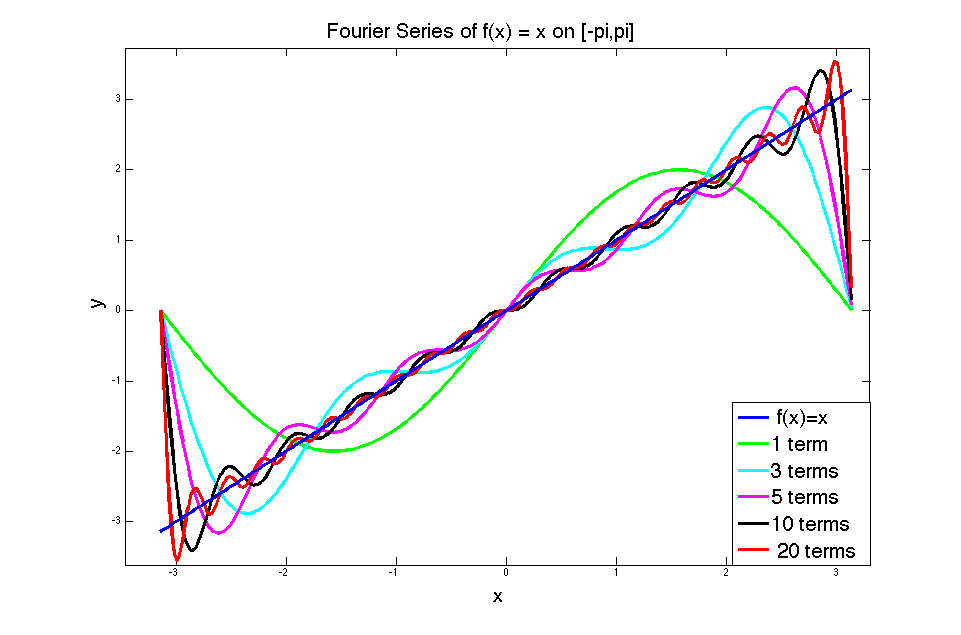
\includegraphics[scale=0.5]{Fourier_Series_Ex.png}
 	\caption{The function $f(x)=x$ being expressed as Fourier Series expansions with differing numbers of truncated terms.}
 	\label{Fourier_Series_Ex}
\end{figure}
\end{center}


%
%
% GENERAL ORTHOGONAL EXPANSIONS
%
%

\subsection{General Orthogonal Series Expansions}

As we saw in the above example, we can express a function $f(x)$ in terms of sines and cosines on a specified interval. We recall we are able to do this because the those sines and cosines, i.e., $\left\{ \cos\left( \frac{j\pi x}{L} \right ) \right\}$ and $\left\{ \cos\left( \frac{j\pi x}{L} \right ) \right\}$, on $[-L,L]$ form a complete basis in function space. Moreover, these functions were eigenfunctions of a Sturm-Liouville differential operator, so we knew we were guaranteed those properties - namely orthogonality and completeness. \\

Beyond Fourier Series there are many ``popular" orthogonal polynomials, which are all eigenfunctions of some Sturm-Liouville differential operator. Just for some buzzwords, the usual candidates tend to be:

\begin{itemize}
\item Bessel Functions
\item Chebyshev Polynomials
\item Legendre Polynomials
\item Laguerre Polynomials
\item Hermite Polynomials
\end{itemize}

More generally, if $\left\{ \phi_j(x) \right\}$ are eigenfunctions of a Sturm-Liouville problem, and we wish to expand some function $f(x)$ on an interval $[a,b]$ in terms of them, i.e., 
$$f(x) = \sum_{j=0}^{\infty} c_j \tilde{\phi}_j(x),$$

the brunt of the work still lies in calculating the coefficients $\{ c_j\}$. We note that $\tilde{\phi}_j(x)$ are the eigenfunctions, $\phi_j(x)$, just translated into the interval $[a,b].$ We can do the same procedure as we did to find the Fourier Series coefficients. Let's party!

\begin{align*}
f(x) &= \sum_{m=0}^{\infty} c_m \tilde{\phi}_m(x) \\
 f(x) \tilde{\phi}_n(x)  &=\sum_{m=0}^{\infty} c_m \tilde{\phi}_m(x) \tilde{\phi}_n(x)  \\
  f(x) \tilde{\phi}_n(x) \tilde{w}(x)  &=\sum_{m=0}^{\infty} c_m \tilde{\phi}_m(x) \tilde{\phi}_n(x) \tilde{w}(x) \\
\int_{a}^{b} f(x) \tilde{\phi}_n(x) \tilde{w}(x) dx &= \int_a^b \sum_{m=0}^{\infty} c_m \tilde{\phi}_m(x) \tilde{\phi}_n(x) \tilde{w}(x) dx \\
\int_{a}^{b} f(x) \tilde{\phi}_n(x) \tilde{w}(x) dx &= \sum_{m=0}^{\infty} c_m  \int_a^b  \tilde{\phi}_m(x) \tilde{\phi}_n(x)  \tilde{w}(x) dx \\
\int_{a}^{b} f(x) \tilde{\phi}_n(x) \tilde{w}(x) dx &=  c_n \int_a^b  \tilde{\phi}^2_n(x) \tilde{w}(x) dx \\
\end{align*}

and hence we obtain

$$c_n = \frac{  \int_{a}^{b} f(x) \tilde{\phi}_n(x) \tilde{w}(x) dx    } { \int_a^b  \tilde{\phi}^2_n(x) \tilde{w}(x) dx  }.$$

Note: $\tilde{w}(x)$ is the weight function that comes from (\ref{SL_eq}), just translated into the appropriate interval $[a,b]$.


%
%
% SOLVING ODEs WITH FOURIER SERIES!
%
%
\subsection{Using Fourier Series to Solve ODEs}

Consider the following $2^{nd}$ order linear constant-coefficient ODE:

$$\hat{L}u = \alpha u'' + \beta u' + \gamma u = g(x),$$

where $\{\alpha, \beta, \gamma\}\in\mathbb{R}$, $u=u(t)$ and and either Dirichlet, Neumann, or mixed type  boundary conditions, on some interval $[-L,L]$. If the ODE is not defined on such an interval, simply do a transformation into it. We then must solve for both the complementary solution, $u_C(x)$, i.e., the solution to the homogeneous problem, as well as the particular solution, $u_P(x)$, e.g., the solution to the non-homogeneous problem. Our full solution will be of the form $$u(x) = u_C(x) + u_P(x).$$

Now in doing the above we will employ the services of Fourier Series to find the particular solution, $u_P(x).$ We note that if $g(x)$ is a fairly simple function, e.g., a polynomial, sine, cosine, or exponential, or even products of them, finding the particular solution using \emph{undetermined coefficients} is probably the road more traveled (and it should be). If $g(x)$ is not a simple function like those, you can try to use \emph{variation of parameters}; however, if you do not know the complementary solutions, this could prove rather difficult. Now if $g(x)$ is periodic with period $2L$, this is where Fourier Series can come in!

 We wish to write our solution $u_P(x)$ in a Fourier Series, 

$$u_P(x) =  \sum_{j=0}^{\infty} a_j \cos\left( \frac{j\pi x}{L} \right ) +  \sum_{j=1}^{\infty} b_j \sin\left( \frac{j\pi x}{L} \right ).$$

However, first we must also expand $g(x)$ in its Fourier Series, e.g.,

$$g(x) =  \sum_{j=0}^{\infty} c_j \cos\left( \frac{j\pi x}{L} \right ) +  \sum_{j=1}^{\infty} d_j \sin\left( \frac{j\pi x}{L} \right );$$

however, since $g(x)$ is a known function we can find the coefficients $\{ c_j \}$ and $\{ d_j \}$ explicitly using the methods above. We now have a  linear differential equation of the form,

$$\hat{L}u = \sum_{j=0}^{\infty} c_j \cos\left( \frac{j\pi x}{L} \right ) +  \sum_{j=1}^{\infty} d_j \sin\left( \frac{j\pi x}{L} \right ).$$

Substituting our solution ansatz (the Fourier Series for $x_P(x)$) into the equation above, we see we get

\begin{align*}
\hat{L}u &= g(x) \\ \\
\hat{L}u &= \sum_{j=0}^{\infty} c_j \cos\left( \frac{j\pi x}{L} \right ) +  \sum_{j=1}^{\infty} d_j \sin\left( \frac{j\pi x}{L} \right ) \\ \\
\hat{L} \left[   \sum_{j=0}^{\infty} a_j \cos\left( \frac{j\pi x}{L} \right ) +  \sum_{j=1}^{\infty} b_j \sin\left( \frac{j\pi x}{L} \right ) \right]  &= \sum_{j=0}^{\infty} c_j \cos\left( \frac{j\pi x}{L} \right ) +  \sum_{j=1}^{\infty} d_j \sin\left( \frac{j\pi x}{L} \right ) \\ \\
 \sum_{j=0}^{\infty} a_j \hat{L} \left[ \cos\left( \frac{j\pi x}{L} \right ) \right] + \sum_{j=1}^{\infty} b_j \hat{L}\left[ \sin\left( \frac{j\pi x}{L} \right ) \right] &= \sum_{j=0}^{\infty} c_j \cos\left( \frac{j\pi x}{L} \right ) +  \sum_{j=1}^{\infty} d_j \sin\left( \frac{j\pi x}{L} \right ) \\ 
\end{align*}


What is left is to write a system of equations for all the $\{a_j\}$ and $\{b_j\}$ coefficients in terms of $\{ c_j\}$ and $\{d_j\}$. Note that if the damping term in not present in the ODE, i.e., $\beta=0$, there is the possibility of the presence of resonance, so the corresponding frequency term must include a polynomial type coefficient, $i.e., x$, as well.\\  

Furthermore we note that if we have Dirichlet boundary conditions, we will use a Fourier Sine Series for both $g(x)$ and $y_P(x)$, if Neumann, we will use the Fourier Cosine Series for them. 






%%%%%%%%%%%%%%%%%%%%%%%%%%%%%%%%%%
%
%
% GRAM SCHMIDT
%
%
%%%%%%%%%%%%%%%%%%%%%%%%%%%%%%%%%%

\subsection{Gram-Schmidt Processes...for othogonal polynomials?!}

If you're ever in a situation where you need to know the first few othogonal polynomials in a particular basis family, have no fear! You can derive them using a Gram-Schmidt process. That's right - just like in linear algebra. \emph{Note} that you can derive as many as you wish using this methodology...if you have enough time and mental arithmetic fortitude. \\

Before we proceed with Gram-Schmidt for othogonal polynomials we first recall the Gram-Schmidt process for othogonalizing vectors in $\mathbb{R}^n$. Once we have reviewed this, the leap to Gram-Schmidt processes for infinitely dimensinoal functional spaces will feel like a natural extension.


%
%
% GRAM-SCHMIDT FOR VECTORS IN R^n
%
%
\subsubsection{Gram-Schmidt for vectors in $\mathbb{R}^n$}

Consider a set of m-vectors in $\mathbb{R}^n$, with $m\leq n$, $\{ {\bf{v}}_1, {\bf{v}}_2, {\bf{v}}_3, \ldots, {\bf{v}}_m\}$. In general when handed a set of vectors, they will not be orthogonal; however, we will employ the services of Gram-Schmidt to help us achieve this feat. In order for the Gram-Schmidt process to achieve a set of m-orthogonal vectors from a collection of vectors, all the vectors must be linearly independent. We note that the span of the original vector space and that of the orthogonalized vector space are equivalent. 

To orthogonalize a collection of vectors, we begin with a single vector, say ${\bf{q}}_1={\bf{v}}_1$. Next we proceed to find an orthogonal vector to ${\bf{q}}_1$, by taking ${\bf{v}}_2$ and subtracting off the projection of ${\bf{v}}_2$ onto ${\bf{q}}_1$. To find the next orthogonal vector, we will repeat this process and take ${\bf{v}}_3$ and subtract off the projections of ${\bf{v}}_3$ onto ${\bf{v}}_1$ and ${\bf{q}}_2$. This process is illustrated below.

\begin{align*}
{\bf{q}}_1 &= {\bf{v}}_1 \\ 
{\bf{q}}_2 &= {\bf{v}}_2 - proj_{ {\bf{q}}_1 } {\bf{v}}_2 \\
{\bf{q}}_3 &= {\bf{v}}_3 - proj_{ {\bf{q}}_1 } {\bf{v}}_3  - proj_{ {\bf{q}}_2} {\bf{v}}_3\\ 
{\bf{q}}_4 &= {\bf{v}}_4 - proj_{ {\bf{q}}_1 } {\bf{v}}_4  - proj_{ {\bf{q}}_2} {\bf{v}}_4 - proj_{ {\bf{q}}_3} {\bf{v}}_4 \\ 
& \vdots  \\ 
{\bf{q}}_m &=  {\bf{v}}_m - \sum_{k=1}^{m-1} proj_{ {\bf{q}}_k }   {\bf{v}}_m.
\end{align*}

We now recall the strict definition of a vector projection. The projection of a vector ${\bf{v}}$ onto a vector ${\bf{u}}$ is defined as

 $$proj_{{\bf{u}}} {\bf{v}}= \frac{< {\bf{v}} , {\bf{u}}> }{ < {\bf{u}} , {\bf{u}} >  } {\bf{u}}, $$ 

$<\cdot, \cdot>$ is an inner-product.

Hence we can rewrite the Gram-Schmidt process in terms  of inner-products, e.g.,

\begin{align*}
{\bf{q}}_1 &= {\bf{v}}_1 \\ 
{\bf{q}}_2 &= {\bf{v}}_2 -  \frac{< {\bf{v}}_2 , {\bf{q}}_1 > }{ < {\bf{q}}_1 , {\bf{q}}_1 >  } {\bf{q}}_1 \\
{\bf{q}}_3 &= {\bf{v}}_3 - \frac{< {\bf{v}}_3 , {\bf{q}}_1 > }{ < {\bf{q}}_1 , {\bf{q}}_1 >  } {\bf{q}}_1  - \frac{< {\bf{v}}_3 , {\bf{q}}_2 > }{ < {\bf{q}}_2 , {\bf{q}}_2 >  } {\bf{q}}_2\\ 
{\bf{q}}_4 &= {\bf{v}}_4 - \frac{< {\bf{v}}_4 , {\bf{q}}_1 > }{ < {\bf{q}}_1 , {\bf{q}}_1 >  } {\bf{q}}_1  -  \frac{< {\bf{v}}_4 , {\bf{q}}_2 > }{ < {\bf{q}}_2 , {\bf{q}}_2>  } {\bf{q}}_2 - \frac{< {\bf{v}}_4 , {\bf{q}}_3 > }{ < {\bf{q}}_3 , {\bf{q}}_3 >  } {\bf{q}}_3 \\ 
& \vdots  \\ 
{\bf{q}}_m &=  {\bf{v}}_m - \sum_{k=1}^{m-1}  \frac{< {\bf{v}}_m , {\bf{q}}_k > }{ < {\bf{q}}_k , {\bf{q}}_k >  } {\bf{q}}_k.
\end{align*}

The last thing we can do is normalize these newly found orthogonal vectors, $\{ {\bf{q}}_1, {\bf{q}}_2, \ldots, {\bf{q}}_m \}$, using the standard normalization procedure, e.g., 
$$\{ \hat{{\bf{q}}}_1, \hat{{\bf{q}}}_2, \ldots, \hat{{\bf{q}}}_m \} = \Bigg\{ \frac{ {\bf{q}}_1 }{|| {\bf{q}}_1 || },  \frac{ {\bf{q}}_2 }{|| {\bf{q}}_2 || }, \ldots,  \frac{ {\bf{q}}_m }{|| {\bf{q}}_m || } \Bigg\},$$

where $\hat{ {\bf{q}}}_k$ is now orthonormalized.  


%
%
% GRAM-SCHMIDT FOR POLYS
%
%
\subsubsection{Gram-Schmidt for Orthogonal Polynomials!}

We now shift gears slightly and look to the problem of creating a basis of orthogonal polynomials. We recall if two polynomials, say $p_k$ and$p_j$ are orthogonal then we have 

$$<p_k, p_j> = \int_{a}^{b} p_k(x) p_j(x) w(x) dx = \left\{ \begin{array}{c} 0 \ \ \ (j\neq k) \\ c\in\mathbb{R} \ \ \ (j=k)  \end{array} \right. ,$$
%
where $w(x)$ is a weight-function associated with the specific orthogonal polynomials behind the scenes Sturm-Liouville problem. On that note, we point out that in order to easily extend Gram-Schmidt from vectors in $\mathbb{R}^n$ to infinite dimensional function space, we need to define an inner-product. We do so accordingly,

$$<p_k, p_j> = \int_{a}^{b} p_k(x) p_j(x) w(x) dx.$$

For constructing families of orthogonal polynomials, we will use the above inner-product and see that any family of orthogonal polynomials is going to be generated by changing the weight function, $w(x)$, in the above inner-product. For examples, to construct the \emph{Legendre} polynomial basis we use $w(x)=1$, while for \emph{Chebyshev} polynomials the weight function is $w(x) = \frac{1}{\sqrt{1-x^2}}.$ We also need correct integration bounds, i.e., for both Legendre and Chebyshev polynomails we need $[a,b]=[-1,1].$\\

To construct the orthogonal basis of polynomials we proceed in a similar manner to the above, except starting off with $p_0=1$ as the zero-th order polynomial. To find $p_1(x)$, the $1^{st}$-order orthogonal polynomial, we subtract off the projection of the $1^{st}$-order monomial basis function onto $p_0(x)$ from $x$. We then continue in an analogous manner. The procedure can be seen as 

\begin{align*}
p_0(x) &= 1 \\
p_1(x) &= x - \frac{ < x, p_0>  }{ <p_0, p_0>  } p_0(x) \\
p_2(x) &= x^2 - \frac{ < x^2 , p_0>  }{ <p_0, p_0>  } p_0(x) -  \frac{ < x^2 , p_1>  }{ <p_1, p_1>  } p_1(x) \\
p_3(x) &= x^3 - \frac{ < x^3 , p_0>  }{ <p_0, p_0>  } p_0(x) -  \frac{ < x^3 , p_1>  }{ <p_1, p_1>  } p_1(x) -  \frac{ < x^3 , p_2>  }{ <p_2, p_2>  } p_2(x)  \\
&\vdots \\
p_n(x) &= x^n  - \sum_{k=0}^{n-1} \frac{ < x^n , p_k>  }{ <p_k, p_k>  } p_k(x). \\
\end{align*}

It is clear that doing this procedure is definitely not optimal, especially if you need to find $p_{10}(x)$, or even $p_3(x)$ for that matter. However, where this procedure becomes powerful is in the realm of numerical quadrature, or numerical integration. In a nutshell, in the Gaussian quadrature formulation of approximating integrals, one needs to (*gets to) choose \emph{both} the quadrature points as well as the weight coefficients. It turns out that one possible method for choosing the quadrature becomes is naturally found to be constructing a specific family of orthogonal polynomials and then finding the roots of the desired order, e.g., if we wish to find $2$ quadrature nodes, we would find the roots of $p_2(x)$.\\

 Furthermore because of the accuracy of Gaussian Quadrature compared to Newton-Cotes methods, where the only degrees of freedom are the weight coefficients, as the quadrature points are known \emph{a priori.}, one only needs to construct polynomials of modest order. The main difference between the two numerical integrations methods can be seen as having $2N$ degrees of freedom in Gaussian Quadrature, while only $N$ degrees of freedom in Newton-Cotes. These degrees of freedom have immediate consequence in eliminating lower order errors to achieve higher order accuracy.

%
%We will illustrate this with an example.
%
%\begin{itemize}
%
%\item[] {\bf{Example}}: Consider the following ODE: $y'' + 3y = x$ with $y(-\pi)=y(\pi)=0.$\\
%
%Luckily we have computed the Fourier Series for $g(x)=x$ on $[\pi,\pi]$ above, and found it to be: $$g(x) = x = \sum_{m=1}^{\infty} \left[ \frac{2}{m} (-1)^{m+1}\right] \sin(mx).$$
%
%Rolling through the rigmarole describe above we first assume a solution of the form $$u(x) = \sum_{j=0}^{\infty} a_j \cos(jx)+  \sum_{j=1}^{\infty} b_j \sin(jx).$$
%
%Substituting this into the ODE we get
%$$y''+3y =  \sum_{m=0}^{\infty} (3-m^2) a_m \cos(mx) +  \sum_{m=1}^{\infty} (3-m^2) b_m \sin(mx) =\sum_{m=1}^{\infty} \left[ \frac{2}{m} (-1)^{m+1}\right] \sin(mx) = g(x).$$
%
%and hence we need that 
%\begin{align*}
%(3-m^2) a_m &= 0  \\
%(3-m^2) b_m &= \frac{2}{m} (-1)^{m+1}. \\
%\end{align*}
%
%Therefore we get that $$b_m = \frac{2}{m(3-m^2)} (-1)^{m+1},$$
%
%and we get that our solution is: $$u(x) = \sum_{m=1}^{\infty} \left[ \frac{2}{m(3-m^2)} (-1)^{m+1} \right] \sin(mx).$$
%
%
%\end{itemize}
\newpage
\graphicspath{{./Greens_Function/}}

\section{Green's Function}

A Green's function, denoted $G(x,s)$, is associated with specific linear differential operator, $\hat{L}$. It is the solution to 
\begin{equation}
\label{Greens_Def} \hat{L}G(x,s) = \delta(x-s),
\end{equation}

where $\delta(x-s)$ is the Dirac-delta function. As applied mathematicians we wish to exploit properties of the Green's function that makes them particularly useful for solving non-homogeneous differential equations, whether they are of the \emph{ordinary} or \emph{partial} varieties, e.g., Green's functions can be used for finding solutions to equations of the form
\begin{equation}
\label{bvp_ode} \hat{L} u(x) = f(x),
\end{equation}

where $u(x)$ is the solution we seek and $\hat{L}$ is some differential operator. Specifically we will use them to solve non-homogeneous boundary value problems (BVPs). We note that BVPs sometimes do not have solutions, so we will illustrate the main concepts of Green's Function using ``nice" linear differential operators. 

\subsection{Big Picture of Green's Functions}

We consider $L$ to be of the Sturm-Liouville family of differential operators, i.e., 
\begin{equation}
\label{sturm_liouville_op} \hat{L} = \frac{d}{dx} \left( p(x) \frac{d}{dx} \right) + q(x),
\end{equation}

where we presume $p(x)$ and $q(x)$ are continuous functions on some interval of interest, say $[a,b]$. Naturally, we have some boundary conditions, written in the form,
\begin{equation}
\hat{D}u = \left\{ \begin{array}{c}
c_1 u'(a)+c_2 u(a) = 0 \\
c_3 u'(b) + c_4 u(b) = 0.
\end{array}\right.
\end{equation}

Note: we call the operator $\hat{D}$, the \emph{boundary conditions operator}. (very creatively, in fact). 

We consider the following BVP,
\begin{equation}
\label{BVP} \hat{L}u(x) = f(x)  \ \ \ \  w/ \ \ \ \  \hat{D} u = 0,
\end{equation}

where $f(x)$ is continuous on $[a,b]$. We can induce there is only one solution to the above BVP, given by 
\begin{equation}
\label{greens_solution} u(x) = \int_a^b G(x,s) f(x) ds.
\end{equation}

The name of the game will then be constructing the appropriate Green's function for the specific linear differential operator. It is clear once we have the Green's function, we can change the non-homogeneous term in the BVP, i.e., $f(x)$, and assuming our integration skills are up to it, find the solution $u(x)$ to our BVP.

\subsection{Properties of Green's Functions}

Green's functions have the following properties:
\begin{itemize}
\item $G(x,s)$ is \emph{continuous} in $x$ and $s$
\item For $x\neq s$, $\hat{L}G(x,s) = 0.$
\item For $s\neq 0$, $\hat{D} G(x,s) = 0.$
\item Symmetry Condition: $G(x,s) = G(s,x)$.
\item Jump Discontinuity: $G'(s_{+},s) - G'(s_{-},s) = \frac{1}{p(s)}.$
\end{itemize}

{\bf{Note:}} Many of our friendly linear differential operators already have had their Green's functions found and studied extensively! Look them up and then have an integration party!

\subsection{A little motivation...}

Consider the following integral with Dirac-delta kernel, 
\begin{equation}
\label{delta_integral} \int_a^b f(s) \delta(x-s) ds.
\end{equation}

We know by properties of the Dirac-delta function that this integral is equal to
$$\int_a^b f(s) \delta(x-s) ds = f(x)$$.

Now recall (\ref{Greens_Def}) and substituting this into the above equation gives,
$$\int_a^b f(s) \delta(x-s) ds = \int_a^b \hat{L} G(x,s) f(s) ds  =  f(x),$$

and by (\ref{bvp_ode}), we obtain

$$\hat{L}u(x) = \int_a^b \hat{L} G(x,s) f(s) ds .$$

Finally by uniform convergence (and other analysis theorems, we take for granted, but never should), but moreso we simply note that $\hat{L}$ is only a differential operator on $x$, and hence can be pulled out of the integrand, e.g.,

$$\hat{L}u(x) = \hat{L} \left( \int_a^b  G(x,s) f(s) \right),$$

which strongly infers that we obtain our solution of
\begin{equation}
u(x) = \int_a^b G(x,s) f(s) ds.
\end{equation}


\subsection{Example: u'' + 4u = f(x) }

Consider the following BVP w/ associated boundary conditions,

\begin{align}
u'' + 4u &= f(x) \\
u(0) &= 0 \\
u\left(  frac{\pi}{4} \right)  &= 0.
\end{align}

We now proceed in finding the Green's Function for the operator $\hat{L} = \frac{d^2}{dx^2} + 4.$ We begin by first solving the following ODE with respect to the Green's function, $G$,

$$G'' + 4G = \delta(x-s),$$

where we will have to consider two regions:
\begin{enumerate}
\item $0\leq x\leq s$
\item $s\leq x \leq \frac{\pi}{4}$
\end{enumerate}

Now we get from simple ODE theory that
$$G(x,s) = c_1 \cos(2x) + c_2 \sin(2x)$$
where coefficients $c_1$ and $c_2$ will depend on $s$.

Looking into the boundary conditions on each region appropriately, we see that for:
\begin{enumerate}
\item $x\in [0,s] : G(0,s) = 0 \Rightarrow c_1(s) = 0$
\item $x\in [s,frac{\pi}{4}] : G\left(\frac{\pi}{4},s\right) = 0 \Rightarrow c_2(s) = 0$
\end{enumerate}

Therefore we find that 
$$G(x,s) = \left\{ \begin{array}{c}
c_2(s) \sin(2x)  \ \ \ \ \  x\in[0,s], \\
c_1(s) \cos(2x) \ \ \ \ \  x\in[s,\frac{\pi}{4}].
\end{array} \right. $$

Now we must find the functional forms of $c_1(s)$ and $c_2(s)$. We will be able to do this by using the fact we need $G(x,s)$ to be continuous in \emph{both} $x$ and $s$, as well as the \emph{jump discontinuity} in the derivative of $G(x,s)$.

First we will look at continuity. 
\begin{itemize}
\item[Continuity]: We need that $G(x,s)$ has the same limit as $x\rightarrow s$ from below and $x\rightarrow s$ from above.

This gives us that
\begin{equation}
\label{continuity_eq1} c_2(s) \sin(2s) = c_1(s) \cos(2s).
\end{equation}

\item[Jump]:  $\lim_{\epsilon\rightarrow0} \left[ \frac{dG}{dx}\Bigg|_{s+\epsilon} -  \frac{dG}{dx}\Bigg|_{s-\epsilon}   \right] = \frac{1}{p(x)}$.

We note that $p(x)$ = 1 for our toy problem. We find that
\begin{equation}
\label{jump_discontinuity} -2c_1(s) \sin(2s) - 2c_2(s) \cos(2s) = 1.
\end{equation}

\end{itemize}

Now solving (\ref{continuity_eq1}) and (\ref{jump_discontinuity}) for $c_1(s)$ and $c_2(s)$, we find
\begin{align}
c_1(s) &= -\frac{1}{2}\cos(2s)  \\
c_2(s) &= \frac{1}{2}\sin(2s),
\end{align}

and hence we find our Green's function to be:
\begin{equation}
\label{Green_example_sol} G(x,s) = \left\{ \begin{array}{c}
-\frac{1}{2} \cos(2s) \sin(2x) \ \ \ \ \ x\in[0,s] \\
-\frac{1}{2}\sin(2s) \cos(2x)  \ \ \ \ \ x\in[s,\pi].
\end{array} \right.\\
\end{equation}

\subsubsection{Let's make sure we're on the same page, let $f(x) = 50e^{-0.3742}.$}

Hence we are looking for the particular solution for the above BVP with $f(x) = 50e^{-0.3742}.$\\

Recall we just need to perform,
$$u(x) = \int_0^{\pi} G(x,s) f(s) ds.$$

Therefore we see
\begin{align}
u(x) &= \int_0^{frac{\pi}{4}} G(x,s) f(s) ds\\
&= \int_0^{x} G_{-}(x,s) f(s) ds + \int_x^{frac{\pi}{4}} G_{+}(x,s) f(s) ds\\
&=  \int_0^{x} \left[-\frac{1}{2} \cos(2s) \sin(2x)\right](50e^{-0.3742}) ds + \int_x^{frac{\pi}{4}} \left[-\frac{1}{2}\sin(2s) \cos(2x)  \right] (50e^{-0.3742}) ds\\
&= -25e^{-0.3742} \Bigg[ \sin(2x)  \int_0^{x}  \cos(2s) ds + \cos(2x) \int_x^{frac{\pi}{4}} \sin(2s) ds \Bigg]\\
&= -25e^{-0.3742} \left[ \frac{1}{2} \sin^2(2x) + \frac{1}{2}\cos^2(2x) \right] \\
&= -\frac{25}{2} e^{-0.3742} ( \sin^2(2x) + \cos^2(2x) )\\
&= \frac{25}{2} e^{-0.3742} \\
\end{align}

and we find that $$u(x) = \frac{25}{2} e^{-0.3742} \cos(4x) .$$
\newpage
\graphicspath{{./Linear_PDEs/}}

\section{Linear PDEs}

In this section we will illustrate how to solve some linear partial differential equations, \emph{PDEs}. Namely we will discuss how to use
\begin{enumerate}
\item Classification of PDEs
\item Derivations of classical linear PDEs
\item Method of Characteristics
\item Separation of Variables
\item Fourier Transforms / Laplace Transforms
\item Similarity Solutions
\item Method of Images
\end{enumerate}

to solve various kinds of {\bf{linear}} PDEs. Solutions to non-linear PDEs are not very friendly to the ole paper and pencil formulations that we love, cherish, and admire. First we begin by classifying equations. To do so, let's state what we mean by linear PDEs! We will illustrate this using $2^{nd}$ order PDEs, as a lot of natural phenomena is successfully mathematically modeled using $2^{nd}$ order PDE operators, but that is a story for another day. \\

We consider a function $u=u(x,y)$, that is a function of N independent variables, and write the general form of a $2^{nd}$ order linear PDE as,
\begin{equation}
\label{2nd_order_pde} A \frac{ \partial^2 u}{\partial x^2} + B \frac{ \partial^2 u}{\partial x\partial y} + C \frac{ \partial^2 u}{\partial y^2} + D \frac{\partial u}{\partial x} + E \frac{\partial u}{\partial y} + Fu = G(x,y),
\end{equation}

where $A,B,C,D,E,F$ and $G$ are functions of $x$ and $y$. As in ordinary differential equations, if $G(x,y)=0$ the PDE is said to be \emph{homogeneous}, otherwise it is said to be \emph{non-homogeneous}.\\

Fortunately we are able to classify different types of PDEs, which give rise to solutions with radically different behavior, using the coefficient functions $\{A,B,C,\ldots,F\}$. Furthermore in the case when $\{A,B,C,D,E,F\}$ are constants, i.e., the PDE has constant coefficients, when we classify a PDE there is no possibility of changing types spatially (or temporally). We classify them using the following, 
\begin{enumerate}
\item {\bf{Hyperbolic}}: $B^2 - 4AC > 0$
\item {\bf{Parabolic}}: $B^2 - 4AC = 0$
\item {\bf{Elliptic}}: $B^2 - 4AC < 0$
\end{enumerate}

In a nutshell, the classification of $2^{nd}$ order PDEs is very important, but is beyond the scope of what we wish to discuss here. We will note that the classification helps give rise to certain kinds of boundary conditions and/or initial conditions for a PDE. Furthermore we will say that \emph{hyperbolic} equations are related to wave phenomena, \emph{parabolic} are related to dissipative processes and heat flow, and \emph{elliptic} equations are related to steady-states of a system.\\

In the case of $1^{st}$ Order Systems of PDEs, we can classify the system based on properties of the coefficient matrices, $A$ and $B$, where our general equation is of the form,
$$A{\bf{u}}_t + B{\bf{u}}_x = {\bf{c}}.$$

Depending on the invertibility of $A$ or $B$, we \emph{may or may not} be able to classify the system as elliptic, hyperbolic, or parabolic. If $A$ is non-singular, and $B$ may or may not be, we consider the problem of 
\begin{align*}
\mbox{Eigenvalues}&: det(B-\lambda A) = 0 \\
\mbox{Eigenvectors}&: (B-\lambda A){\bf{v}} = 0. \\
\end{align*}

However, if the opposite situation arises, where $B$ is known to be non-singular, and $A$ may or may not be, we consider the analogous problem of
\begin{align*}
\mbox{Eigenvalues}&: det(A-\lambda B) = 0 \\
\mbox{Eigenvectors}&: (A-\lambda B){\bf{v}} = 0. \\
\end{align*}

We then have the following three cases, depending on what the eigenvalues are found to be:
\begin{itemize}
\item[] {\bf{Elliptic}}: No real eigenvalues $\Rightarrow$ eigenvalues are \emph{strictly complex} with $Im\neq 0$. ($\#$ of eqns. must be even!)
\item[] {\bf{Hyperbolic}}: $N$ real eigenvalues and yield a full set of linearly independent eigenvectors
\begin{itemize}
\item a. $N$ real \emph{distinct} eigenvalues $\Rightarrow$ $N$ linearly independent eigenvectors
\item b. Repeated eigenvalues may or may not yield a full set of linearly independent eigenvectors (if full set, only then is the system hyperbolic).
\end{itemize}
\item[] {\bf{Parabolic}}:  $N$ real eigenvalues, which do \emph{not} yield a full set of linearly independent eigenvectors. This can only occur if there are repeated eigenvalues.
\end{itemize}

We will just a few more notes of classification of these $1^{st}$ order PDE systems.  \emph{Note:}
\begin{enumerate}
\item You cannot classify a system if it has both real and complex eigenvalues
\item Since in general $A=A(x,t,{\bf{u}})$ and $B=B(x,t,{\bf{u}})$ $\Rightarrow \lambda = \lambda(x,t,{\bf{u}})$ and therefore classification can vary from point to point in the $(x,t)$-plane.
\item For the scalar equation $$a(x,t,u) u_t + b(x,t,u) u_x = c(x,t,u),$$
we have $$\lambda = \frac{b(x,t,u)}{a(x,t,u)}\ \ \mbox{ or } \ \ \lambda = \frac{a(x,t,u)}{b(x,t,u)},$$ 
and hence only have \emph{one} real distinct eigenvalue. Therefore a scalar $1^{st}$ order PDE is always hyperbolic!
\end{enumerate}


Actually before proceeding further, let's take that dive and derive some of those more popular $2^{nd}$ order PDEs that everyone is ranting and raving about, namely the wave equation, heat equation, and Laplace's equation.\\

Let's start off with the \emph{wave equation}! (and surf along from there...) \\ \\ 

%
% Begin Deriving PDE Section
%
%\begin{itemize}
\subsection{Quick derivations of the big three - elliptic, hyperbolic, and parabolic PDEs.}

In this section we will motivate the phenomena in which where the \emph{wave equation} (hyperbolic) and \emph{heat equation} (parabolic) PDEs govern the behavior. Furthermore we will also briefly build up intuition behind \emph{Laplace's Equation} (elliptic); however, we will not derive it. 

%
%WAVE EQUATION
%
%\item[] {\bf{WAVE EQUATION}}: $$u_{tt} = a^2 u_{xx}$$
\subsubsection{Derivation of the Wave Equation:} $$u_{tt} = a^2 u_{xx}$$

Consider a guitar string of length $L$, that is tethered at two ends along the $x$-axis, say at $x=0$ and $x=L.$ When one plucks the string, we assume the all vibrational motion takes place perpendicular to the $x$-axis, e.g., transverse vibrations. We will let $u=u(x,t)$ denote the vertical displacement of the string at any point $x\in(0,L)$ for $t>0$.\\

To derive the wave equation, we will need to make a few simplifying assumptions about the material properties of the string and problem at hand. We will assume
\begin{enumerate}
\item The string is flexible and has no preferred shape
\item The string is homogeneous, i.e., the mass per unit length, $\rho$, is constant
\item The displacements are small compared to the length of the string, e.g.,  $u(x,t)<<L$
\item From above, we get that this implies the slope of the string's curvature is small at all points $x\in(0,L)$
\item The string's tension acts tangent to the string and magnitude is constant among all points on the string
\item The tension defeats the force of gravity entirely, i.e., ignore it. It's weak...unless this is the guitar near the event horizon of a black hole.
\item Actually, let's assume no external forces are present. No electromagnetic force. No nuclear forces. No gravity. (This is still better than spherical cows.)
\end{enumerate}

We consider a small interval on the string $[x_j,x_j+\Delta x]$. The tensions on the end of this interval are, of course, tangent to the ends of the curved string. We next proceed by computing the net vertical force on the string, in hopes of employing Newton's second law of motion to giving us our model. Assuming small angular displacements, we compute the force acting on the element $\Delta s$ (it's small, I swear!) and obtain
\begin{align*}
T \sin\theta_2 - T\sin\theta_1 &\approx T\tan\theta_2 - T\tan\theta_1 \\
&= T\left[ \frac{\partial u}{\partial x}\Big|_{(x_j+\Delta x, t)}  \right] - T\left[ \frac{\partial u}{\partial x}\Big|_{(x_j, t)}  \right]\\
&= T\left[ \frac{\partial u}{\partial x}\Big|_{(x_j+\Delta x, t)}  -  \frac{\partial u}{\partial x}\Big|_{(x_j, t)}  \right]
\end{align*}

since $ \frac{\partial u}{\partial x}\Big|_{(x_j+\Delta x, t)} = \tan\theta_2$ and $\frac{\partial u}{\partial x}\Big|_{(x_j, t)}  = \tan\theta_1$ from slope relationships. We also note that from our assumptions above $T=| {\bf{T}}_1 |= |{\bf{T}}_2|$.\\

Now that we know all the tensile forces acting on the string, we use the rest of Newton's second law of motion to relate it to the string's acceleration. We simply use the assumption that $$\rho \Delta s \approx \rho \Delta x,$$

to give us a fair approximation to the mass of the string on $[x_j,x_j+\Delta x]$. The acceleration term is then $\rho\Delta s \frac{\partial^2 u}{\partial t^2} = \rho\Delta x \frac{\partial^2 u}{\partial t^2}$. Hence Newton's second law gives us
$$\rho\Delta x \frac{\partial^2 u}{\partial t^2} =  T\left[ \frac{\partial u}{\partial x}\Big|_{(x_j+\Delta x, t)}  -  \frac{\partial u}{\partial x}\Big|_{(x_j, t)}    \right].$$

Next rearranging we get $$\frac{\partial^2 u}{\partial t^2} = \frac{T}{\rho} \frac{\frac{\partial u}{\partial x}\Big|_{(x_j+\Delta x, t)}  -  \frac{\partial u}{\partial x}\Big|_{(x_j, t)} }{\Delta x}.$$

Finally taking the limit as $\Delta \rightarrow 0$, we get the wave equation in all its linear glory,

$$\frac{\partial^2 u}{\partial t^2} = a^2 \frac{\partial^2 u}{\partial x^2},$$

where $a^2 = \frac{T}{\rho}.$ \\ \\

%
% Heat Equation
%
%\item[] {\bf{HEAT EQUATION}}: $$\frac{\partial u}{\partial t} = k \frac{\partial^2 u}{\partial x^2}$$
\subsubsection{Derivation of the Heat Equation:}  $$\frac{\partial u}{\partial t} = k \frac{\partial^2 u}{\partial x^2}$$

We consider a long, thin wire in which heat transfer occurs. We call $u(x,t)$ the temperature of the wire at position $x$ at time $t$. We consider only a thin (circular) rod, say it with length $L$. We will plop this wire down on the $x$-axis, and hence the wire lays on $x\in[0,L]$. If you'd like we can say the wire has cross-sectional area, A; however, we will find it won't matter in the long run!\\

Now come our simplifying assumptions!
\begin{enumerate}
\item The flow of heat only takes place within the metal rod, i.e., the rod is insulated
\item No heat is being generated within the rod, e.g. no source terms...yet!
\item The rod is homogeneous, e.g., the mass per unit volume $\rho$ is constant
\item The specific heat $\gamma$ and thermal conductivity $K$ of the material are constants (it gets more \emph{interesting} when they aren't, though)
\end{enumerate}

Now unlike the wave equation, where we simply used Newton's second law of motion to derive our model equation, we need to use two empirical laws in heat flow. These laws are very logical and may not seem like they deserve the title of being an empirical \emph{law}. 
\begin{enumerate}
\item The rate of heat flow through a cross-section, A, is proportional to the cross-sectional area and the partial derivative with respect to $x$ of the temperature:$$ \frac{dQ}{dt} = -KA\frac{\partial u}{\partial x}.$$ The minus sign is to ensure that heat flows from the higher to lower temperature direction. 

\item The quantity of heat, $Q$, at point $x$, within an element of mass m is $$Q=\gamma m u(x,t) = \gamma\rho A\Delta x u,$$
where $m = \rho(A\Delta x).$ We can now differentiate the above equation with respect to time to give us a heat flow rate, $$\frac{dQ}{dt} = \gamma\rho A\Delta x\frac{\partial u}{\partial t}.$$
\end{enumerate}

Now when heat is flowing in the positive $x$ direction, we see that heat will build up at a rate of $$-KA \frac{\partial u}{\partial x} \Big|_{(x,t)} - \left( -KA \frac{\partial u}{\partial x} \Big|_{(x+\Delta x,t)}  \right) = -KA\left[  \frac{\partial u}{\partial x} \Big|_{(x+\Delta x,t)}  - \frac{\partial u}{\partial x} \Big|_{(x,t)}  \right].$$

Hence equating this with our second empirically derived relation, gives $$\gamma\rho A \Delta \frac{\partial u}{\partial t} =  KA\left[   \frac{\partial u}{\partial x} \Big|_{(x+\Delta x,t)}  - \frac{\partial u}{\partial x} \Big|_{(x,t)}  \right],$$

and therefore

$$\frac{\partial u}{\partial t} =  \frac{K}{\gamma\rho} \frac{  \frac{\partial u}{\partial x} \Big|_{(x+\Delta x,t)}  - \frac{\partial u}{\partial x} \Big|_{(x,t)} }{\Delta x}.$$

Finally taking the limit as $\Delta x\rightarrow 0$, we obtain the heat equation, e.g., 

$$\frac{\partial u}{\partial t} = \kappa \frac{\partial^2 u}{\partial x^2},$$

where $\kappa = \frac{K}{\gamma\rho}.$


%\item[] {\bf{Laplace's Equation}}: $$\Delta u = \nabla^2 u = \frac{\partial^2 u}{\partial x^2} + \frac{\partial^2 u}{\partial y^2} = 0.$$
\subsubsection{Intuition about Laplace's Equation:}
$$\Delta u = \nabla^2 u = \frac{\partial^2 u}{\partial x^2} + \frac{\partial^2 u}{\partial y^2} = 0.$$

First we note that we will not derive Laplace's equation in this section. Sorry to disappoint you. Instead we will try to motivate it as well as give some physical insight to what the equation says, while also defining some operators. Let's start there. The Laplacian operator, which acts on \emph{Euclidiean n-space}, can be thought as the operator of non-mixed second partial derivatives with respect to the spatial variables. In $n$-dimensions the operator looks like 
\begin{equation}
\label{Laplacian} \Delta = \sum_{j=0}^{n} \frac{\partial ^2 }{\partial x_j^2} = \frac{\partial ^2 }{\partial x_1^2}  + \frac{\partial ^2 }{\partial x_2^2} +\ldots + \frac{\partial ^2 }{\partial x_n^2}.
\end{equation}

When we restrict ourselves to two spatial variables, say $x$ and $y$, it takes the form in the above Laplace Equation. It can also be thought of as the \emph{divergence} of the \emph{gradient} of a vector. It is not related to our other friend, the Laplace Transform. There are two ways we will build some intuition about the Laplacian. \\

In building intuition, let's start off with something we all know well - basic calculus. Remember back to your calculus 1 days, where taking a derivative was the answer to virtually everything, and sometimes you had to take a second derivative to check something. Well that \emph{something}, the \emph{concavity} is where we begin. \\

Recall if we have a function $y=f(x)$ and $f''(x)<0$, then $y$ is concave up, while if $f''(x)>0$, then $y$ is concave down. Analogously the Laplacian can be thought of as the generalization to multivariate functions.\\

Likewise, we could also think of the Laplacian as a ``local averaging operator". The Laplacian basically compares the value of $u$ at some point to all the points within a neighborhood of it. This can also, perhaps, give better insight into the concavity idea. There are three pathological cases, listed below. 
\begin{enumerate}
\item $\Delta u=0$: $u$ at a point is equal to its neighbors (Laplace's Equation)
\item $\Delta u>0$: $u$ at a point is less than the average of its neighbors
\item $\Delta u<0$: $u$ at a point is greater than the average of its neighbors
\end{enumerate}

Hence we have the idea that $$\Delta u \approx ``\mbox{the average of all points in a neighborhood of }\  u \mbox{ at }\  \vec{x}."$$

Now when we think of say, the heat equation, which can be written as $$u_{t} = k \Delta u,$$

we can think of it as the rate of change with respect to time of the temperature is proportional to the difference between the average temperature of $u$ at a point and the value at the point itself. For example, if there is a very cold spot in our domain, the surrounding domain is warmer, and hence the Laplacian will be positive and thereby more heat will flow into that region, causing the temperature to rise in our once colder spot.\\

%\end{itemize} 
%
% End Deriving PDE Section
%

One last remark before we proceed with solution methodoglies to linear PDEs. We state that if $u_1,u_2,\ldots,u_k$ are solutions of a homogeneous linear PDE, then their linear combination $$u = \sum_{j=1}^{k} c_j u_k = c_1 u_1 + c_2 u_2 + \ldots + c_k u_k,$$ is also a solution, assuming $\{ c_j \}\in\mathbb{C}$. This is fondly known as the \emph{superposition principle}. Splendid. Time to rock!


%%%%%%%%%%%%%%%%%%%%%%%%%%%%%%%%%%%%%
%
% METHOD OF CHARACTERISTICS
%
%%%%%%%%%%%%%%%%%%%%%%%%%%%%%%%%%%%%%

\subsection{Method of Characteristics: For $1^{st}$ order linear PDE}

The basic mechanics behind the \emph{method of characteristics} transforms our problem from one of PDE nature into an ODE challenge. Characteristics themselves can be thought of as curves, in which the PDE reduces to an ODE. We now consider the following \emph{Cauchy problem},

$$a(x,y) u_x + b(x,y) u_y = c(x,y,u),$$ with initial corresponding initial data $u|_\mathscr{C} = u_0$, where $\mathscr{C}$ is some curve to which the initial data is defined. We also note that this type of $1^{st}$ order PDE is called \emph{quasi-linear} due to the non-homogeneous term, possibly being a nonlinear function of $u(x,y)$.\\

We will now motivate and build intuition on the method of characteristics.

\subsubsection{Conceptual Ideas:}

We will list the steps and motivate each behind the method now, upon considering the Cauchy problem described above.

\begin{enumerate}
\item Make a coordinate transformation: $(x,y) \rightarrow (\tau, s)$ so that
\begin{itemize}
\item[(i)] $\mathscr{C}$ corresponds to the $\tau$-axis ($s=0$), i.e., the level curves of $s(x,y)=0.$
\item[(ii)] We call the \emph{characteristics} of the PDE, the level curves, $\tau(x,y)=constant.$ The PDE will reduce to an ODE on these curves.
\end{itemize}

\item Along each level curve, $\tau(x,y)=constant$, the PDE reduces to an ODE. 

\item PDE is subject to prescribed $u$ on the parameterized initial data curve $$\mathscr{C}: \left. \begin{array}{c} x= f(\tau) \\ y = g(\tau) \end{array}\right\} \Rightarrow u=u(f(\tau),g(\tau)) = u_0(\tau).$$
\begin{itemize}
\item[(i)] Transform coordinates so that $(x,y)\rightarrow (\tau,s).$
\item[(ii)] This entails 
\begin{align*}
x = x(\tau,s) \ \ &\ \ \tau=\tau(x,y) \\
y = y(\tau,s) \ \ &\ \ s = s(x,y).
\end{align*}
\item[(iii)] Furthermore our initial data makes the constraints,
\begin{align*}
x(\tau,0) &= f(\tau) \\
y(\tau,0) &= g(\tau) \\
u(\tau,0) &= u_0(\tau). \\
\end{align*}
\end{itemize}

\begin{figure}[h!]
\centering
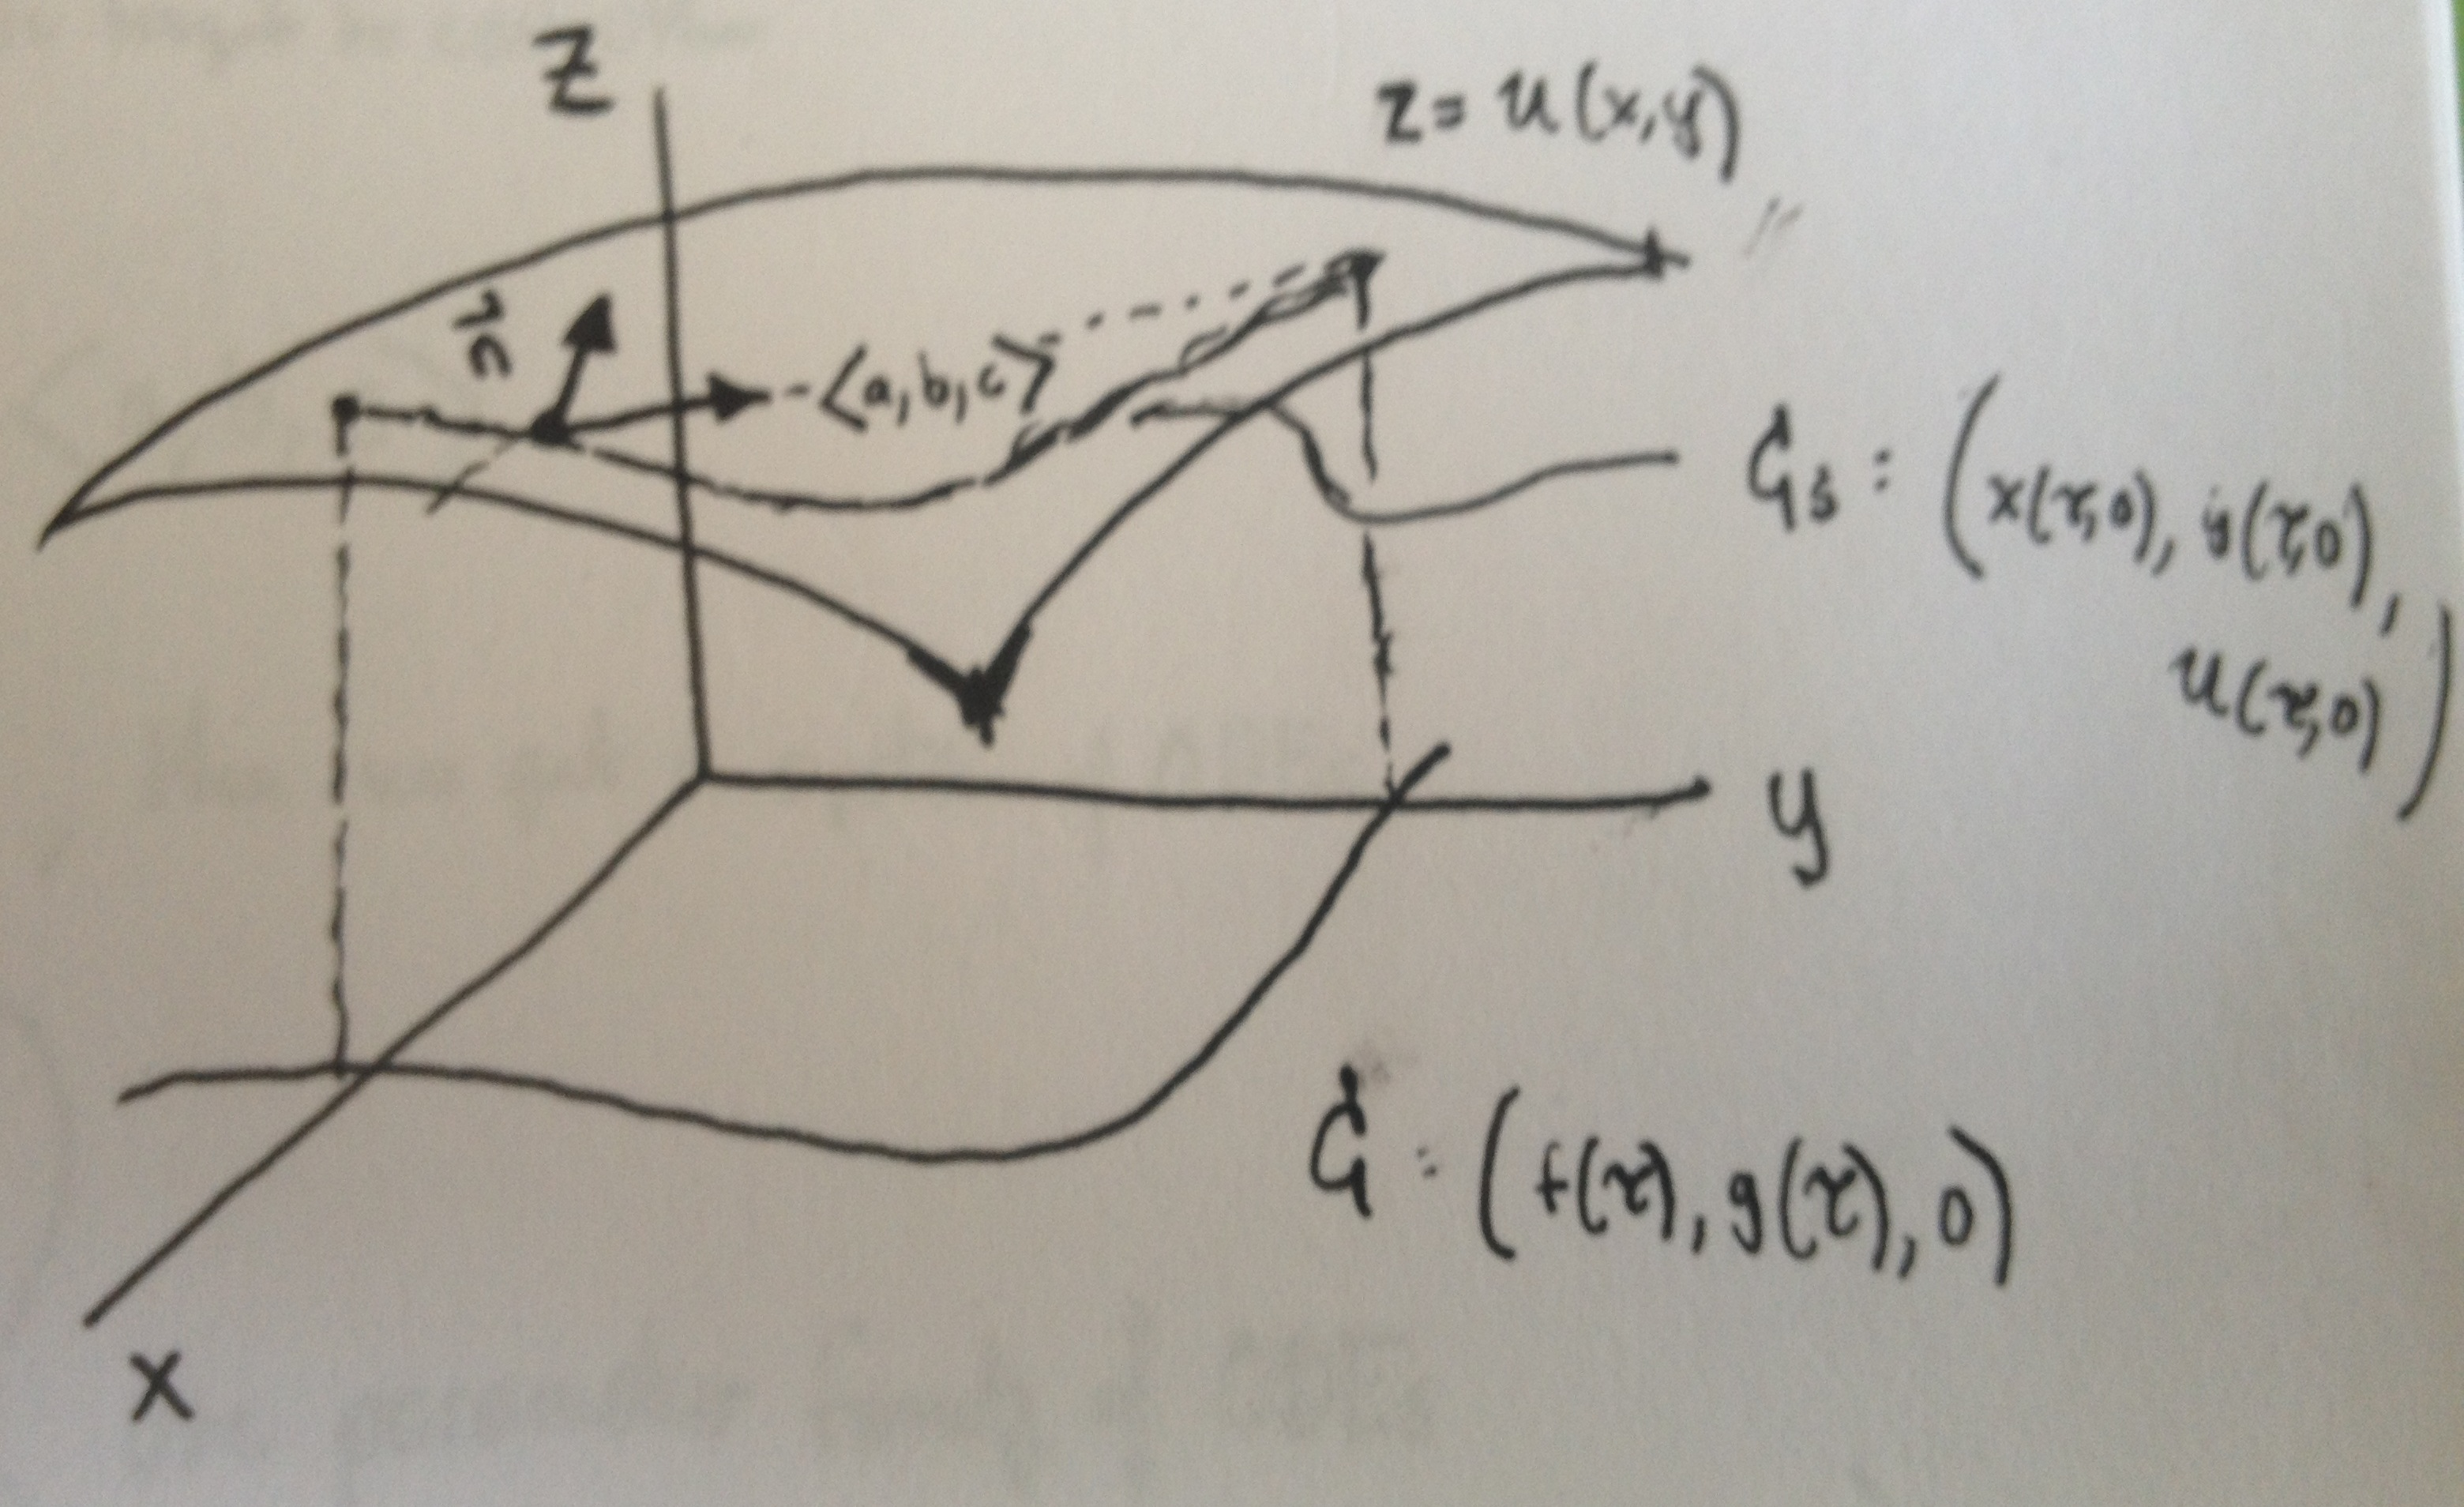
\includegraphics[width=3.0in]{moc_idea1.jpg}
\caption{General idea of the Cauchy problem's initial data.}
\label{moc_idea1}
\end{figure}

\item The solution is going to be a surface in $z=u(x,y)$ for the Cauchy problem which contains the initial data, $\mathscr{C}: (x(\tau,0), y(\tau,0), u(\tau,0)).$ This can be seen in Figure(\ref{moc_idea1}).\\

This surface can be thought of as a level curve of the function, $F(x,y,z) = u(x,y)-z=0,$\\

with corresponding normal vector, ${\bf{n}} = \nabla F = <u_x,u_y,-1>.$

Notice that the vector $<a,b,c>$ lies in the tangent plane of the solution surface at each point on it, e.g., $$<a,b,c>\cdot {\bf{n}} = <a,b,c>\cdot<u_x,u_y,-1> = au_x + bu_y - c = 0.$$

Following the vector $<a,b,c>$, it directs us along a curve on the solution surface. 
\begin{itemize}
\item[(i)] Such a curve passes through each point of the initial data curve, $\mathscr{C}_s$, given a one-parameter family of curves, with the parameter, $\tau$, specifying which one. 
\item[(ii)] Define $\tau$ so that it is constant along each curve, thus giving a one-parameter family of curves.  The curves are then the level curves of $\tau(x,y)=constant$.
\item[(iii)] Only $s$ varies along each curve, with $s=0$, corresponding to the points on the initial data curve, $\mathscr{C}_s$.

\begin{figure}[h!]
\centering
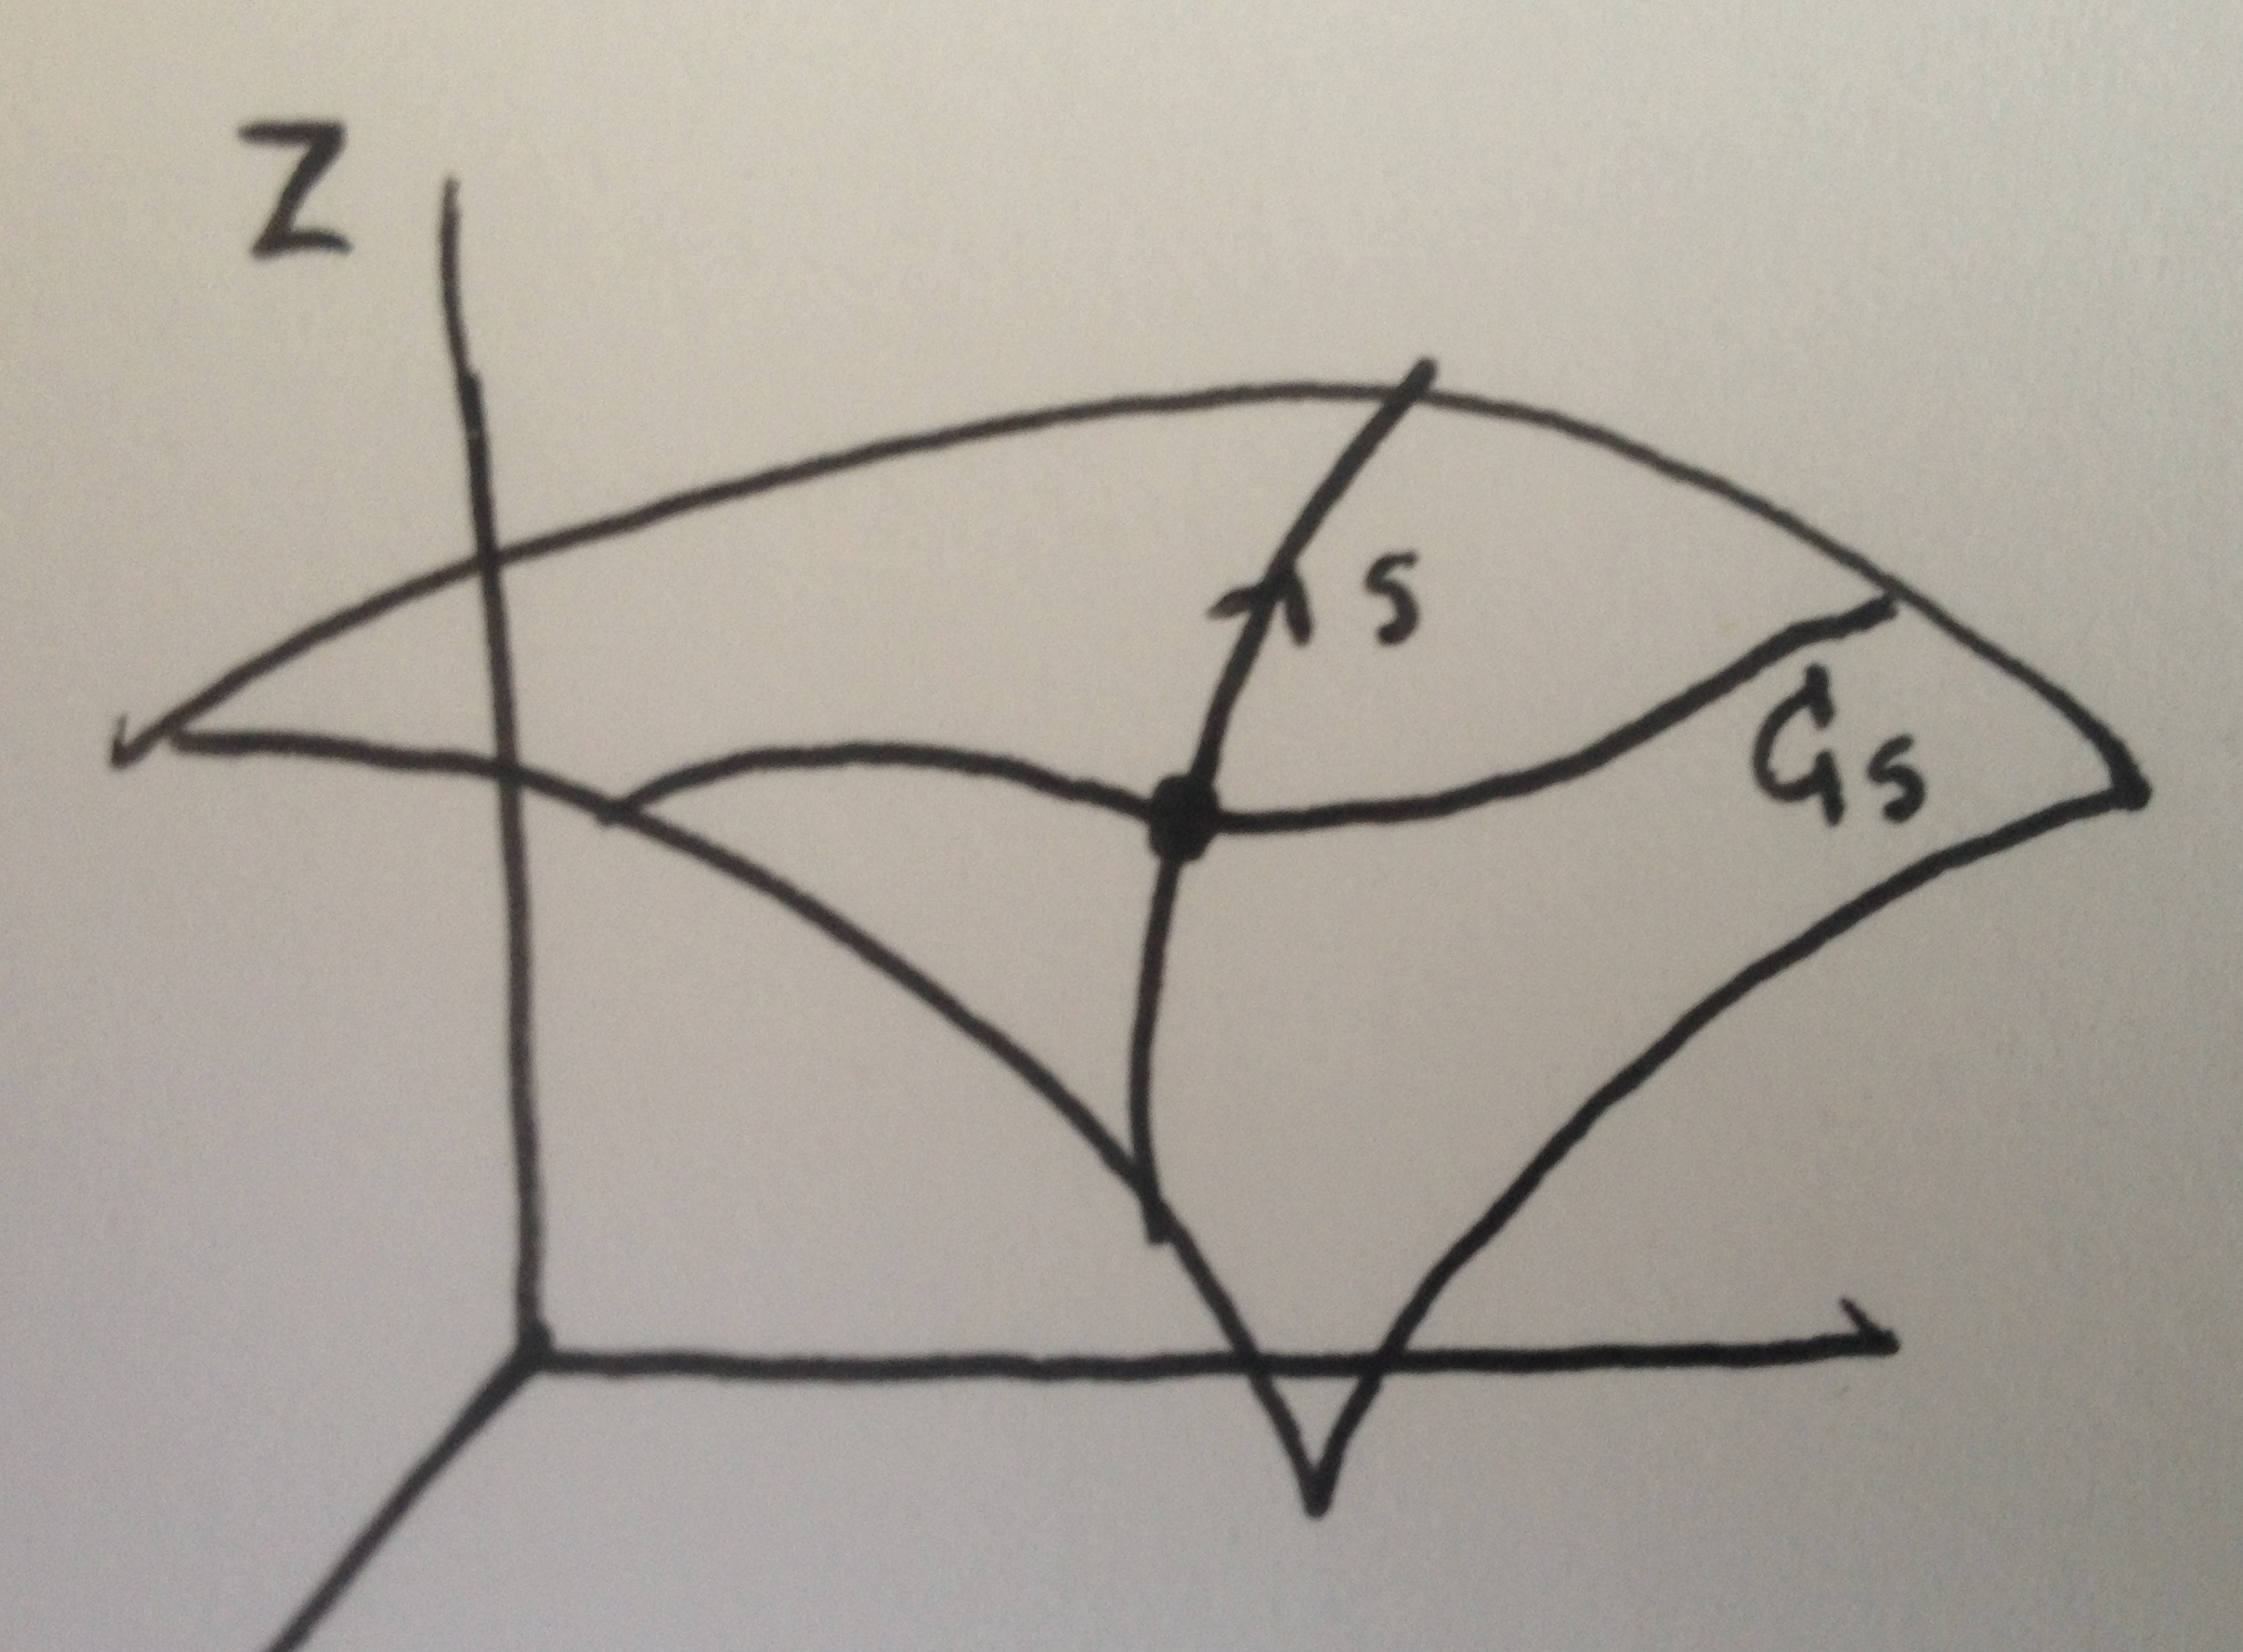
\includegraphics[width=3.0in]{moc_idea3.jpg}
\caption{Parameterized curve, with parameter $s$, going through initial data curve $\mathscr{C}_s$.}
\label{moc_idea3}
\end{figure}
\item[(iv)] For a fixed $\tau$, say $\tau=\tau_1$, the curve passing through the point $(x(\tau,0),y(\tau,0),u(\tau,0))$ on $\mathscr{C}_s$ can be considered as a parametric curve with parameter $s$. This idea is illustrated in Figure(\ref{mod_idea3}).
\item[(v)] A tangent vector to the parametric curve is: $\left< \frac{\partial x}{\partial s}, \frac{\partial y}{\partial s},  \frac{\partial u}{\partial s} \right>.$ 
\item[(vi)] The vector $<a,b,c>$ is also tangent to this curve!
\item[(vii)] Therefore $<a,b,c>$ and $\left< \frac{\partial x}{\partial s}, \frac{\partial y}{\partial s},  \frac{\partial u}{\partial s} \right>$ must be tangent to each other! E.g.,
$$\left< \frac{\partial x}{\partial s}, \frac{\partial y}{\partial s},  \frac{\partial u}{\partial s} \right> = k <a,b,c>,$$
where we can scale our parameter $s$ so such $k=1$ and we get the following system of ODEs
$$\left. \begin{array}{c}
\frac{\partial x}{\partial s} = a(x,y,u) \\
\frac{\partial y}{\partial s} = b(x,y,u) \\
\frac{\partial u}{\partial s} = c(x,y,u) \\
\end{array} \right\} \ \ \mbox{One parameter family of ODEs, called the \emph{characteristic equations} }.$$
Therefore we have
$$\frac{\partial u}{\partial s}  = \frac{\partial u}{\partial x} \frac{\partial x}{\partial s} + \frac{\partial u}{\partial y} \frac{\partial y}{\partial s} = a u_x + bu_y = c.$$

\item Finally, we have parameterized the initial data curve, $\mathscr{C}$, as 
\begin{align*}
x(\tau,0) &= f(\tau) \\
y(\tau,0) &= g(\tau) \\
u(\tau,0) &= u_0(\tau) \\
\end{align*}

The system of ODEs with these initial conditions yield a solution, 
\begin{align*}
x&=x(\tau,s) \\
y&=y(\tau,s) \\
u&=u(\tau,s) \\ 
\end{align*}
and upon inverting the transformation, if possible, i.e., solving for $\tau(x,y)$ and $s(x,y)$, we can arrive at our final solution, $$u(x,y) = u(\tau(x,y),s(x,y).$$
 
\end{itemize}

\end{enumerate}

%
% Mechanical Steps for Method of Characteristics!
%
\subsubsection{Mechanical Steps for the Method of Characteristics}

If the above description was not clear on the mechanistic approach, we will succinctly place the steps for the method of characteristics below. We again consider the Cauchy problem, $$a(x,y) u_x + b(x,y) u_y = c(x,y,u) \ \ \ \mbox{ with } \ \ \ u|_{\mathscr{C}} = u_0.$$

\begin{itemize}
\item[] {\bf{Step 1}}: Parameterize $\mathscr{C}$ in terms of $\tau$ and $s=0$,  $$\mathscr{C}: \left\{ \begin{array}{c} x=x(\tau,0) \\ y=y(\tau,0) \\ u=u(\tau,0) = u(x(\tau,0),y(\tau,0)) = u_0(\tau) \end{array} \right.$$
\item[] {\bf{Step 2}}: Solve the system of ODEs given by:
\begin{align*}
\frac{dx}{ds} &= a(x,y,u) \\
\frac{dy}{ds} &= b(x,y,u) \\
\frac{du}{ds}&= c(x,y,u) \\
\end{align*}
all subject to the initial conditions from Step 1. This then yields the following relation,
\begin{align*}
x&=x(\tau,s) \\
y&=y(\tau,s) \\
u&=u(\tau,s) \\
\end{align*}
\item[] {\bf{Step 3}}:  Solve for $s$ and $\tau$ in terms of $x$ and $y$, if possible*. Then $$u(x,y) = u(\tau(x,y),s(x,y)).$$ *Unfortunately, the coordinate transformations are not always invertible, or explicit in nature!

\end{itemize}


We will now present a few useful theorems regarding the method of characteristics. These all will be in the vein of the existence and uniqueness of solutions. 

\begin{theorem}
(\emph{Cauchy-Kowaleski Theorem}): Consider the Cauchy problem, $a(x,y,u) u_x + b(x,y,u) u_y - c(x,y,u)$ subject to a prescribed $u$ on a parametric curve, $\mathscr{C}: \left\{ \begin{array}{c} x = \bar{x}(\tau) \\ y=\bar{y}(\tau) \end{array} \right.,$ then we can let $u=u(\bar{x}(\tau),\bar{y}(\tau) )=u_0(\tau)$ for initial data. Suppose $a,b,c$ are continuously differentiable in a neighborhood of the initial data, i.e., the space curve $(\bar{x}(\tau), \bar{y}(\tau), u_0(\tau)).$ If 
$\left| \begin{array}{cc} a & b \\ X_\tau &Y_\tau \end{array}\right| \neq 0$ at all points on $\mathscr{C}$ (e.g., $\mathscr{C}$ is non-characteristic), then there exists a unique solution to the Cauchy problem in some neighborhood of the initial data curve, $\mathscr{C}.$
\end{theorem}

The following theorem can be used to identify when a Cauchy problem will have $\infty$-many solutions or no solution, based on the initial data.

\begin{theorem}
If $\left| \begin{array}{cc} a & b \\ X_\tau & Y_\tau \end{array}\right| = 0$ for all points on $\mathscr{C}$ (initial data curve itself is a characteristic), then the Cauchy problem has either $\infty-$many solutions or no-solution in a neighborhood of $\mathscr{C}.$
\end{theorem}

Throughout all of this analysis, we have employed use of the \emph{Implicit Function Theorem}, which tells us when we can invert a coordinate transformation. 
\begin{theorem}
(\emph{Implicit Function Theorem}) Consider $N$ equations with $N+M$ variables, $$F_k(x_1,x_2,\ldots,X_M,Y_1,\ldots,Y_N) = 0 \ \ \ \mbox{ for } \ \ \ k=1,2,\ldots,N,$$
or $${\bf{F}}({\bf{x}},{\bf{y}}) = 0.$$
We also assume each partial derivative of $F$is $C^1$ with respect to each $N+M$ variable. Furthermore we assume that the system of equations is satisfied at some point $P_0 = (x_1^0,\ldots,x_M^0,y_1^0,\ldots,y_N^0)$ with $$\left| \frac{\partial(F_1,\ldots,F_N)}{\partial(y_1,\ldots,y_N)} \right|_{P_0} \neq 0.$$
Then $\{y_k\}_{k=1}^{N}$ can be expressed as functions of $\{x_j\}_{j=1}^{M}$ in some neighborhood of $P_0$, i.e.,
\begin{align*}
y_1 = \phi_1(x_1,\ldots,x_M) \\
&\cdots \\
y_N = \phi_N(x_1,\ldots,x_M) \\
\end{align*}
or $${\bf{y}} = \vec{\phi}({\bf{x}}).$$
Moreover each $\{ \phi_k \}_{k=1}^{N}$ is $C^1$ with respect to each $\{x_j\}_{j=1}^{M}.$
\end{theorem}

The \emph{Implicit Function Theorem} in a nutshell, basically states that when we are given $\xi = \xi(x,y)$ and $\eta=\eta(x,y)$, we can write $x=x(\xi,\eta)$ and $y=y(\xi,eta)$ whenever $$\left| \begin{array}{cc} \xi_x & \xi_y \\ \eta_x & \eta_y \end{array} \right| \neq 0.$$

It is time to do an example! \emph{Let's boogey!}



%
% Method of Characteristics Example!
%
\subsubsection{Example: $x u_x - y u_y = 2xy^2$ with $u(x,1)=1+x^2$ on $0<x<1$}

Considering the PDE listed above. We will proceed with each of the mechanical steps we listed previously for solving a PDE using method of characteristics.

\begin{itemize}
\item[] {\bf{Step 1}}: Parameterize $\mathscr{C}$ with $\tau$ and $s=0$:
$$\mathscr{C}: \left. \begin{array}{c} x(\tau,0) = \tau \\ y(\tau,0) = 1 \end{array}\right\} \Rightarrow u(x(\tau,0),y(\tau,0))=u(\tau,1) = 1+\tau^2.$$

\item[] {\bf{Step 2}}: We setup the characteristics ODEs,
\begin{align*}
\frac{\partial x}{\partial s} &= x \\
\frac{\partial y}{\partial s} &= -y \\
\frac{\partial u}{\partial s} &= 2xy^2 = 2 \tau e^s e^{-2s} = 2\tau e^{-s}.
\end{align*}

Therefore solving the above system, we obtain
\begin{align*}
x &= Ke^{s}\Big|_{x(\tau,0)=\tau} \Rightarrow x=\tau e^s \\
y &= Ke^{s}\Big|_{y(\tau,0)=1} \Rightarrow y=e^{-s} \\
u(s) &= -2\tau e^{-s}+K\Big|_{u(\tau,0)=1+\tau^2} \Rightarrow u(\tau,s) = -2\tau e^{-s} + \tau^2 +2\tau + 1\\
\end{align*}

\item[] {\bf{Step 3}}: Inverting the transformations, we get 
\begin{align*}
x &= \tau e^s \Rightarrow \tau = xe^s = xy \\
y&= e^{-s} \Rightarrow s = -\ln(y),\ \ y>0 
\end{align*}

Hence we get our final solution as 
$$u(\tau,s) = -2\tau e^{-s} + \tau^2 +2\tau + 1 \Leftrightarrow  u(x,y) = -2xy^2 + 2xy + 1 + (xy)^2 = -2xy^2 + (xy+1)^2.$$

\end{itemize} $ $ \\ 

%
% General Method of Characteristics (for fully Nonlinear problem!)
%
\subsection{General Method of Characteristics for fully Nonlinear problems!}

In the above method of characteristics description, we have intentionally talked about the method of characteristics as used for \emph{quasi-linear} first-order PDEs. There is a more general version of the method of characteristics for fully nonlinear problems. We will describe the more general version now, but without much motivation. \\

The general method of characteristics in all its glory attempts to solve first-order PDEs of the form, $$F(x,y,u,u_x,u_y)=0,$$ with corresponding initial data $$\mathscr{C}: \left. \begin{array}{c} x=x(\tau) \\ y=y(\tau) \\ u(x(\tau),y(\tau)) = u(\tau) \end{array} \right\}.$$

First we use the following notation,
$$\left. \begin{array}{c}
p = u_x \\
q = u_y \\
\end{array} \right\} \Rightarrow \ \ \mbox{ standard notation}.$$

We will require that $u_x^2 + u_y^2 \neq 0,$ e.g., $p\neq 0$ when $q=0$ and vice-versa. We note that this mandates that the solution will not have any \emph{local} minima or maxima. Our governing PDE equation now takes the form, 

$$F(x,y,u,p,q) = 0.$$

Rolling through nonlinear method of characteristics rigmarole, which we do not expand upon here, we arrive at the following system of ODEs to solve,
\begin{align*}
\frac{dx}{ds} &= \frac{\partial F}{\partial p} \\
\frac{dy}{ds} &= \frac{\partial F}{\partial q} \\
\frac{du}{ds} & p\frac{\partial F}{\partial p} + q\frac{\partial F}{\partial q} \\
\frac{dp}{ds} &= -\left( \frac{\partial F}{\partial x} + p\frac{\partial F}{\partial u} \right) \\
\frac{dq}{ds} &= -\left( \frac{\partial F}{\partial y} + q\frac{\partial F}{\partial u} \right) \\
\end{align*}

with initial conditions $x(\tau,0)=x(\tau), y(\tau,0)=y(\tau), u(\tau,0)=u(\tau), p(\tau,0)=p(\tau), q(\tau,0)=q(\tau).$ For the initial conditions on $p(\tau)$ and $q(\tau)$, we use the conditions that

\begin{enumerate}
\item $F(x(\tau),y(\tau),u(\tau),p(\tau),q(\tau)) = 0$ \ \ \ (The differential equation is satisfied on the initial curve)
\item From $u_\tau = u_x x_\tau + u_y y_\tau$ on $\mathscr{C}$ we have that $u'(\tau) = p(\tau) x'(\tau) + q(\tau) y'(\tau).$
\end{enumerate}

Using those two bits of information we will be able to pick out the correct initial data for $p(\tau,0)$ and $q(\tau,0)$. We will leave you with just a few more notes on the general method of characteristics. 
\begin{enumerate}
\item Characteristics are still given by the level curves of $\tau(x,y)$.
\item If $F(x,y,u,p,q)$ is linear in $u_x$ and $u_y$, the above system reduces to the ``less-general" method of characteristics described previously
\item If $\left| \begin{array}{cc} x_\tau & x_s \\ y_tau & y_s \end{array}\right| = \left| \begin{array}{cc} x_\tau & F_p \\ y_tau & F_q \end{array}\right| = - \left| \begin{array}{cc} F_p & F_q \\ x_tau & y_\tau \end{array}\right| \neq 0$ on $\mathscr{C}$, then we are guaranteed a unique solution in some neighborhood of $\mathscr{C}.$
\end{enumerate}

Let's do an example for completeness!

%
% Nonlinear Method of Characteristics Example
%
\subsubsection{General Method of Characteristics Example: $u_x u_y = 1$ subject to $u(x,1) = 2\sqrt{x}$ for $x>0$}

First we write our first-order PDE in the form $$F(x,y,u,p,q) = u_x u_y -1 = pq -1,$$ with $p=u_x$ and $q=u_y$. We also note that $F_x=F_y=F_u=0,$ as well that $q = F_p$ and $p=F_q$. We then have the following system of ODEs to solve,
\begin{align*}
\frac{dx}{ds} &= F_p = q \\
\frac{dy}{ds} &= F_q = p \\
\frac{du}{ds} &= pF_p + qF_q = 2pq \\
\frac{dp}{ds} &= 0\\
\frac{dq}{ds} &= 0\\
\end{align*}
with initial conditions $x(\tau,0)=\tau, y(\tau,0)=1, u(\tau,0)=2\tau^{1/2}.$ Recall that on $\mathscr{C}$ the initial data is satisfied, hence we have 
\begin{itemize}
\item[(i)] $pq-1 = 0\Rightarrow p = \frac{1}{q} $ 
\item[(ii)] $u'(\tau) = pX'(\tau) + qY'(tau) \Rightarrow \tau^{1/2} = p(\tau,0)(1) + q(\tau,0)(0) = p$
\end{itemize}
on $\mathscr{C}$. Solving this system, we find that $$p(\tau,0) = \tau^{-1/2} \ \ \ \mbox{and} \ \ \ q(\tau,0)=\tau^{1/2}.$$

Now we have all the initial data we require and can proceed to solving the above system. Upon solving all these ODEs we find
\begin{align*}
\frac{dp}{ds} &= 0 \Rightarrow p(\tau,s) = C\Big|_{p(\tau,0)=\tau^{-1/2}} \Rightarrow p(\tau,s) = \tau^{-1/2} \\
\frac{dq}{ds} &= 0 \Rightarrow q(\tau,s) = C\Big|_{q(\tau,0)=\tau^{1/2}} \Rightarrow q(\tau,s) = \tau^{1/2} \\
\frac{dx}{ds} &= q \Rightarrow x(\tau,s) = \tau^{1/2}s + A(\tau)\Big|_{x(\tau,0)=\tau} \Rightarrow A(\tau) = \tau  \\
\frac{dy}{ds} &= p \Rightarrow y(\tau,s) = \tau^{-1/2}s + B(\tau)\Big|_{y(\tau,0)=1} \Rightarrow B(\tau) = 1  \\
\frac{du}{ds} &= 2pq \Rightarrow  u(\tau,s) = 2s + C(\tau)\Big|_{u(\tau,0)=2\tau^{1/2}} \Rightarrow C(\tau) = 2\tau^{1/2} \\
\end{align*}

and hence get
\begin{align*}
x(\tau,s) &= \tau^{1/2} s + \tau \\
y(\tau,s) &= \tau^{-1/2}s + 1\\
u(\tau,s) &= 2s+2\tau^{1/2}.\\
\end{align*}

Now we must try to transform back into $(x,y)$ coordinates from $(\tau,s)$. From the above relations, we see we can write 
$$\tau y = \tau^{1/2}+\tau = x,$$

and thereby $$x -\tau y = 0 \Rightarrow \tau = \frac{x}{y}.$$

Hence we find $$s = \left(\frac{x}{y}\right)^{1/2}(y-1),$$

and obtain as our final solution $$u(x,y) = 2\left(\frac{x}{y}\right)^{1/2}(y-1) + 2\left( \frac{x}{y} \right)^{1/2} = 2\sqrt{xy}.$$

We also state that the characteristics for the above problem are $\tau = \frac{x}{y} = constant.$

%%%%%%%%%%%%%%%%%%%%%%%%%%%%%%%%%%%%%
%
% SEPARATION OF VARIABLES
%
%%%%%%%%%%%%%%%%%%%%%%%%%%%%%%%%%%%%%

\subsection{Separation of Variables: For $2^{nd}$ order linear PDE (finite domains)}

In this section we will discuss a powerful method for finding solutions to linear PDE on finite domains. This is not the end-all, be-all technique for solving linear PDEs, but is very useful in areas from mechanics, electromagnetism, quantum mechanics, to economics. \\

We will show illustrate this method through an example.

\begin{itemize}
\item[] {\bf{Example}}: Heat Equation in $1d$ on a finite domain

Consider the following first-order linear constant coefficient, homogeneous PDE, $$u_t = \kappa u_{xx},$$ with associated boundary conditions $u(0,t)=u(1,t)=0,$ and initial value $u_0(x)=u(x,0) = f(x)$. Hence we consider the domain $x\in[0,1]$ and $t>0$. \\

We begin by assuming a solution of the form $$u(x,t)=X(x)T(t),$$ that is, $u(x,t)$ can be written as a product of two functions, one function with functional dependance only on $x$, and the other with functional dependence only on $t$. Performing that substitution we see 

$$u_t = \kappa u_{xx} \Rightarrow \frac{T'(t)}{T(t)} = \kappa \frac{X''(x)}{X(x)}.$$

From the above we see that since each side of the equation depends only on one independent variable, yet are equal for any values, that the quantity above must be equal to a constant, say $-\alpha^2.$ Hence we have 

$$\frac{T'(t)}{\kappa T(t)} =  \frac{X''(x)}{X(x)} = -\alpha^2.$$

We now have an eigenvalue in our problem...err...one more degree of freedom to work with! Before we get to that, we note that the boundary conditions are still to be obeyed, and are enforced via the $X(x)$ function, i.e., $ X(0)=X(1)=0.$ Now let's solve the above problem!\\

\begin{itemize}

%Solving T'(t) Equation
\item[] {\bf{Solving: $T'(t) = - \kappa\alpha^2 T(t)$}} \\ \\
We can solve this ODE simply by noticing its beautiful separable form, 
$$\frac{dT}{T} = -\kappa\alpha^2 dt,$$
and hence by simple integration obtain
$$T(t) = c_0 e^{-\kappa\alpha^2 t}.$$

We note that we did not get any information about the eigenvalue from solving this, nor can be use the initial value yet, since there is much spatial information to be learned! \\

\item[] {\bf{Solving: $X''(x) + \alpha^2 X(x) = 0.$}} \\ \\
In solving this equation we have to look at three cases, that is when $\alpha=0$, $\alpha^2 < 0$, and $\alpha^2>0.$\\
\begin{enumerate}

\item ${\bf{\alpha=0}}$: $$X'' = 0$$
and hence we have $$X(x) = cx+d.$$
Using the boundary conditions we see that $$X(0)=X(1)=0 \Rightarrow c=d=0,$$
and hence we only have the trivial solution.\\

\item ${\bf{\alpha^2 <0}}:$ $$X'' - \alpha^2 X = 0$$
Solving this we get in general that $$X(x) = c\sinh(\alpha x) + d\cosh(\alpha x).$$
Using the boundary conditions we see that 
\begin{align*}
X(0) &= d = 0\\
X(1) &= c\sinh(\alpha) = 0 \Rightarrow c = 0\\
\end{align*}
since we've assumed that $\alpha\neq0$ in this case. Hence we again only have the trivial solution present.\\

\item ${\bf{\alpha^2 > 0}}$: $$X'' + \alpha^2 X = 0$$

Solving the above ODE, we get $$X(x) = c\sin(\alpha x) + d\cos(\alpha x).$$

Now using the boundary conditions we find
\begin{align*}
X(0) &= d = 0 \\
X(1) &= c\sin(\alpha) = 0 \Rightarrow \alpha = n\pi \\
\end{align*}

where $n\in\mathbb{N}$. Therefore we find that our eigenvalue, $\lambda = \alpha^2 = n^2\pi^2.$ 

\end{enumerate}

\end{itemize}

Now we have both our solutions, $$u(x,t) = X(x)T(t) = c \sin(n\pi x) e^{-\kappa n^2 \pi^2 t};$$

however, we see that any positive integer value of $n$ gives us a different eigenvalue. It makes sense in fact we can use superposition to sum all of these possible solutions, each corresponding to a different eigenvalue, e.g.,

$$u(x,t) = \sum_{n=1}^{\infty} c_n  \sin(n\pi x) e^{-\kappa n^2 \pi^2 t}.$$

Note that we still have an infinite amount of coefficients $\{ c_j \}$ to find! Where, oh where, will we be able to find these? Welp, we haven't used the initial value for anything, yet. Let's start there!\\

Using the initial value, $u(x,0)=u_0(x) = f(x)$, we see that we have $$f(x) = \sum_{n=1}^{\infty} c_n \sin(n\pi x).$$ The above is simply a Fourier Series for $f(x)$! We can use the tricks and tools of the trade, i.e., orthogonality and completeness of the Fourier basis, to find $\{ c_n\}$.\\

Using Fourier Series, we note that we get

$$c_n = \frac{2}{L} \int_0^1 f(x) \sin(n\pi x) dx.$$

Therefore the final solution to our heat equation problem is $$u(x,t) =\frac{2}{L}  \sum_{n=1}^{\infty} \left[ \int_0^1 f(\tilde{x}) \sin(n\pi \tilde{x}) d\tilde{x} \right] \sin(n\pi x) \ e^{-\kappa n^2 \pi^2 t}.$$

$ $\\

%
% NON-HOMOGENOUS EXAMPLE
%
\item[] {\bf{Non-homogeneous Heat Equation}}

Consider the following first-order linear constant coefficient, non-homogeneous PDE, $$u_t = R + k u_{xx},$$ with associated boundary conditions, one of which is non-homogeneous, e.g., $u(0,t)=0$ and $u(1,t)=u_0$ for $t>0$, and initial value $u_0(x)=u(x,0) = f(x)$ for $0<x<1$. Hence we consider the domain $x\in[0,1]$ and $t>0$. \\

For problems of this type, we will begin by making a change of variables of the dependent variable, 
\begin{equation}
\label{nonhomo_change} u(x,t) = \psi(x,t) + \xi(x)
\end{equation}

Recal the boundary conditions in our new change of variables, 
\begin{align*}
u(0,t) &= \psi(0,t) + \xi(0) = 0 \\
u(1,t) &= \psi(1,t) + \xi(1) = 0 \\
\end{align*}

We will be able to put the non-homogeneous term all on the $\xi(x)$ function, provided we have $$\xi(0) = 0 \ \ \ \mbox{ and } \ \ \ \xi(1) = u_0.$$ In this case we then have translated homogeneous boundary conditions to $\psi(x,t)$ on $[0,1]$. We note that since $\xi(x)$ has no $t$ dependence, the initial conditions gets placed onto $\psi(x,t)$, i.e., $$u(x,0) = f(x) =  \psi(x,0) + \xi(x) \Rightarrow \psi(x,0) = f(x) - \xi(x).$$

Differentiating (\ref{nonhomo_change}) accordingly, we have
$$\frac{\partial^2 u}{\partial x^2} = \frac{\partial^2 \psi}{\partial x^2} + \xi''(x) \ \ \ \mbox{ and } \ \ \ \ \frac{\partial u}{\partial t} = \frac{\partial \psi}{\partial t}.$$

Therefore our model PDE becomes
$$k\frac{\partial^2 \psi}{\partial x^2} + k\xi'' + R = \frac{\partial\psi}{\partial t}.$$

The above equation will reduce to a homogeneous equation if we make the assumption that $$k\xi'' + R = 0.$$

Solving this (by two simple integration) gives $$\xi(x) = -\frac{R}{2k}x^2 + c_1 x + c_2.$$

Now making $\xi(x)$ obey the boundary conditions we set above gives
$$c_1 = \frac{R}{2k}+u_0 \ \ \ \ \mbox{ and } \ \ \ \ \ c_2 = 0.$$ 

Hence we find $$\xi(x) = -\frac{R}{2k}x^2 + \left[ \frac{R}{2k}+u_0\right]x.$$

Once we have $\xi(x)$, we can now set out to solve our homogeneous PDE given above, e.g., $$\psi_t  = k \psi_{xx},$$ with $\psi(0,t)=\psi(1,t) = 0$ for $t>0$ and $\psi(x,0) = f(x) - \xi(x).$ \\

It is clear that finding the solution to this PDE is identical to solving the homogeneous heat equation we previously have, but with differing initial condition. Rolling through the same separation of variables rigmarole, we find that 

$$\psi(x,t) = \sum_{n=1}^{\infty} c_n e^{-k n^2 \pi^2 t} \sin(n\pi x),$$

where we known the $\{c_j\}'s$ are given by orthogonality of the Fourier basis, 

$$c_n =  \frac{  \int_{0}^{1} \left[ f(x) + \xi(x) \right] \sin(n\pi x) dx }{\int_{0}^{1} \sin^2(n\pi x) dx } = 2 \int_{0}^{1} \left[ f(x) + \frac{R}{2k}x^2 - \left(\frac{R}{2k}+u_0\right) x \right] \sin(n\pi x) dx.$$

Therefore the solution to our original non-homogeneous PDE is given by
\begin{align*}
u(x,t) &= \psi(x,t) + \xi(x)\\ 
&=\sum_{n=1}^{\infty} \left[ \int_{0}^{1} \left[ f(\tilde{x}) + \frac{R}{2k}\tilde{x}^2 - \left(\frac{R}{2k}+u_0\right) \tilde{x} \right] \sin(n\pi \tilde{x}) d\tilde{x} \right] e^{-kn^2  \pi^2 t} \sin(n\pi x)   -  \frac{R}{2k}x^2 + \left[ \frac{R}{2k}+u_0\right]x.\\
\end{align*}

We note that the above solution is composed of two pieces, $\psi(x,t)$ and $\xi(x).$ We call $\xi(x)$ the \emph{steady-state} solution since we note that as $t\rightarrow\infty, \psi(x,t)\rightarrow 0$. We call $\psi(x,t)$ the \emph{transient} solution.

%
% Notes of Separation of Variables
%
\item[] {\bf{A few more notes on separation of variables}}: \\ \\

We will just say a few brief things about this method.
\begin{enumerate}
\item This methodology be used only for linear PDEs on finite domains
\item Such PDEs do not have to have constant coefficients; however, as long as the equation is separable and the resulting systems of ODEs leads to be of the \emph{Sturm-Liouville} flavor, you will be able to use this method
\item The example above easily goes through the mechanics and solutions to the wave equation and Laplace's Equation can be done analogously.
\item This methodology will work for higher order heat equations, wave equations, Laplace's equations, e.g., situations with more than two independent variables.
\item The change of variables, $u(x,t) = \psi(x,t) + \xi(x)$, will work for non-homogeneous problems involving Laplace's equation or the wave equation, as well.
\end{enumerate}


\end{itemize} %ENDS HEAT EQUATION EXAMPLE


%%%%%%%%%%%%%%%%%%%%%%%%%%%%%%%%%%%
%
% INTEGRAL TRANSFORMs for PDE
%
%%%%%%%%%%%%%%%%%%%%%%%%%%%%%%%%%%%

\subsection{Integral Transforms: Linear PDEs on $\mathbb{R}\ (or \mathbb{R}^n)$}

In this section we will show how to use the Fourier Transform, Laplace Transform, and alike methods for solving some linear PDEs. In general for linear PDEs on $\mathbb{R}$, we will use the \emph{Fourier Transform}, while for variables defined on $[0,\infty)$ we will use the \emph{Laplace Transform}. We will begin with a brief overview of the \emph{Fourier Transform}

%
% FOURIER TRANSFORM
%
\subsubsection{The Fourier Transform}

We begin with the definition of the Fourier Transform,
\begin{equation}
\label{Fourier_Transform} \mathscr{F}\{f(x)\}(k) = F(k) =  \int_{-\infty}^{\infty} f(x) e^{-ikx} dx.
\end{equation}

We note that not every function $f(x)$ will have a Fourier Transform; however, a sufficient condition for a function to have one (i.e., the above integral converges) is that $f(x)$ is square-integrable, e.g., $$||f(x)||^2 = \int_{\mathbb{R}} |f(x)|^2 dx = \mbox{ a constant}.$$ 

If $f(x)$ is also continuous as well, then the Inverse Fourier Transform should exist, and we have the inversion formula 
\begin{equation}
\label{Inverse_Fourier_Transform} f(x) =\frac{1}{2\pi} \mathscr{F}^{-1}\{ F(k) \}(x) = \int_{\mathbb{R}} F(k) e^{ikx} dk.
\end{equation}

We will now discuss a few properties of the Fourier Transform.

\begin{enumerate}

%Linearity
\item {\bf{Linearity}}: \\ \\

Like the Laplace Transform, linearity holds in the Fourier Transform. If it didn't, it probably wouldn't be worth a second glance, after-all.
$$\mathscr{F}\{ c_1 f_1(x) + c_2 f_2(x) \} = c_1 \mathscr{F}\{f_1(x)\} + c_2\mathscr{F}\{f_2(x) \} = c_1F_1(k) + c_2F_2(k),$$

where $\{c_1,c_2\}\in\mathbb{C}.$ 

%Translation
\item {\bf{Translations}}: \\ \\

We also have the following translational property,
\begin{align*}
\mathscr{F}\{ f(x-a)\} &= \int_{\mathbb{R}} f(x-a) e^{-ikx} dx \\
&= \int_{\mathbb{R}} f(u) e^{-ik(u+a)} du \\
&= e^{-ika} \int_{\mathbb{R}} f(u) e^{-iku} du \\
&= e^{-ika} F(k)\\
\end{align*}

Hence we have $$\mathscr{F}\{ f(x-a)\} =e^{-ika} F(k).$$

%SCALING
\item {\bf{Scaling}}: \\ \\
The following scaling property also holds
$$\mathscr{F}\{ f(cx) \} = \frac{ F\left( \frac{k}{c} \right)}{|c|}.$$

%CONVOLUTION
\item {\bf{Convolution}}: \\ \\ 

The Fourier Transform of a convolution of two functions, $f_1(x)$ and $f_2(x)$, has an elegant (and convenient!) form,

$$\mathscr{F}\{ f_1(x)\ast f_2(x) \} = F_1(K) F_2(k).$$

%MODULATION
\item {\bf{Modulation}}: \\ \\

The Fourier Transform of a modulation (product) of functions is given by

$$\mathscr{F}\{ f_1(x)f_2(x)  \} = F_1(x) \ast F_2(x).$$

%PARSEVAL'S THEOREM
\item {\bf{Parseval's Theorem}}: \\ \\

$$\int_{\mathbb{R}} | f(x) |^2 dx = \int_{\mathbb{R}} | F(k) |^2 dk,$$ or equivalently

$$||F(k)||^2 = \frac{1}{2\pi} ||f(x)||^2.$$

This identity becomes especially useful when doing stability analysis of numerical methods involving finite differencing for the solutions of PDEs.

%Duality
\item {\bf{Duality}}: \\ \\

Suppose $f(x)$ has Fourier Transform $F(k)$. Then we immediately know the Fourier Transform of the function $F(x)$! This is known as the duality property of the Fourier Transform, as seen below

$$\mathscr{F}\{ F(x) \} = 2\pi f(-k).$$

%Derivatives!
\item {\bf{Derivatives!}}:\\ \\

When we take the Fourier Transform of a derivative, we will simply use our good friend, integration by parts, to help us out. Knowing that our function is square-integrable is what will allow us to drop terms. Let's check it out

\begin{align*}
\mathscr{F}\left\{\frac{df}{dx} \right\} &= int_{\mathbb{R}} \frac{df}{dx} e^{-ikx} dx \\
&= f(x)  e^{-ikx} \Big|_{\mathbb{R}} +  \int (-ik) f(x) e^{-ikx} dx \\
&= (-ik) \int_{\mathbb{R}} f(x) e^{-ikx} dx \\
&= (-ik) F(k)
\end{align*}

Therefore we find that $$\mathscr{F}\left\{\frac{df}{dx} \right\}  = (-ik) F(k).$$

We can continue analogously for higher order derivatives, and by induction, we get the following relation

$$\mathscr{F}\left\{ \frac{d^n f}{dx^n}  \right\} = (-ik)^n F(k).$$

%
% Derivative of FT of Non-Transformed Variable
%
\item {\bf{Derivatives with respect to non-transformed variables}}:\\ \\

Consider taking the Fourier Transform \emph{with respect to} $x$ of $\frac{\partial u}{\partial t}.$ We will see since $t$ is a dummy-type variable and our integration does not depend on it, it makes sense we will be able to pull the derivative operator with respect to $t$ out of the integral. Let's check it out rigorously,

\begin{align*}
\mathscr{F}\left\{ \frac{\partial u}{\partial t} \right\} &= \int_{\mathbb{R}} u_t(x,t) e^{-ikx} dx \\
&= \int_{\mathbb{R}} \frac{ u(x,t+\Delta t) - u(x,t) }{\Delta t} e^{-ikx} dx \\
&= \lim_{\Delta t\rightarrow 0} \frac{1}{\Delta t} \left[ \int_{\mathbb{R}} u(x,t+\Delta t) e^{-ikx} dx - \int_{\mathbb{R}} u(x,t) e^{-ikx} dx  \right] \\
&= \lim_{\Delta t\rightarrow 0} \frac{1}{\Delta t} \left[ U(k,t+\Delta t) - U(k,t) \right] \\
&= \frac{\partial}{\partial t} U(k,t)\\
\end{align*}

Naturally this result holds for higher order derivatives, i.e.,
$$\mathscr{F}\left\{\frac{\partial^n u}{\partial t^n}  \right\} = \frac{\partial}{\partial t^n} U(k,t).$$
\end{enumerate}

Now let's proceed to solve a PDE using Fourier Transform! 


%
% USING FT TO SOLVE WAVE EQUATION
%
\subsection{Fourier Transform to Solve a PDE}

Consider the following hyperbolic equation, e.g., in this case the \emph{wave equation},
$$u_{tt} = c^2 u_{xx},$$ with $u\rightarrow0$ as $|x|\rightarrow \infty$ and for $t>0$. We begin by taking the Fourier Transform of both sides of this equation, 

$$\int_{\mathbb{R}} u_{tt} e^{-ikx} dx = \int_{\mathbb{R}} c^2 u_{xx} dx.$$

From properties of the Fourier Transform we saw in the previous section, we see that this gives us 

$$\frac{\partial^2 }{\partial t^2} U(k,t) = c^2 (-ik)^2 U(k,t) = -c^2k^2 U(k,t)$$

Hence taking the Fourier Transform has transformed our PDE into an ODE. We now just consider $k$ as some fixed parameter, and see our problem is reduced to a constant coefficient ,homogeneous linear ODE. We can easily solve this ODE using familiar methods from basic ODE theory. Let $$U(k,t) = e^{\alpha t},$$

and upon substituting we see we get the solution

$$U(k,t) = C_1(k)e^{-ickt} + C_2(k) e^{ickt},$$

where $C_1(k)$ and $C_2(k)$ are functions strictly of $k$ and will be able to be found via initial conditions. We note that when $k=0$, the ODE becomes singular and we instead have to solve $U_{tt} = 0$, which leads to the trivial solution when mandating that the solution remain physical. \\

Now to recover the solution we care about in physical space, i.e., $u(x,t)$, we need to use the Inverse Fourier Transform to transform back appropriately. Doing this we find
\begin{align*}
\mathscr{F}^{-1}\{ U(k,t)  \} &= \frac{1}{2\pi} \int_{\mathbb{R}} U(k,t) e^{-ikx} dk\\
&= \frac{1}{2\pi} \int_{\mathbb{R}} \left[ C_1(k) e^{-ickt} + C_2(k) e^{ickt} \right] e^{ikx} dk\\
&= \frac{1}{2\pi} \left[ \int_{\mathbb{R}} C_1(k) e^{ik(x-ct)} dk + \int_{\mathbb{R}} C_2(k) e^{ik(x+ct)} dk  \right] \\
&= c_1(x-ct) + c_2(x+ct) 
\end{align*}

where $C_1(k,t) = \int_{\mathbb{R}} c_1(x,t) e^{-ikx} dx$ and $C_2(k,t) = \int_{\mathbb{R}} c_2(x,t) e^{-ikx} dx$ and hence their Inverse Fourier Transforms are used above. We note that this solution is called the \emph{D'Alembert} solution, which describes wave phenomena, where one wave packet moves to the right, $c_1(x-ct)$, and one wave packet moves to the left, $c_2(x+ct).$


%
% USING LAPLACE TRANSFORM TO SOLVE WAVE EQUATION
%
\subsection{Laplace Transform to Solve a PDE}

Consider the following wave equation, $$u_{tt}=c^2 u_{xx},$$
with boundary conditions $u(0,t)=u(1,t) = 0$ for $t>0$, and initial values $u(x,0)=0$ and $u_t(x,0) = \sin(\pi x)$ on $0<x<1$. We note that the spatial domain is finite, making us consider another method besides Fourier Transforms. We could, of course, notice the equation is separable, and use separation of variables, but we already had our fun with those, and yurn to use integral transforms! \\

Since the variable $t$ is defined for $t\in[0,\infty),$ we can use Laplace Transforms to transform the equation in this variable. Taking the Laplace Transform of both sides of the equation gives

\begin{align*}
\mathscr{L}\left\{ \frac{\partial^2 u}{\partial t^2} \right\} &= \mathscr{L}\left\{ c^2 \frac{\partial^2 u}{\partial x^2} \right\} \\
\int_{0}^\infty u_{tt} e^{-st} dt &= \int_{0}^\infty c^2 u_{xx} e^{-st} dt \\
s^2 U(x,s) - s u(x,0) - u_t(x,0) &= c^2 \frac{ d^2 U}{dx^2} 
\end{align*}

and hence we have the following ODE to solve

$$U_xx - s^2 U = s u(x,0) + u_t(x,0) = \sin(\pi x),$$

by substituting our initial data. However, before we go further we recognize that the boundary conditions are functions of $t$ and hence themselves must be transformed as well,
\begin{align*}
\mathscr{L}\{ u(0,t)  \} &=  \mathscr{L}\{ 0 \} = 0 = U(0,t) \\
\mathscr{L}\{ u(1,t)  \} &=  \mathscr{L}\{ 0 \} = 0 = U(1,t).
\end{align*}

Now we have the appropriate boundary conditions to use when solve the ODE in the transformed space. Proceeding with the solution, we first solve the homogeneous problem, i.e., $U_xx - s^2 U = 0$, to get the complementary solution and find $$U_C(x,s) = c_1 \cosh(sx) + c_2 \sinh(sx),$$

since $s>0$ in the Laplace Transform. However, using the boundary conditions, we find that $c_1 = c_2 = 0.$ Onwards to solve for the particular solution, we can use the method of undetermined coefficients (or variation of parameters if you're really that bored), starting with an initial guess for the particular solution as $$U_P(x,s) = A \cos(\pi x) + B\sin(\pi x).$$

Substituting this into the ODE, we find that $A=0$ and $B=\frac{1}{s^2+\pi^2}.$ Therefore our solution is:

$$U(x,s) = U_C(x,s) + U_P(x,s) = \frac{1}{s^2+\pi^2} \sin(\pi x).$$

Now we must transform back into physical space, 
\begin{align*}
u(x,t) &= \mathscr{L}^{-1}\left\{ U(x,s)  \right\} \\
& =  \mathscr{L}^{-1}\left\{  \frac{1}{s^2+\pi^2} \sin(\pi x) \right\} \\
& = \frac{1}{\pi}  \mathscr{L}^{-1}\left\{  \frac{\pi}{s^2+\pi^2} \sin(\pi x) \right\} \\
&= \frac{1}{\pi} \sin(\pi x) \sin(\pi t).
\end{align*}




%%%%%%%%%%%%%%%%%%%%%%%%%%%%%%%%
%
% SIMILARITY SOLUTIONS
%
%%%%%%%%%%%%%%%%%%%%%%%%%%%%%%%%

\subsection{Similarity Solutions!}

Similar transformations can help give a lot of information about certain PDEs; however, we can also use them to cook up solutions when some of (or all) of the independent variables appear through certain groupings, rather than independently. Consider the following example involving the 2D heat equation.

\begin{enumerate}
\item {\bf{2D Heat Equation}} \\ \\
For example, if we consider the heat equation $$u_t = k(u_{xx} + u_{yy},$$ we can search for solutions that depend on $x$ and $y$ through the grouping, $$r(x,y) = \sqrt{x^2+y^2}, $$ e.g.,

$$u(x,y,t) \rightarrow u(r(x,y),t) = u(r,t),$$ and $$u_x = u_r r_x \Rightarrow u_{xx} = u_{rr} r_x^2 + u_r r_{xx} = u_{rr}\frac{x^2}{r^2} + u_r \frac{y^2}{r^3},$$
and analogously for $u_{yy}$ we get, $$u_{yy} = u_{rr}\frac{y^2}{r^2} + u_r \frac{x^2}{r^3},$$
and hence $$u_{xx}+u_{yy} = u_{rr}+\frac{1}{r} u_r.$$ Doing these substitutions leads to the radially symmetric heat equation, $$u_t = k\left[ u_{rr} + \frac{1}{r} u_r\right].$$

\item {\bf{1D Wave Equation}} \\ \\
Consider $$u_t + au_x = 0.$$ We will search for solutions of the form $u=u(\xi(x,t))$ where $\xi(x,t)=x-at.$ Performing the necessary derivatives, we get
$$u_t = u_\xi xi_t = -a u_\xi \ \ \ \mbox{ and } \ \ \ u_x = u_\xi \xi_x = u_\xi.$$ Therefore substituting these into the wave equation above we find
\begin{align*}
u_t + au_x &= 0 \\ 
(-au_\xi ) + a(u_\xi) &= 0\\
0&= 0 \Rightarrow \ \ \mbox{all differentiable functions of } \xi \mbox{ satisfy the PDE}.\\
\end{align*}

Therefore we find our solutions take the form $$u(x,t) = f(x-at).$$

We now make the claim that no solutions are lost by this similarity transformation. To see this we will find the solution using this idea of similarity transformation! We will make the full coordinate transformation, 
$$\xi = x-at \ \ \ \mbox{ and } \ \ \ \eta = \eta(x,t).$$
Recall from the Implicit Function Theorem if $$\left| \begin{array}{cc} \xi_x & \xi_t \\ \eta_x & \eta_t \end{array} \right| = \left| \begin{array}{cc} 1 & -a \\ \eta_x & \eta_t \end{array} \right| = \eta_t - a\eta_x \neq 0,$$ then we have an invertible transformation. We just need $\eta(x,t)$ to satisfy the above.

Performing the necessary derivatives we find
\begin{align*}
u_t &= u_\xi \xi_t + u_\eta \eta_t = -a u_\xi + u_\eta \eta_t \\
u_x &= u_\xi \xi_x + u_\eta \eta_x = u_\xi +u_\eta \eta_x \\
\end{align*}

Substituting these into our governing PDE gives
\begin{align*}
u_t + au_x &= -au_\xi + u_\eta \eta_t + au_\xi + au_\eta \eta_x \\
&= u_\eta (\eta_t + a\eta_x) =0.
\end{align*}

Hence we require that $u_\eta=0$ so that our coordinate transformation remains invertible, by our determinant above. Solving this ODE, we find $u(\xi,\eta)=C(\xi),$

and therefore $$u(x,t) = C(x-at).$$

\item {\bf{1D Heat Equation}} \\ \\

Consider the $1D$ heat equation, $$u_t =  k u_{xx}.$$ We wish to use similarity transformations to try to cook up a solution. In general we will look for solutions with groupings of the independent variables, such as $\xi(x,t) = x^\alpha y^\beta,$ where $\alpha,\beta\neq 0.$ We then assume a solution of the form $$u(x,t) = u(\xi(x,t)).$$

We proceed with performing the necessary differentiations,
\begin{align*}
u_t &= u_\xi \xi_t = u_\xi \beta x^\alpha t^{\beta-1} = u_\xi \beta \frac{\xi}{t} \\
u_x&= u_\xi \xi_x = u_\xi \alpha x^{\alpha-1} t^\beta = u_\xi \alpha \frac{\xi}{x}\\
\end{align*}

and hence
\begin{align*}
u_{xx} = u_{\xi\xi} \xi_x^2 + u_\xi \xi_{xx} &= u_{\xi\xi} \alpha^2 \frac{\xi^2}{x^2} + u_\xi \alpha(\alpha-1) x^{\alpha-2}t^\beta \\
&= u_{\xi\xi}\alpha^2 \frac{\xi^2}{x^2} + u_\xi \alpha(\alpha-1) \frac{\xi}{x^2}.\\
\end{align*}
  
Our governing equations then becomes $$u_t = ku_{xx} \ \Rightarrow \ u_{\xi}\beta\frac{\xi}{t} = k\left[ u_{\xi\xi} \alpha^2 \frac{\xi^2}{x^2} + u_\xi\alpha(\alpha-1)\frac{\xi}{x^2}  \right],$$

and thereby
$$u_\xi \beta\xi \frac{x^2}{t} = k\left[ u_{\xi\xi} \alpha^2 \xi^2 + u_\xi \alpha(\alpha-1)\xi  \right].$$

Now in the vein of similarity solutions, we want to try to get rid (or group) all the $x$'s and $t$'s. In the above equation, we must let the quantity, $\frac{x^2}{t}$ be some power of $\xi$ if the transformation is successful. Now we let $$\xi^p = \frac{x^2}{t},$$ and hence get that $$(x^\alpha y^\beta)^p = \frac{x^2}{t} \Rightarrow 2=\alpha p \ \ \ \mbox{ and } \ \ \ -1 = \beta p,$$ and therefore $$\beta = -\frac{\alpha}{2}.$$

We only have the one condition above and $\alpha$ can be chosen at our discretion. Let's let $\alpha=1$ (that seems nice). It also kills a term in our governing equation. We now have $\beta = -\frac{1}{2} \Rightarrow \xi(x,y) = \frac{x}{\sqrt{t}}.$ Our governing equation then becomes,
$$-\frac{1}{2} u_{\xi} \xi^3 = k u_{\xi\xi} \xi^2 \ \ \Rightarrow \ \ -\frac{\xi}{2k} u_{\xi} = u_{\xi\xi} \ \ \Rightarrow \ \ u_{\xi\xi} + \frac{\xi}{2k} u_{\xi} = 0.$$

We can now integrate this equation with respect to $\xi$, to get $$u_{\xi} = Ae^{-\frac{\xi^2}{4k}},$$ and by integrating once again, we get $$u(\xi) - u(0) = \int_{0}^{\xi} A e^{-\frac{s^2}{4k}} ds.$$

If the above doesn't immediately scream \emph{error function} to you, we will introduce you to that friendly function now. 

\begin{definition}
The \emph{error function} is defined as $$\erf(z) = \frac{2}{\pi} \int_{0}^z e^{-t^2} dt,$$ with properties $$\erf(\pm\infty) = \pm 1 \ \ \ \mbox{and} \ \ \ \erf(x) \ \mbox{is odd}.$$
\end{definition}

We can now write our solution in terms of the error function as 
\begin{align*}
u(\xi) - u(0) &= A \int_{0}^{\xi} e^{-\frac{s^2}{4k}} ds \\
&= \int_0^{\frac{\xi}{2\sqrt{k}}} e^{-t^2} 2\sqrt{k} dt \\
&= \tilde{A} \frac{2}{\pi} \int_0^{\frac{\xi}{2\sqrt{k}}} e^{-t^2} dt \\
\end{align*}

and then we get $$u(\xi) = u_0 + \tilde{A} \erf\left( \frac{\xi}{2\sqrt{k}}  \right),$$
and finally upon substituting back into $(x,t)$ coordinates, using $\xi = \frac{x^2}{t},$ $$u(x,t) = u_0 + \tilde{A} \erf\left( \frac{x}{2\sqrt{kt}} \right).$$

\end{enumerate}


%%%%%%%%%%%%%%%%%%%%%%%%%%%%%%%%
%
% METHOD OF IMAGES
%
%%%%%%%%%%%%%%%%%%%%%%%%%%%%%%%%

\subsection{Method of Images}

The method of images is a technique used for solving certain differential equations, where the domain of a certain problem is extended by the addition of a complementary domain, usually with some respective symmetrical form to the original, in which certain boundary conditions are instantly satisfied, and hence the solution to the original problem is facilitated. It is commonly used in \emph{electrostatics}, where an array of point charges are located in the vicinity of a conducting or insulating surface, and the corresponding electric field is desired.  Besides electrostatics, it is analogous to methods used in highly symmetric optics problems. We note that this method heavily depends on uniqueness\\

We will perform two examples of the method of images to illustrate this idea. This section will also require some basic electrostatic a priori physics knowledge. Well, either that or a basic understanding of fundamental solutions of elliptic problems...whichever you'd prefer! \\

%
% Single Point Charge: Infinite Conducting Plate
%
\subsubsection{Example: Infinite conducting plate with single point charge}

\begin{figure}[h!]
\centering
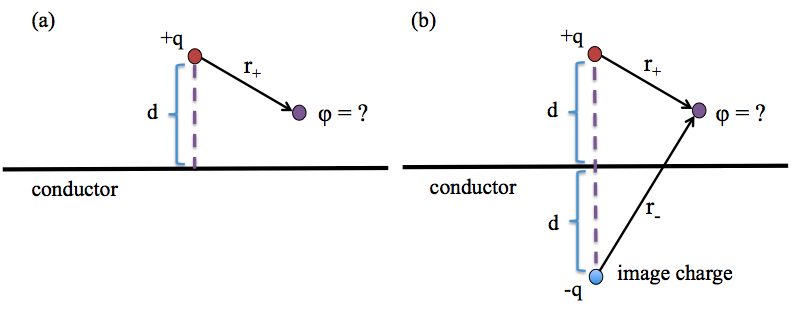
\includegraphics[width=5.5in]{moi_geo1.png}
\caption{(a) Single point source (charge) above an infinitely long conducting surface. (b) The same geometry, but with a virtual source point (with opposite charge) located symmetrically across the conducting plane.}
\label{MOI_geo1}
\end{figure}

We consider a single point source (charge) in the upper half plane, where it is placed above an infinitely long conducting surface. This is illustrated in Figure(\ref{MOI_geo1}a). We are interested in what the \emph{electric field}, or just vector field, $\phi$, looks like at another point in the plane. The governing problem is that of \emph{Poisson} problem, an elliptic PDE, 
$$\Delta \phi = -\frac{q}{\epsilon_0} \delta({\bf{r}} - {\bf{r}}_0),$$ where ${\bf{r}}_0 = d \hat{z},$ the location of the point source, $+q$, and $\phi$ is the potential associated with such point source. We note that for any non-homogeneous differential equation, we will have both a complementary solution and particular solution. Our only boundary condition is that on the conducting surface, say at $z=0$, the potential is zero. \\

This is where the intuition behind the method of images is beautiful. Rather than look for a particular solution, say $\phi_+$, and a complementary solution, $\phi_{-}$, to the equations $$\Delta \phi_+ = -\frac{q}{\epsilon_0} \delta({\bf{r}}-{\bf{r}}_0) \  \ \  \mbox{ and } \ \ \ \Delta \phi_{-}= 0,$$ respectively, we will try to cook up a solution that satisfies the boundary condition at $z=0$ using knowledge of the fundamental solution of such elliptic operator, e.g., $\Delta$ in $2D$.\\

We note that the general potential for such an operator is given by $\phi = \frac{k}{r}$, where $k$ is a constant that is determined by the physics in the underlying problem. Here $k=\frac{\pm q}{4\pi\epsilon_0},$ where $\pm q$ depends on which source term you are considering. If we need combine these two solutions, we note we can satisfy the boundary condition at $z=0$, if we place a point charge of equal and opposite sign at the mirror image of the other charge below the plane. This is seen in Figure(\ref{MOI_geo1}b).\\

\emph{Note} that below the plane is not even in the original domain of the problem, hence when we consider the Poisson-type problem for it's source charge, we find $$\Delta \phi_{-} = \delta( {\bf{r}}-{\bf{r}}_{im}) = 0,$$ where ${\bf{r}}_{im} = -d \hat{z},$ since ${\bf{r}}_{im}$ is not in the domain of the problem at hand.\\

Therefore the solution to this Poisson problem is $$\phi = \phi_{+} + \phi_{-} = \frac{1}{4\pi\epsilon_0} \left[  \frac{q}{r_+} + \frac{-q}{r_{-}}  \right] =\frac{1}{4\pi\epsilon_0} \left[ \frac{q}{\sqrt{x^2 + (z-d)^2 }} + \frac{-q}{\sqrt{x^2 + (z+d)^2}}  \right] $$


%
% Subsection: Example: Point Charge and Grounded Sphere
%
\subsection{Example: Point Charge and a Grounded Sphere}

\begin{figure}[h!]
\centering
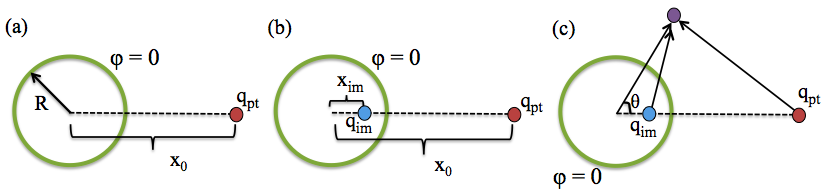
\includegraphics[width=6.25in]{moi_geo2.png}
\caption{(a) Single point source of charge $q_{pt}$ outside a grounded sphere. (b) The same geometry, but with a virtual source point (with differing) located inside the grounded sphere at an unknown location, $x_{im}$. (c) Illustrating the influence from both the point charge and image point charge on a point outside the sphere.}
\label{MOI_geo2}
\end{figure}

Consider the problem of a point charge outside of a grounded sphere.  Since the sphere is grounded, we need the potential to be equal to zero on the entire sphere. This is our boundary condition. To setup the geometry, say the point charge is a distance $x_0$ away from the sphere of radius, $R$.  For simplicity, we will also center the sphere about the origin. This is shown below in Figure(\ref{MOI_geo2})(a). \\ 

In order to find the potential everywhere using the method of images, we must need to find the location of the virtual point charge, such that the boundary condition on the sphere is satisfied. To do this, we make the hypothesis, that to preserve symmetry, this image point should be placed somewhere along the $x-axis$, and moreover, to satisfy that $\phi = 0$ along the sphere, intuition suggests this point will need to be inside the sphere.\\

Rather than try to calculate the potentials of both these points to satisfy the boundary condition along the entire sphere, we consider trying to satisfy the boundary condition at two points along the $x$-axis, namely $(R,0)$ and $(-R,0)$, i.e.,

\begin{itemize}
\item At $(R,0)$, $\phi = 0$
\item At $(-R,0)$, $\phi=0.$
\end{itemize}

If this doesn't make sense why we only consider these two points, we have somewhat pulled a fast one. Well, not really. We are just using what scientists call \emph{hindsight}, err I mean, foresight when thinking about a problem. The motivation is as follows. We note that using the fundamental solution for $\Delta\phi=0$ in radial coordinates in $2-D$ for electrostatics problems, we will have two unknowns when placing the image point - the location along the $x$-axis and the strength of the charge. The train of thought then follows that by using as much symmetry as possible, if we are able to write a system of two equations and two unknowns, we then can get all the information we need for finding the true solution. 

Therefore from those two (more specific) boundary conditions, we get
\begin{align*}
\phi \Big|_{(x,y)=(R,0)} = 0 &=\frac{1}{4\pi\epsilon_0} \left[ \frac{q_{pt}}{(x_0 - R)} +  \frac{q_{im}}{(R-x_{im})} \right] \\
\phi\Big |_{(x,y)=(-R,0)} = 0  &= \frac{1}{4\pi\epsilon_0}\left[ \frac{q_{pt}}{(x_0 + R)}  +  \frac{q_{im}}{(x_{im}+R)} \right].
\end{align*}

Solving the above system of two equations and two unknowns yields, 
$$x_{im} = \frac{R^2}{x_0} \ \ \ \mbox{ and } \ \ \ q_{im} = \frac{-q_{pt} R}{x_0}.$$

Now to calculate the potential of any point outside the sphere, $(r,\theta,\phi)$, we find 
$$\phi(r,\theta,\phi) = \phi_{pt}\Big |_{(r,\theta,\phi)} + \phi_{im}\Big|_{(r,\theta,\phi)} = \frac{1}{4\pi\epsilon_0} \left[ \frac{q_{pt}}{\sqrt{r^2+x_0^2- 2rx_0\cos\theta}} + \frac{-\frac{q_{pt}R}{x_0}}{\sqrt{r^2+\frac{R^4}{x_0^2} - 2r\frac{R^2}{x_0}\cos\theta}}  \right].$$

At this junction, you may be wondering whether or not the above solution truly satisfies the boundary condition on the entire sphere. Well, the nice thing about PDEs (and differential equations in general) is we can always check out solution. (\emph{If time permits on tests, of course...})\\

We first consider an arbitrary point on the sphere, say distances from charges $q_{pt}$ and $q_{im}$ of
$$d_{pt} = \sqrt{R^2+x_0^2 -2Rx_0\cos\theta} \ \ \ \mbox{and} \ \ \ d_{im} = \sqrt{R^2+\left(\frac{R^2}{x_0}\right) - 2R\left(\frac{R^2}{x_0}\right)\cos\theta},$$

respectively. Now the potential on the surface of the sphere is given by
\begin{align*}
\phi \Big|_{r=R} &= \frac{1}{4\pi\epsilon_0}\left[ \frac{q_{pt}}{d_{pt}} + \frac{q_{im}}{d_{im}}  \right]  \\
&= \frac{1}{4\pi\epsilon_0} \left[ \frac{q_{pt}}{\sqrt{R^2+x_0^2- 2Rx_0\cos\theta}} + \frac{-\frac{q_{pt}R}{x_0}}{\sqrt{R^2+\frac{R^4}{x_0^2} - 2R\frac{R^2}{x_0}\cos\theta}}  \right] \\
&= \frac{1}{4\pi\epsilon_0} \left[ \frac{q_{pt}}{\sqrt{R^2+x_0^2- 2Rx_0\cos\theta}} + \frac{q_{pt}}{\sqrt{ \frac{x_0^2}{R^2}\left( R^2+\frac{R^4}{x_0^2} - 2\frac{R^3}{x_0}\cos\theta  \right)           } }  \right] \\
&= \frac{1}{4\pi\epsilon_0} \left[ \frac{q_{pt}}{\sqrt{R^2+x_0^2- 2Rx_0\cos\theta}} - \frac{q_{pt}}{\sqrt{x_0^2+R^2 -2Rx_0\cos\theta}} \right] \\
&= 0.
\end{align*}

Hence our solution checks out!

\newpage
\graphicspath{{./Physics/}}

\section{Physics!}

\emph{You're taking physics? I love physics!}, said only $5\%$ of the population, of which $90\%$ were being ironic. It's no surprise that physics gets a bad rap somewhere between birth and college graduation; however, it is truly a beautiful science and arguably without it, modern mathematics would not be where it is today with it. For much of mathematics conception, math and physics (and other sciences for that matter) were like peas and carrots. It has only been within the last century or so, where people starting differentiating between calling themselves scientists to mathematicians, physicists, chemists, or biologists. I digress. Physics has a place, and from it come a lot of interesting and useful mathematics!\\

In this section we will give a crash course in basic physics ideas, e.g., conservation laws and basic mechanics, which will then lead us down the rabbit hole of \emph{calculus of variations} to learn Lagrangian and Hamiltonian formulations of mechanics. I apologize in advance for attempting to sum up years worth of courses in a minimal amount of words. There will be (many) things left out, so please do some light (gravity pun?) reading for further insight and intuition. Buckle up, we're about to see math in action!\\


%%%%%%%%%%%%%%%%%%%%%%%%%%%%%%%%%%
%
% SECTION: BASIC PHYSICS PRINCIPLES
%
%%%%%%%%%%%%%%%%%%%%%%%%%%%%%%%%%%

\subsection{Basic Physics Principles}

There once lived a man named Isaac Newton. He may have invented calculus (or co-discovered at the same time as his rival Gottfried Leibniz). What led him to calculus was his fascination with phenomena in the natural world and wanting to quantify the beauty he saw through formulae and equations. Upon doing so, he eventual wrote \emph{Philosophiae Naturalis Principia Mathematica}, which was to be a large collection of how the universe operated. Whilst his law of gravitation did not hold up past two centuries, although it is a very good approximation in the non-relativistic regime, his laws of motion remain infamous, especially with students being introduced to physics for the very first time. \\

Newton's three laws of motion are as follows
\begin{enumerate}
\item  An object stays at rest (or continues to move at constant velocity) unless an external force acts upon it.
\item The sum of all external forces acting on an object is equal to the product of the object's mass and acceleration.
\item When a body exerts a force on a second body, the second body simultaneously exerts an equal in magnitude, but opposite in direction, force on the first body.
\end{enumerate}

We will now give a more mathematical flavor of the three laws of motion.\\

\begin{itemize}

%
% LAW 1
%
\item[] {\bf{Law 1}}: \\ \\

The first law basically states if the sum of all forces on an object are zero, then the object is either at rest or moving at a constant velocity, e.g., it is not accelerating. More specifically it says that the \emph{vector} sum of all forces is zero. This law is better known as the \emph{law of intertia}. \\ 

Mathematically it says the following two statements are equivalent,
$$\sum_{j=0}^N {\bf{F}}_j = 0  \Leftrightarrow \frac{d {\bf{v}}}{dt} = 0,$$

where ${\bf{F}}_j$ is a force acting on a body and ${\bf{v}}$ is the velocity of such body. These statements say that if the body is in motion, it will remain in motion, moving in a straight line, until other forces act upon it. Furthermore, this is evident in what is referred to as the \emph{Newtonian reference frame}, or \emph{intertial} reference frame, where the motion of a body according to another observer remains moving at constant speed in a straight line. \\

%
% LAW 2
%
\item[] {\bf{Law 2}}: \\ \\

Newton's second law of motion is really a statement about the \emph{conservation of momentum}. In a nutshell it states that the time rate of change of linear momentum is equal to the sum of  forces acting on the body in an inertial reference frame. This can be described mathematically as

$$\frac{d{\bf{p}}}{dt} = \frac{ d(m{\bf{v}})}{dt} = \sum_{j=0}^N {\bf{F}}_j,$$

where ${\bf{p}}$ is the linear momentum, and is equal to mass times velocity, i.e., ${\bf{p}} = m{\bf{v}}.$ We note that this is consistent with the first law, in that if the sum of vector forces acting on a body is zero, then the momentum of the object remains unchanged. A consequence of any net force is a change in momentum of a body. \\

It is common to assume that the mass of a body does not change and is constant, leading to the infamous $$F_{net} = \sum_{j=0}^N {\bf{F}}_j = m \frac{d{\bf{v}}}{dt} = m \frac{d^2 {\bf{x}}}{dt^2} = m{\bf{a}};$$

however if mass does change, we need to consider $$F_{net}  + {\bf{u}} \frac{dm}{dt}  = \frac{d{\bf{v}}}{dt},$$ where ${\bf{u}}$ is the velocity of the escaping (or incoming) mass of the body. The extra term, ${\bf{u}} \frac{dm}{dt}$ is sometimes referred to as the advection of momentum. We note that if the body's mass is changing we do not simply treat the original statement as a product rule, i.e., $$\mbox{WRONG} \Rightarrow \ \ {\bf{F}}_{net} = \frac{d}{dt}(m{\bf{v}}) = m\frac{d{\bf{v}}}{dt} + {\bf{v}}\frac{dm}{dt} \ \ \ \Leftarrow \mbox{WRONG}.$$

The reason for this is that it does not respect Galilean invariance, or that the laws of motion must remain the same regardless of what inertial system you are in, e.g., our statement above would violate that in one frame of reference ${\bf{F}}=0$ while in another ${\bf{F}}\neq 0$. For example, say in one reference frame you are moving at constant velocity $U$, while we consider another non-moving (stationary) reference frame. We can relate the physics between the two using Galilean transformations, i.e., 
\begin{align*}
x' &= x - Ut \ \ \ \ \mbox{(position)} \\
v' &= \frac{dx'}{dt} = \frac{dx}{dt} - U \\
a' &= \frac{d^2 x'}{dt^2} = \frac{d^2 x}{dt^2} = a, \\
\end{align*} 

where all coordinates with primes indicate the moving inertial reference frame. Hence in both frames of reference we have the same acceleration, and hence conservation of momentum is preserved. \\

Moreover, if we wish to consider Newton's second law of motion for relativistic systems, we need to change our definition of linear momentum, since at speeds ``near-ish" to the speed of light, linear momentum is not simply the product of mass and velocity. \\

Newton's second law of motion is very powerful, and is the law that most people refer to the most when considering physical phenomena. For example, the main equations of fluid dynamics, called the \emph{Navier-Stokes} equations, although nonlinear PDEs, are just a statement about the conservation of momentum for a fluid. At the heart of basic mechanics, Newton's second law is main driver to solutions. 

%
% LAW 3
%
\item[] {\bf{Law 3}}: \\ \\

The crux of Newton's third law is that no force is only unidirectional. If body A exerts a force on body B, body B exerts the same force back on body A. All forces must be interactions between bodies, and no one body can magically exert a force without feeling the equal and opposite force back upon itself. \\

Think about punching a wall. You may think you have exerted all the force onto the wall, but the reason your hand hurts is because the wall has ``hit your hand" back with as much force as you placed against it. To every action, there is an equal and opposite reaction. 

\end{itemize}

We will now briefly discuss some conversation laws, or integrals of the system, in physics.



%%%%%%%%%%%%%%%%%%%%%%%%%%%%%%%%%
%
% Conservation Laws
% 
%%%%%%%%%%%%%%%%%%%%%%%%%%%%%%%%%

\subsubsection{Conservation Laws}

If a system is closed, e.g., \emph{isolated}, and the system does not interact with its background environment in any way, certain quantities arise, which are preserved throughout the entire evolution of the system considered. These quantities are known as integrals of the system, constraints of the motion, or conserved quantities. In physics, we call them conservation laws, and there are three:

\begin{enumerate}
\item Conservation of Momentum 
\item Conservation of Energy
\item Conservation of Angular Momentum
\item Conservation of Charge
\end{enumerate}

We will now briefly describe each of these conservation laws. Well not, conservation of charge, but that should be somewhat self explanatory for the level of physics we are shooting for. Note, in mathematics the term conservation law usually refers to transport type hyperbolic equations of the form, here in their scalar-ized glory, $$\partial_t u + \partial_x f(u) = 0.$$

$u$ is called the conserved quantity, while $f$ is called the flux.  

\begin{itemize}

%
%  Conservation of Momentum
% 
\item[] {\bf{Conservation of Momentum}} \\ \\

We have already seen a bit about the conservation of momentum coming from Newton's second law of motion. Rather than think about forces causing changes in momentum of a body, let's consider the momentum in a system as a whole. If one part of the system gains momentum to go one way in the system, another part of the system must have gained equal momentum, but to go in the opposite direction. \\

If we consider our system to have two particles in it, we assume that at time, $t_1$, and later time $t_2$, the total momentum of the system must be the same, e.g.,

$$\Big[ m_1 {\bf{v}}_1 + m_2 {\bf{v}}_2\Big]\ \Bigg|_{t=t_1} = \Big[ m_1 {\bf{v}}_1 + m_2 {\bf{v}}_2\Big] \ \Bigg|_{t=t_2}.$$ 

However, the above assumes that if there have been any collisions between the balls, that only \emph{elastic} collisions have occurred. That is to say, no energy has been lost, well converted, to heat, sound, etc. Spoiler alert - energy cannot be created nor destroyed, merely converted to other forms of energy. Those type of collisions where energy has been converted to heat (sound, etc.) are called \emph{inelastic} collisions. We will discuss this further in the conservation of energy section. 

Again, the main statement about the conservation of momentum is best summed up (heyyo!) through Newton's second law,
$$m \frac{d{\bf{v}}}{dt} = \sum_{j} {\bf{F}}_j.$$

Let's do some mechanics problems to illustrate the power of this law! In doing so, we will also try to motivate intuitive ideas on how to approach such mechanics problems.








\end{itemize}
\newpage
\graphicspath{{./Asymptotics/}}


%
%
%
%
\section{Asymptotics and Perturbation Methods}

This section will have a vastly different flavor, in comparison to the previous methods. We are to be no longer concerned with exact solutions to equations, even in the form of an infinite sum, but will set our sights solely on asymptotic or perturbative solutions. You can think of these as \emph{very} good approximation methods, if you've never heard the lingo prior. Well, let's just define these when the time comes, but now be comforted by knowing we will solely search for ``approximate" solutions to equations now. 


%
%
% INTEGRAL ASYMPTOTICS AND LAPLACE'S METHOD
%
%
\subsection{Integral Asymptotics and Laplace's Method}

First we consider the seemingly innocent integral, $I(\lambda)$,
\begin{equation}
\label{laplace_integral} I(\lambda) = \int_a^b f(t) e^{-\lambda g(t) } dt.
\end{equation}

Now what I haven't revealed was properties about $f(t)$, $g(t)$, or $\lambda$. Well, we'll assume $f$ and $g$ are friendly functions, where friendly for us just means that they are smooth enough to be replaced by local Taylor series approximations of appropriately desired degree. 

Well, what about $\lambda$? This where the term \emph{asymptotic} comes into play. We are only concerning ourself here with the behavior of $I(\lambda)$ as $\lambda\rightarrow\infty$. Hence are only on a mission to look at this integral in a limiting behavior scenario. This is the general idea with asymptotic methods, that is, methods that describe limiting behavior of a function, or solution to an equation. We will now briefly give two definitions to solidify this idea.  

\begin{definition}
We say to functions $f_1$ and $f_2$ of a natural number parameter $n$, are \textbf{asymptotically equivalent}, e.g., $f_1(n) \sim f_2(n)$ (as $n\rightarrow\infty$), if and only if $\lim_{n\rightarrow\infty} \frac{f(n)}{g(n)}=1$. This equivalence only holds in the sense of the limit, though.
\end{definition}

For example, consider the functions $g(n) = n^2 - 2n$ and $h(n) = n^2 + 3n + 7$. It clear that that $g(n)\neq h(n) \forall n\in\mathbb{N}$; however, it is clear that $g(n)\sim h(n)$ as $n\rightarrow\infty$, so it is safe to say that $g(n)$ and $h(n)$ are asymptotically equivalent as $n\rightarrow\infty.$ It is paramount to note that we had to state the asymptotic equivalent only holds ``as $n\rightarrow\infty$". In general, the limiting behavior does not have to be as $n\rightarrow\infty$ or even $n\rightarrow0$, it just needs to be at a point of interest for the functions, e.g., where a function may become singular, etc.  Using this idea, we will now explore what an asymptotic expansion of a function is. 

\begin{definition}
An \textbf{asymptotic expansion} of a function $f(x)$ is an expression of $f(x)$ in terms of a series, such that by taking any initial partial sum provides an asymptotic formula for $f(x)$. The successive terms in the series provide an increasing accurate description of $f(x)$, by giving more detail to the growth of $f(x)$. We note that the partial sums of this expansion do not necessarily converge. 
\end{definition} 

Now let's get back to the problem at hand, finding the limiting behavior of (\ref{laplace_integral}) as $\lambda\rightarrow\infty$. To achieve this, we will use \emph{Laplace's Method}.

%
% LAPLACE'S METHOD w/ minimum on interior of integration bounds
%
\subsubsection{Laplace's Method}

Consider (\ref{laplace_integral}), such that $g(t)$ assumes a strict minimum in $[a,b]$ at an interior point, call it $c$. We will also assume that $g'(c)=0$ (duh), $g''(c)>0$ (so the point is a minimum, duh), and $f(c)\neq 0$. Using the secret mathematician trick of adding and subtracting zero, we can rewrite (\ref{laplace_integral}) as

$$I(\lambda) = e^{-\lambda g(c)} \int_a^b f(t) e^{ -\lambda\big[ g(t) - g(c) \big] } dt.$$

This is the part that is crucial for Laplace's Method. Since $g(c)$ is a minimum of $g(t)$ on $[a,b]$, for $\lambda>>1$, the main contribution of $I(\lambda)$ will come from a small neighborhood of $c$. This is more obvious from the definition of $I(\lambda)$ above, rather than where it was first introduced. Hence for $\lambda>>1$, 

\begin{align*}
I(\lambda) &\approx e^{-\lambda g(c)} \int_{c-\epsilon}^{c+\epsilon} f(t) e^{ -\lambda\big[ g(t) - g(c) \big] } dt \\ \\
	& \approx  e^{-\lambda g(c)} f(c) \int_{c-\epsilon}^{c+\epsilon} e^{ -\lambda\big[ g(t) - g(c) \big] } dt  \\ 
\end{align*}

Next we approximate $g(t)$ by its Taylor series centered around $t=c$, 
$$g(t) = g(c) +(t-c)g'(c) + \frac{1}{2!} (t-c)^2 g''(c) + \mathcal{O}( (t-c)^3 ).$$

Substituting the above into the integral equation, we find

\begin{align*}
I(\lambda) &\approx e^{-\lambda g(c)} f(c) \int_{c-\epsilon}^{c+\epsilon} e^{ -\lambda\big[ \big( g(c) +(t-c)g'(c) + \frac{1}{2!} (t-c)^2 g''(c) \big) - g(c) \big] } dt \\ \\
	& \approx  e^{-\lambda g(c)} f(c) \int_{c-\epsilon}^{c+\epsilon} e^{ -\lambda\big[  g'(c)(t-c) + \frac{1}{2!}  g''(c)(t-c)^2 \big] } dt  \\  \\
	&= e^{-\lambda g(c)} f(c) \int_{c-\epsilon}^{c+\epsilon} e^{ - \frac{\lambda}{2}  g''(c)(t-c)^2 } dt  \\  
\end{align*}

since $g'(c)=0$. Recall we said the main contribution of $I(\lambda)$ comes from a neighborhood of $c$. Moreover, on the flip side, we assume the integral's contribution outside that neighborhood, therefore we can expand that neighborhood to all of $\mathbb{R}$, i.e., we now have

\begin{equation*}
I(\lambda)  \approx e^{-\lambda g(c)} f(c) \int_{-\infty}^{\infty} e^{ - \frac{\lambda}{2}  g''(c)(t-c)^2 } dt.
\end{equation*}

Next to integrate the Gaussian-type integral above, we first do the swanky transformation of letting $s = t-c$, and getting

\begin{align*}
I(\lambda) &\approx e^{-\lambda g(c)} f(c) \int_{-\infty}^{\infty} e^{ - \frac{\lambda}{2}  g''(c)s^2 } ds  \\ \\
	&= e^{-\lambda g(c) } f(c) \sqrt{ \frac{2\pi}{\lambda g''(c) } }.
\end{align*}

Thus to leading order we have that 

\begin{equation}
\label{std_laplace} I(\lambda) \sim  e^{-\lambda g(c) } f(c) \sqrt{ \frac{2\pi}{\lambda g''(c) } } \ \ \ \mbox{ as } \lambda\rightarrow\infty.
\end{equation}

This above is the standard Laplace Method's result when the minimum is within the interval $(a,b)$. There are three basic ideas behind this methodology. They are as follows:
\begin{enumerate}
\item Since we are concerned with $\lambda\rightarrow\infty$, the main contribution of $I(\lambda)$ comes from a small neighborhood of the point in which $g(t)$ is at its local minimum, say $t=c$, and can replace the integration bounds from $[a,b] \rightarrow [c-\epsilon, c+\epsilon]$.
\item Within the neighborhood of the minimizer, we can approximate $f(t)$ and $g(t)$ with their Taylor Series until desired order. 
\item Since the main contribution of $I(\lambda)$ is coming from the interval $ [c-\epsilon, c+\epsilon]$, we can extend this interval to $[-\infty,\infty]$, as the regions outside $ [c-\epsilon, c+\epsilon]$ only contribute higher order terms to $I(\lambda)$ as $\lambda\rightarrow\infty$.
\end{enumerate}

We will now go through a very similar calculation to illustrate what happens when the minimum of $g(t)$ in on an end point of the integration bounds, but first we will show the trick for integrating Gaussian-type integrals.


%
% GAUSSIAN INTEGRAL 
%
\subsubsection{Gaussian Integral}

We will show how to explicitly integrate integrals of the form, 
\begin{equation}
\label{gauss_integral} G = \int_{-\infty}^{\infty} e^{-x^2} dx.
\end{equation}

To do this, we will transform this integral to polar coordinates, but first, we will do the magical trick. This is it. Just square (\ref{gauss_integral}), i.e.,

$$G^2 = \int_{-\infty}^{\infty} e^{-x^2} dx  \int_{-\infty}^{\infty} e^{-y^2} dy=  \int_{-\infty}^{\infty}  \int_{-\infty}^{\infty} e^{-(x^2+y^2)} dxdy.$$ 

Now since $G^2$ is in $2D$, we can transform it to polar coordinates, by letting $r^2 = x^2+y^2$ and $rdrd\theta = dxdy$. We have

$$G^2 =  \int_{0}^{\infty}  \int_{0}^{2\pi} e^{-r^2} rdrd\theta.$$

Therefore on the above we can simply do the substitution $let u = r^2$ and therefore $du = 2rdr$. We now have

$$G^2 =   \int_{0}^{\infty}  \int_{0}^{2\pi} \frac{1}{2} e^{-u} dud\theta,$$

and hence

$$G^2 = - \pi e^{-u} \bigg|_{0}^{\infty} = \pi.$$

Now solving for $G$, we get that 

$$G = \sqrt{pi}.$$

We used this trick above to find the leading order behavior of the Laplace Integral, and will use it again in a minute for a similar computation! 


%
% LAPLACE'S METHOD w/ minimum on edge of integration bounds 
%
\subsubsection{Laplace's Method Take Two (minimizer on an integration bound)}

Consider (\ref{laplace_integral}), such that $g(t)$ assumes a strict minimum in $[a,b]$ at an endpoint of the interval. Without loss of generality, let's just say the minimum is found at $t=a$. We will also assume that $g'(a)=0$ (duh), $g''(a)>0$ (so the point is a minimum, duh), and $f(a)\neq 0$. Using the same math trick of adding and subtracting zero, we can rewrite (\ref{laplace_integral}) as

$$I(\lambda) = e^{-\lambda g(a)} \int_a^b f(t) e^{ -\lambda\big[ g(t) - g(a) \big] } dt.$$

We will make the same assumptions as we did above, e.g., that the main contribution to $I(\lambda)$ comes from a neighborhood of $t=a$, $f(t)$ and $g(t)$ are smooth enough so that we can replace them by their Taylor Series centered at $t=a$, and that since the main contribution is coming a neighborhood of $t=a$, we will be able to expand this neighborhood to all of $\mathbb{R}^+$ with only higher order asymptotic terms being affected. The reason for only blowing this interval up to $[a,\infty)$ is because we do not consider points $t<a$. Upon doing these things, we get

\begin{align*}
I(\lambda) &\approx e^{-\lambda g(a)} \int_{a}^{a+\epsilon} f(t) e^{ -\lambda\big[ g(t) - g(a) \big] } dt \\ \\
	& \approx  e^{-\lambda g(a)} f(a) \int_{a}^{a+\epsilon} e^{ -\lambda\big[ g(t) - g(a) \big] } dt  \\  \\
	&\approx e^{-\lambda g(a)} f(a) \int_{a}^{c+\epsilon}  e^{ -\lambda\big[ \big( g(a) +(t-a)g'(a) + \frac{1}{2!} (t-a)^2 g''(a) \big) - g(a) \big] } dt \\ \\
	& \approx  e^{-\lambda g(a)} f(a) \int_{a}^{c+\epsilon} e^{ -\lambda\big[  g'(a)(t-a) + \frac{1}{2!}  g''(a)(t-a)^2 \big] } dt  \\  \\
	&= e^{-\lambda g(a)} f(a) \int_{a}^{a+\epsilon} e^{ - \frac{\lambda}{2}  g''(a)(t-a)^2 } dt  \\  \\
	&  \approx e^{-\lambda g(a)} f(a) \int_{a}^{\infty} e^{ - \frac{\lambda}{2}  g''(a)(t-a)^2 } dt.
\end{align*}

Now doing the same substitution as before, letting $s=t-a$, we are left with the following Gaussian-type integral to integrate,

\begin{align*}
I(\lambda) &\approx e^{-\lambda g(a)} f(a) \int_{0}^{\infty} e^{ - \frac{\lambda}{2}  g''(a)s^2 } ds  \\ \\
	&= e^{-\lambda g(a) } f(a) \sqrt{ \frac{\pi}{2\lambda g''(a) } }.
\end{align*}

Thus when the minimizer is at an endpoint, we have to leading order that 

\begin{equation}
\label{endpoint_laplace} I(\lambda) \sim  e^{-\lambda g(a) } f(a) \sqrt{ \frac{\pi}{2\lambda g''(a) } } \ \ \ \mbox{ as } \lambda\rightarrow\infty.
\end{equation}


%
% THE GAMMA FUNCTION AND HIGHER ORDER ASYMPTOTICS
%
\subsubsection{The Gamma Function and Higher Order Asymptotics}

Usually in the asymptotic business, the next thing one is introduced to is the \emph{Gamma function}. The reason for this is two-fold; first it is a generalization of the factorial function, and second, it is used to derive Stirling's approximation, which is looking at the asymptotic behavior of the factorial function itself. We will do all these things, but before, we concern ourself with the asymptotic behavior of the factorial, let's use the Gamma function to look at higher order asymptotics associated with the Laplace integral. 

The Gamma function is defined as, 
\begin{equation}
\label{gamma_function} \Gamma(x) = \int_0^\infty t^{x-1} e^{-t} dt.
\end{equation}

The way to see (\ref{gamma_function}) is a continuous generalization of the factorial function, we simply have to integrate it by parts, e.g., 
\begin{align*}
\Gamma(x+1) &= \int_0^\infty t^x e^{-t} dt \\ \\
	&= - t^{x} e^{-t} \bigg|_{0}^\infty + \int_{0}^{\infty} x t^{x-1} e^{-t} dt \\ \\
	&= x \int_{0}^{\infty} t^{x-1} e^{-t} dt \\ \\
	&= x\Gamma(x).
\end{align*}

Thus if $x=n\in\mathbb{Z}^+$, we have $$\Gamma{(n+1)}=n!.$$

Now we can use this to find higher-order asymptotic terms in vein of the Laplace integral in (\ref{laplace_integral}). We will again assume  that $g(t)$ assumes a strict minimum over $[a,b]$ at a point $c\in(a,b)$, as well that $g'(c)=0, g''(c)\neq0,$ and $f''(c)\neq 0.$ Now where this calculation is different than those previously done is that we assume $f(c)=0$. This subtle change will lead us to employ the Gamma function to find the leading behavior in our asymptotic expansion. We will again make the same assumptions as before, e.g., the main contribution comes from the neighborhood of $t=c$, and all that jazz. Now for $\lambda>>1$,

\begin{align*}
I(\lambda) &=  \int_a^b f(t) e^{-\lambda g(t) } dt \\ \\
	&\approx e^{-\lambda g(c)} \int_{c-\epsilon}^{c+\epsilon} f(t) e^{-\lambda \big( g(t) - g(c) \big) } dt \\ \\
	&= e^{-\lambda g(c)} \int_{c-\epsilon}^{c+\epsilon}  \left[ f(c) + f'(c)(t-c) + \frac{1}{2!} f''(c) (t-c)^2 + \mathcal{O}( (t-c)^3 )  \right] e^{- \lambda \big( g'(c)(t-c) + \frac{1}{2!} g''(c)(t-c)^2 +  \mathcal{O}( (t-c)^3 ) \big) } dt \\ \\
	&\approx e^{-\lambda g(c)} \int_{c-\epsilon}^{c+\epsilon}  \left[  f'(c)(t-c) + \frac{1}{2!} f''(c) (t-c)^2 \right] e^{- \frac{\lambda}{2}  g''(c)(t-c)^2 } dt \\ \\
	&= \frac{f''(c)}{2} e^{-\lambda g(c) }  \int_{c-\epsilon}^{c+\epsilon} (t-c)^2 e^{-\frac{\lambda}{2} g''(c) (t-c)^2 } dt.\\
\end{align*}

We do the same transformation $s = t-c$, and then expanding the integration region to all of $\mathbb{R}$, we obtain
\begin{align*}
I(\lambda) &\approx  \frac{f''(c)}{2} e^{-\lambda g(c) }  \int_{-\infty}^{\infty} s^2 e^{-\frac{\lambda}{2} g''(c) s^2 } ds\\ \\
	&= f''(c) e^{-\lambda g(c) } \int_0^{\infty} s^2 e^{-\frac{\lambda}{2} g''(c) s^2 } ds. \\ 
\end{align*}

To simplify the above integral, we perform one more transformation. Letting $u = \frac{\lambda}{2}g''(c) s^2$ and hence $du = \lambda g''(c) s ds$, we find that
\begin{align*}
I(\lambda) &\approx f''(c) e^{-\lambda g(c) } \int_0^{\infty} \left( \frac{2u}{\lambda g''(c) } \right) e^{-u} \left( \frac{du}{2\lambda g''(c) u} \right) \\ \\
	&= f''(c) e^{-\lambda g(c) } \int_{0}^{\infty} \frac{ \sqrt{2} }{ (\lambda g''(c) )^{3/2} } u^{1/2} e^{-u} du \\ \\
	&= \frac{ \sqrt{2} f''(c) }{ (\lambda g''(c) )^{3/2} } e^{-\lambda g(c) } \Gamma\left(\frac{3}{2}\right) \\ \\
	&= \frac{ \sqrt{2} f''(c) }{ (\lambda g''(c) )^{3/2} } e^{-\lambda g(c) } \left( \frac{1}{2} \right) \Gamma\left( \frac{1}{2} \right) \\ 
 \end{align*}
 
 Now we find that $$\Gamma\left( \frac{1}{2} \right) = \sqrt{ \pi }, i.e.,$$
\begin{align*}
\Gamma\left( \frac{1}{2} \right) &= \int_0^{\infty} t^{-1/2} e^{-t} dt, \ \ \ \ \mbox{ let } u=t^{1/2} \\ \\
	&= 2 \int_0^{\infty} e^{-u^2}  du \\ \\
	&= \sqrt{\pi}. \\
\end{align*} 
 
 Hence we find that 
 $$I(\lambda) \approx \sqrt{ \frac{\pi}{2} } \frac{ f''(c) }{ ( \lambda g''(c) )^{3/2} } e^{-\lambda g(c) }.$$
 
 Therefore we have to leading order,
 
 $$I(\lambda) \sim f''(c) e^{-\lambda g(c) } \sqrt{  \frac{\pi}{ 2 \left( \lambda g''(c) \right)^3   } }, \ \ \ \ \mbox{ as } \lambda\rightarrow\infty.$$
 
 
 %
% STIRLING'S APPROXIMATION
%
\subsubsection{Striling's Approximation}
 
 We now set our sights on deciphering the leading order asymptotics of $n!$ as $n\rightarrow\infty$. To do this we will rightfully use Laplace's method, but first will motion to massaging the Gamma function into a more welcoming form for Laplace's method. Consider
 
$$\Gamma\left( x+1 \right) = \int_0^\infty t^x e^{-t} dt.$$

I hope you remember your exponential and logarithmic identities. We are about to go for a walk down memory lane. First let's warmup and use the property that $$t^x = e^{ x\ln(t) }$$,

$$\Gamma\left( x+1 \right) = \int_0^\infty e^{ x\ln(t) } e^{-t} dt = \int_0^{\infty} e^{-x \left( \frac{t}{x} - \ln(t)  \right) } dt.$$

Next we perform a substitution, $z = \frac{t}{x}$ (and $dz = \frac{1}{x} dt$), and get

$$\Gamma\left( x+1 \right) = x \int_0^\infty e^{-x \left(  z-\ln(xz) \right) } dz = x \int_0^\infty e^{-x \left(  z-\ln(x)-\ln(z) \right) } dz = xe^{x\ln(x)} \int_0^\infty e^{-x\left(  z-\ln(z)  \right) } dt.$$

We now have exponentially and logarithmically massaged the Gamma integral into the following form,

\begin{equation}
\label{stirling_gamma_int} \Gamma\left( x+1 \right) = x^{x+1} \int_0^\infty e^{-x \left( z - \ln z \right) } dz.
\end{equation}

We see that (\ref{stirling_gamma_int}) is in the form of a Laplace type integral, with $f(z)=1$ and $g(z) = z - \ln z$. With a  little further analysis, it is clear that $g(z)$ has a strict minimum on $(0,\infty)$ at $z=1$. We see that $g(z=1)=1, g'(1)=0$, and $g''(1)=1.$ Substituting all of this information into the leading order terms of the Laplace integral, we find that 

$$\int_0^\infty e^{-x\left(  z - \ln z \right) } dz \sim e^{-x g(1) } f(1) \sqrt{ \frac{2\pi}{\lambda g''(1) } }  = \sqrt{ \frac{2\pi}{x} } e^{-x}, \ \ \ \mbox{ as } x\rightarrow\infty.$$

Hence we find that the Gamma function has leading order behavior,

$$\Gamma(x+1) \sim x^{x+1} \sqrt{ \frac{2\pi}{x} } e^{-x} = \sqrt{2\pi} x^{ x+\frac{1}{2} } e^{-x}, \ \ \ \mbox{ as} x\rightarrow\infty.$$

To make this a little closer to home, consider $x=n\in\mathbb{Z}^+$, as $n\rightarrow\infty$, that is,  \emph{make n is very large integer}. We are now ready to see what the factorial function looks like as $n$ gets very, very large. 

$$n! \sim \sqrt{2\pi} n^{n+\frac{1}{2}} e^{-n}, \  \ \ \mbox{ as } n\rightarrow\infty.$$
 

\end{document}